%for a more compact document, add the option openany to avoid
%starting all chapters on odd numbered pages
\documentclass[12pt]{cmuthesis}

% This is a template for a CMU thesis.  It is 18 pages without any content :-)
% The source for this is pulled from a variety of sources and people.
% Here's a partial list of people who may or may have not contributed:
%
%        bnoble   = Brian Noble
%        caruana  = Rich Caruana
%        colohan  = Chris Colohan
%        jab      = Justin Boyan
%        josullvn = Joseph O'Sullivan
%        jrs      = Jonathan Shewchuk
%        kosak    = Corey Kosak
%        mjz      = Matt Zekauskas (mattz@cs)
%        pdinda   = Peter Dinda
%        pfr      = Patrick Riley
%        dkoes = David Koes (me)

% My main contribution is putting everything into a single class files and small
% template since I prefer this to some complicated sprawling directory tree with
% makefiles.

% some useful packages
\usepackage{times}
\usepackage{fullpage}
\usepackage{graphicx}
\usepackage{amsmath}
\usepackage{array}
\usepackage{mathptmx}
\usepackage[numbers,sort]{natbib}
\newcolumntype{C}[1]{>{\centering}m{#1}}
\usepackage[backref,pageanchor=true,plainpages=false, pdfpagelabels, bookmarks,bookmarksnumbered,
%pdfborder=0 0 0,  %removes outlines around hyper links in online display
]{hyperref}
\usepackage{subfigure}

% Approximately 1" margins, more space on binding side
%\usepackage[letterpaper,twoside,vscale=.8,hscale=.75,nomarginpar]{geometry}
%for general printing (not binding)
\usepackage[letterpaper,twoside,vscale=.8,hscale=.75,nomarginpar,hmarginratio=1:1]{geometry}

% Provides a draft mark at the top of the document.
\draftstamp{\today}{DRAFT}

\newcommand{\xac}[1]
{{\fontfamily{cmss}\bfseries \color{purple} %XAC: #1% 
}}
\newcommand{\foo}{\hspace{-2.3pt}$\bullet$ \hspace{5pt}}
%\newcommand{\i}[0]{{\em (i)}}
%\newcommand{\ii}[0]{{\em (ii)}}
%\newcommand{\iii}[0]{{\em (iii)}}

\begin {document}
\frontmatter

%initialize page style, so contents come out right (see bot) -mjz
\pagestyle{empty}

\title{ %%{}\it \huge Thesis Proposal}\\
{\bf Making Fabrication Real}\\
{Fabrication for Real Usage, with Real Objects, by Real People}}
\author{Xiang `Anthony' Chen}
\date{August 2016}
\Year{2016}
\trnumber{}

\committee{
Scott Hudson, Co-Chair \\
Stelian Coros, Co-Chair \\
Jodi Forlizzi \\
Tovi Grossman
}

\support{}
\disclaimer{}

% copyright notice generated automatically from Year and author.
% permission added if \permission{} given.

\keywords{Fabrication, 3D printing, real world, design tools}

\maketitle

\begin{dedication}
% To Pigpig
\end{dedication}

\pagestyle{plain} % for toc, was empty

%% Obviously, it's probably a good idea to break the various sections of your thesis
%% into different files and input them into this file...

\begin{abstract}
The increasingly personal and ubiquitous capabilities of computing---everything from smartphones to virtual reality---are enabling us to build a brave new world in the digital realm. Despite these advances in the virtual world, our ability as end-users to transform the physical world still remains limited.

The emergence of low-cost fabrication technology (most notably 3D printing) has brought us a dawn of making, promising to empower everyday users with the ability to fabricate physical objects of their own design. However, the technology itself is oblivious of the physical world---things are, in most cases, assumed to be printed from scratch in isolation from the real world objects they will be attached to and work with.

To bridge this `gulf of fabrication', my thesis research focuses on developing fabrication techniques with tool integration to enable users to expressively create designs that can be attached to and function with existing real world objects. Specifically, my work explores techniques that leverage the 3D printing process to create attachments directly over, onto and around existing objects; a design tool further enables people to specify and generate adaptations that can be attached to and mechanically transform existing objects in user-customized ways; a mixed-initiative approach allows people to create functionally valid objects from their own design, which addresses real world relationships with other objects; finally, by situating the fabrication environment in the real world, a suite of virtual tools allow users to design, make, assemble, install and test physical objects \textit{in situ} directly within the context of their usage.

Overall my thesis aspires to \textit{make fabrication real}---enabling things to be made by real people, to address real usage and to function with real objects in the world.

\end{abstract}

\begin{acknowledgments}

\end{acknowledgments}



\tableofcontents
\listoffigures
\listoftables

\mainmatter

%% Double space document for easy review:
%\renewcommand{\baselinestretch}{1.66}\normalsize

% The other requirements Catherine has:
%
%  - avoid large margins.  She wants the thesis to use fewer pages,
%    especially if it requires colour printing.
%
%  - The thesis should be formatted for double-sided printing.  This
%    means that all chapters, acknowledgements, table of contents, etc.
%    should start on odd numbered (right facing) pages.
%
%  - You need to use the department standard tech report title page.  I
%    have tried to ensure that the title page here conforms to this
%    standard.
%
%  - Use a nice serif font, such as Times Roman.  Sans serif looks bad.
%
% Other than that, just make it look good...


\chapter{Introduction and Overview}

\section{The Disparity of Creativity}
As computers and the Internet become increasingly ubiquitous, people are now able to create or curate a variety of digital content. Today it only takes a few minutes to build and customize a personal website. Anyone can write a beautifully typeset blog without knowing anything about layout, font, or kerning. Writing and publishing apps has never been easier. You can even build your own virtual reality without making a step out of your dorm room\footnote{Minecraft. \url{https://minecraft.net/}}, or catch an army of Pokemons as you go\footnote{Pokemon Go. \url{http://www.pokemon.com/us/pokemon-video-games/pokemon-go/}}. The digital realm is such a wonderland where anyone, with a mouse, a keyboard or even just a touch screen, can become the greatest architect of their own virtual world.

In contrast to the prosperity of the cyberspace, people's ability to transform the real physical world has always been quite limited. In fact, since the second industrial revolution, people have been increasingly reliant on manufacturing and retail to procure what they want---the making and craftsmanship of individuals gradually became obselete and increasingly irrelevant. More recently, the convenience of online shopping and low-cost, fast shipping further disincentizes people from make things on their own.

Thus we are faced with a disparity of creativity: we are so freely and capable of building almost anything in the digital realm; we are so limited and much less capable of making things in the physical world.

\section{The Dawn of Making}
Fortunately, the advent of low-cost fabrication technology (most notably 3D printing) has given rise to a dawn of making. With 3D printing---a simple layer-by-layer additive manufacturing approach---people can simply import a 3D model, let the printer take care of the fabrication process and produce a physical artifact of their own design. Even without professional 3D design skills, people can go to online communities such as Thingiverse\footnote{Thingiverse. \url{http://www.thingiverse.com/}} to find and share 3D models with one another. These communities have curated a large set of things a person would want to make---from reconstructed model of Roman sculpture, to a fully functional plastic bottle shredder. Meanwhile, despite the current material limitation in desktop printers, we are moving towards a future where the availability of various materials further broadens the scope of making. People can now print things that are soft\footnote{NinjaFlex. \url{https://ninjatek.com/}}, sculptable\footnote{Sculptable material by Adam Beane Industries. \url{http://www.adambeaneindustries.com/}}, chemical-resistant\footnote{FilaOne GRAY by Avante Technology. \url{http://www.avante-technology.com/}}, structurally strong\footnote{PC-Max by Polymaker. \url{http://www.polymaker.com/shop/polymaker-pc-max/}}, magnetic\footnote{Polymagnets. \url{http://www.polymagnet.com/polymagnets/}}, metalic\footnote{Yibo3D. \url{http://www.yibo3d.com/}}, edible\footnote{Edible six-pack holder by We Believers \url{http://www.webelievers.com/}}, or self-actuating \cite{maccurdy2015printable}.

3D printing\footnote{As I focus on 3D printing as the main fabrication technique, hereon in this thesis I used the terms `3D printing' and `fabrication' interchangeably} has served as a platform that aggregates research and development from various domains to collectively enable people to transform their imagination and creativity into real objects that could impact their real lives. Indeed, such real world impact, whether it is small life hacking or a world-wide collaborative project \cite{schull2015enabling}, is what makes 3D printing stand out from other consumer software and electronics.

\section{The Oblivion of the Real World}
Given such fabrication capability, one natural approach to impact the real world is to use the printers to constantly produce new things---bespoke objects or people's own creative designs. While this has been an important aspect of 3D printing, the sole focus of making new things is oblivious of a whole world of existing objects that we are already interacting with at a daily basis. Rather than always producing things from scratch, perhaps another important mission of 3D printing is to closely couple with and build upon real world objects. In this way I believe we can maximize our `degree of freedom' in making things: people can choose to fabricate something entirely new, or to base their design on---and at times in combination with---existing things. As a result, we should expect a reciprocal relationship: 3D printable designs can augment existing manufactured things; and vice versa.

Besides existing objects, another important aspect that is often ignored in fabrication is people. It is true that 3D printing is bringing people back to making things. The kind of making it affords, however, is quite different from traditional practices. Traditional fabrication---everything from jewelry making to wood working---is fairly hands-on. People express and realize their design ideas through the manual making process.
% Even later using modern tools and machinery, this making process still requires makers to closely interact with, control or manipulate physical material or artifacts. 
In contrast, CAD and digital fabrication post a fairly high bar to achieve such freedom of design; at times, an automatic process (e.g., topology optimization) would take over the task, leaving users almost as by-standers with limited control of how a design should evolve.
% , especially the actual printing process, 
% involves very little of such hands-on exercise. Minimally, a person only needs to press a few buttons to fabricate an object: download a 3D model, convert it to machine-readable code, and send it to the printer. 
% In such a way of making, the real maker is not the people but the machine: there is currently no way people can contribute to the printing process once the `Print' button is pressed.
% By bring 3D printing and real-world objects together, I also hope to involve people in the post-processing steps, guiding and supporting them to perform the final tasks of attaching, embedding or installing 3D prints and real-world objects to one another.

\section{Research Goals}
The goal of my thesis research, in brief, is to \textit{Make Fabrication Real}---the primary goal is to enable a making process (executed by 3D printers) that is closely integrated with real world objects and usages, whereby 3D printing can be used to extend, adapt, and support existing objects and vice versa; the secondary goal is to enable designs to be expressed and driven by `real people', as opposed to being constrained by traditional CAD tools's limited expressiveness, or dominated by design automation that minimizes the role of users to merely pressing a few buttons to advance to process.
% {\em (ii)} my secondary goal is to explore ways whereby the making process can benefit from real people's involvement.

% To achieve this goal, I build design tools that provide support for people to harness 3D printing not just to make things from scratch, but to extend, adapt or support existing objects for individualized needs or custom use cases. 
% To achieve the second goal, I explore fabrication techniques that invite and enable people to `get their hands dirty' and more actively participate in the making process; meanwhile, 3D printing `fades' into the background, acting as a supporting role to facilitate this process.
These goals are manifested in the following four projects, as described in the remainder of this thesis.

\begin{itemize}
  \item \textbf{Chapter 2} sets the scene with a brief review on the background of 3D printing--its core technical components and principles, as well as some recent developments in both research and development.
  \item \textbf{Chapter 3} addresses the attachment problem, which is a fundamental requirement for using 3D printing to augment real world objects. Specifically, I present Encore---a design tool with a suite of techniques that allow a user, with a unmodified consumer grade 3D printer, to directly print attachments over, around or through existing objects.
  \item \textbf{Chapter 4} builds on the attachment techniques, and focuses on enabling the design tasks of making such attachments that work with existing objects. Specifically, I describe Reprise---a design tool that provides simple interaction techniques and computational geometry for specifying, generating, customizing and fitting adaptations onto existing objects.

  \item \textbf{Chapter 5}: While previous two chapters focus on extending or adapting real world objects, 
  % which allows people to transform objects in their everyday lives. However, such transformation only adds small `delta' as it never goes beyond what existing objects were originally designed for.
  % \\
  This project---Forte---contributes a design tool that takes a user-driven approach to guide users to compose and fabricate objects that support existing things. Specifically, users start with sketching a design from their intuition; the system in the background optimizes their initial design based on the structural requirements; then users can further tweak the design while the system provides on-demand feedback and suggestion for keeping it functional.

  \item \textbf{Chapter 6}: So far the thesis has demonstrated that 3D printing can extend, adapt and support existing objects. The last project explores the opposite of this relationship: can existing objects augment 3D printed designs as well? Specifically, I describe Medley---a computational library of `embeddables' where the rich material variety of everyday objects can be used to augment 3D printed designs, overcoming the currently limited multi-material capability on most desktop printers.

  % Now that the range of making has broadened from incremental augmentation to standalone functional objects, a one-shot 3D printing job might no longer be the preferred making solution.

  % My next proposed tool will seek to support people's hand making, assembling, installing and testing of functional objects in the real world. Specifically, I will develop Divje--a virtual tool using augmented reality to guide, assist or provide custom support for people during their manual fabrication process. Divje provides a unified making platform that integrates 3D design and modeling into hand making with material and artifacts. With Divje, people are immersed into both the digital and the real world of making: they can use virtual tools to sketch a design, which guides them to use physical material to make the corresponding prototype; as they build up the physical work they can also in parallel refine the model digitally. Instead of switching back and forth between the digital and the physical, Divje blends them together and presents the best of both worlds to enable people to bring their design to life with their hands.

  \item \textbf{Chapter 7} concludes this thesis by reflecting on my exploration of these projects, discussing issues and questions that arise, and suggesting new opportunities for future work.
\end{itemize}
\chapter{Background and Literature}
To set the scene, I first present a brief review of 3D printing's history, its working principles and some recent development of the technology. Next I shift the focus to academic research, where several trends of research have been capitalizing on the democratization of 3D printing, tackling problems related to optimizing the 3D printing process, making 3D printed objects more interactive, and innovating new types of fabrication tools or devices. As fabrication is a relatively new topic in Human-Computer Interaction (HCI), my hope is to draw together all this recent work to build up the backdrop of my thesis research. Last but not least, I focus on reviewing several papers that are specifically related to my research goals, which also prelude the following chapters where I describe my main results. \footnote{There is some other closely related work that will be reviewed inline with specific projects, as I feel the discussion of them is more appropriate within those contexts rather than in a standalone chapter.}.

\section{3D Printing: History, Principles and Recent Development}
The first 3D printing concept was published in 1981 by Hideo Kodama\footnote{\url{http://www.avplastics.co.uk/3d-printing-history}} from Nagoya Municipal Industrial Research Institute in Japan. He proposed a type of photopolymer rapid prototyping system that could build up layer after layer, each of which represented a slice of a 3D model. However, Kodama's idea did not seem to take off, as the first commercially available 3D printer only debuted 5 years later, which was a stereolithography printer by 3D Systems\footnote{\url{http://www.3dsystems.com/30-years-innovation}}.

\subsection{Major Categories of 3D Printers}
Today, the term `3D printing' loosely refers to a class of \textit{additive manufacturing} techniques\cite{gibson2010additive}. In general, the concept of additive manufacturing encompasses two key aspects: {\em (i)} the deposition of material through an \textit{extruder} (sometimes also called a print head); and {\em (ii)} the positioning of the extruder in 3D space. The combination of these two allow an object to be created following a bottom-up, layer by layer manner.
%FDM is a primary family amongst these techniques. Comparatively, FDM printer has fairly simple working principles and is relatively inexpensive to build. These machines would fabricate an object following a bottom-up, layer by layer approach. 

In an \textbf{Fused Deposition Modeling} (FDM) printer, an extruder deposits material (often called `filament') by melting and pushing it through a hot end. Each extrusion produces a thin line of material, which is then laid down on a print bed or some printed layers of an object. To position the deposition point, several motors drive the extruder and the print bed to move relatively to one another, allowing material to be laid down in pre-computed locations, forming (2D) geometric patterns. The printer will create a 2D layer at a given height, which represents a cross section of an object; then it moves vertically up to create the next layer above the current one. This process is repeated until a full 3D object is created from a stack of the 2D layers.

The \textbf{photopolymerization} approach, such as stereolithography (SLA) \cite{wiki:Stereolithography}, uses UV-curable photopolymer resin as material. UV light selectively cures a layer to create the cross-section of the object, and then the platform is lowered and the next layer is laid down; this process is repeated until all layers of an object is produced.

\textbf{Sintering}-based techniques, such as selective laser sintering (SLS) \cite{wiki:sls}, first lays down a layer of powder (e.g., metal) and then uses laser to selectively sinter part of the powder layer based on the geometric pattern of the cross-section . Similarly, next the platform is lowered and the next powder layer is laid down and sintered to continually build up an object.

\textbf{Laminated object manufacturing} (LOM) \cite{wiki:Laminated_objectmanufacturing} is an approach that successively glues together layers of material (paper, plastic or metal laminates), each of which, similarly represents a cross-section of a 3D object. Once printed, the object might be `trapped' inside the stacked layers (as volumetrically the object is only a subset of the collection of layers). Post processing might be needed to remove unwanted material and carve out the target object. Several recent projects have extended this approach, cutting and stacking fabric to create soft objects \cite{hudson2014printing, peng2015layered}.

\textbf{PolyJet}\footnote{\url{http://www.stratasys.com/3d-printers/technologies/polyjet-technology}}---a patented technology by Stratasys---is similar to inkjet printing except that liquid polymer is jetted, which is then cured, usually using UV light. The process is similar to a combination of FDM and material jetting (and curing).

%As simple as this process seems to be, it comes with certain limitation, such as larger layers might be not be supported by smaller layers beneath them, causing the object to `collapse'. In the next section, I will review existing solutions and research that address this problem.
%
%Besides FDM, there is a wide range of other additive manufacturing techniques; here I review several representative examples that have been widely adopted and used. Note that the general principle---layer-wise manufacturing of objects---is somewhat similar to FDM; what differs is often the types of material as well as the way the material is consolidated into an object's layers.

%At present, most consumer-grade 3D printers are FDM machines%\footnote{As FDM printers are so widely used by consumers, it has become the de facto `3D printers'. As such, I hereafter refer to the FDM technique as `3D printing' and FDM machines as `3D printers' }%. 

Note that the family of 3D printer is still growing and lots of innovation is taking place. For example, recent work by Harvard researchers can print metal structures in mid-air by annealing nanoparticles with laser \cite{skylar2016laser}. Perhaps the most innovative part of this work is it no longer constrains the printing process to layer by layer; rather, wire structure is created following its geometry, position and orientation in 3D space.

\subsection{Issues and Limitations}
3D printers' additive approach simplifies the making of objects with arbitrary shape by almost brute-forcedly treating them unexceptionally as a stack of layers. Such simplification also gives rise to several issues and limitations.

\textbf{Speed} is a universal issue amongst all types of 3D printers. Although the printing time varies from object to object, from printer to printer and from one setting to another, it is typical for a print job to take hours to finish. Fundamentally, the layerization of objects inevitably ignores their inherent geometric characteristics. Everything is sliced into a stack of layers, which at times is a suboptimal approach in terms of speed. Consider a long and thin vertical wire structure that contains very little material. A typical 3D printing process will treat the structure as a stack of its small cross sections, rather than optimally printing along its length (or height), where a strand of material can continuously make up a large portion of the wire's volume and in total less extruder movements are required to produce material for the object. Another reason for limited speed has to do with the deposition of material. For example, SLA needs to wait for each layer to cure in order to continue to the next one, making the curing time of material a bottleneck for speed. However, this is also an opportunity for breakthrough---recently Carbon\footnote{\url{http://carbon3d.com/}}, Prodways\footnote{\url{http://www.prodways.com/en/}}, SLASH\footnote{\url{https://www.kickstarter.com/projects/644653534/slash-the-next-level-of-affordable-professional-3d}} all claimed to have achieved much faster speed thanks to breakthrough in the chemistry of material that allows for shorter curing time.

\textbf{Overhang} Despite the universal simplicity of FDM, its layer-by-layer approach has a inherent limitation: each layer needs to `stand' on the previous ones. One can imagine that if a layer is much larger than the ones below it, part of this layer might have to stand on thin air, which is called an `overhang' situation. Overhang is not a universal issue---some 3D printing technology does not have this problem. For example, for SLA, SLS and LOM, the overhang structure is naturally supported by material that does not belong to the object but has not yet been removed during the printing time. FDM and PolyJet, however, does not have such `convenience' and will require a type of `support structure'---sacrificial structures that serve to support overhanging parts, and then removed from the final print. Essentially, support structures are put in place, and fabricated simultaneously with the target object to artificially create no-overhang situations. What is problematic about adding and printing these support structure is that it costs extra time and material to ensure stable support, exacerbating the speed problem. Further, as they become integral parts of the original object, it is generally difficult to remove them post hoc, unless the printer uses a separate, easily removable material specifically for support structure.

\textbf{Structural strength} affects the quality and usage of the 3D printed objects. Material is perhaps the primary factor for structural quality. Beyond traditional plastic-based filament, innovation in material, such as carbon nanotube\footnote{\url{http://www.3dxtech.com/}} and polycarbonate-based filament\footnote{\url{http://www.polymaker.com/shop/polymaker-pc-max/}} has proven to provide, amongst other improvements, stronger structural properties. However, material is not the only variable in deciding a printed object's strength. The layer by layer approach of FDM printers has caused a side effect of anisotropic strength--meaning the structural property of an object is dependent on the direction in which it is printed. Specifically, a printed object is generally much stronger within layers than between them, as adjacent layers are anisotropically adhered rather than isotropically integrated. 

Speed, overhang and structural strength are the three major issues/limitations for many of today's 3D printers. They also have aggregated a large body of research that seeks to solve or mitigate these problems, which I will review in the next section on 3D printing research.

\subsection{Printing with Multiple Material}
As many existing objects are made of more than one kind of material, it is a natural `push' for 3D printers to provide multi-material printing capability. Some types of printers are amenable to switching between different kinds of material. PolyJet, like inkjet printers, can select which color of material to use during the printing process. FDM, on the other hand, is not so flexible: to use the same extruder, the switching of material has to be done manually; alternatively, adding more extruders will inevitably increase the complexity of the mechanical design, which is not a scalable option. For LOM, although different layers can be arranged a priori, it only manages to change material from layer to layer, not within each layer. For SLS and SLA, even manually switching to a different kind of material is a cumbersome process, as it would require cleaning up the whole volume of current material and replenish it with new material.

\subsection{Cost and Customizability}
Even with simplified layer-wise working principles, the making of 3D printers was never a trivial task. Primarily, there have been two challenges: {\em (i)} precision---the thinner each layer could be the higher resolution the final object; {\em (ii)} material---the more material can be fed into a printer the more variety of objects users can make. The pursuit of high precision and special material has always been pushing the development of 3D printers.

Perhaps due to such a high technical bar (in both manufacturing and usage), 3D printers in their earlier years were never considered or envisioned as a piece of consumer-grade equipment. The expensiveness was another important factor. Indeed, according to 3D Printing Industry, not until 2007 did the market see the first 3D printer under \$10,000\footnote{\url{http://3dprintingindustry.com/3d-printing-basics-free-beginners-guide/history/}}. Even this price point was still way too expensive for consumer use. (In comparison, the first iPhone, which also debuted in 2007, was under \$600.)

Thus the dawn of making never took place in traditional 3D printing industry; in fact, many have attributed the democratization of 3D printing to some early do-it-yourself (DIY) projects that made the first steps of making affordable, (relatively) easy-to-build fabrication machines. For example, Fab@Home from Connell University is a kit available for general public to produce and assemble a multi-material 3D printer \cite{wiki:Fab@Home}. The RepRap project\footnote{\url{http://reprap.org/}} was engendered by Adrian Bowyer from the University of Bath in early 2004. The RepRap printer, foremost, is a fully functional FDM printer; further, the name stands for \textbf{Rep}licating \textbf{Rap}id-prototyper, meaning that this printer can be used to replicate new ones of its kind by producing constituent parts for assembly. This was a significant mission of this project, as it would provide a solution for making 3D printers widespreading to a large group of people.

Later in around 2009, Makerbot became one of the earliest consumer 3D printer manufacturers. In just a few years' time, numerous small or large companies emerged and joined the wave of making 3D printing affordable and usable to non-professional, non-expert users. To date, the cost of a consumer 3D printer has dropped to less than \$300. These low-cost 3D printers can be found in people's garages and basements, in educational and research institutes, and in hardware and facility stores. In 2013, Gartner projected a growth of 95.4\% in consumer and enterprise 3D printer shipments worldwide through 2017\footnote{\url{http://www.gartner.com/newsroom/id/3139118}}.

In academic research community, the availability of 3D printers not only makes it possible to bring 3D designs to reality, but also continuously inspires new ideas and problems, which I review in the following section.

\section{Current Research Trends in 3D Printing}
As mentioned above, 3D printing is a very specific type of fabrication technique with relatively simplified principles following a bottom-up, layer by layer approach. It currently stands at the intersection of several research areas, including mechanical engineering, material science, computational geometry, computer graphics, and HCI. My thesis research is primarily situated in the area of HCI, and partially related to computational geometry and computer graphics. The literature review in this section spans these three areas (primarily in HCI) with an attempt to weave prior work into a backdrop of my own research.

Within this scope, research on 3D printing by and large converges to the following three trends: {\em (i)} optimizing the 3D printing process, {\em (ii)} making 3D printed objects with custom properties, and {\em (iii)} innovating tools and devices for fabrication. While such categorization is by no means complete (nor are the trends mutually exclusive to one another), it serves well to organize a massively growing body of work that involves 3D printing.


\subsection{Optimizing the 3D Printing Process}
Although 3D printing can expressively fabricate objects of almost any shape, the process itself has some inherent limitations. 

\textbf{Speed} is perhaps the most noticeable problem. %As a rough estimate, for an object of average geometric complexity and a scale of $10\times10\times10$ $cm^3$, it would probably take several hours to print on an existing consumer-grade printer. (For commercial ones, it would probably take even longer as the precision is usually higher, meaning more layers to print for the same object).% 
%\xac{Removed the estimate. I am afraid giving specific examples would just get bogged down to more and more details: how complicated is the geometry, what printer is used, what's the setting, what's the filament, etc.} One direct consequence of low speed (or longer print time) is a slower cycle of design iteration: users have to wait a long period of time before being able to tangibly tell whether and how well the design works. This is against the general iterative design approach, in which it is imperative for people to quickly prototype, evaluate and continually develop their design. 3D printing has become a bottleneck that interrupts the flow of people's creation, reflection and improvement process.
To solve the speed problem, researchers have taken an approximation based approach--instead of following the default slow printing process, they try to modify and accelerate it at the cost of lowering the fidelity of the printed result. 

For example, faBrickation uses Lego bricks to replace parts and components that would otherwise need to be 3D printed \cite{mueller2014fabrickation}. In this way, assembling existing Lego bricks makes it faster to approximate the target object than printing it from scratch. The accompanying design tool converts an existing 3D model into a `low-fi' version consisting of Lego bricks and outputs instructions for assembly. As this approach sacrifices the fine resolution of the original model, it also allows users to specify parts or components that need to be precisely 3D printed: a combination of both yield a flexible way to accelerate the making of an object. Similarly, Platener introduces laser cutting---a much faster fabrication process---into 3D printing. The design tool looks for parts of an object that resemble planar structures, and uses laser cut `plates' to replace them, thus reducing the extra time if otherwise using 3D printing \cite{beyer2015platener}.

Besides approximation, it is also possible to print objects incrementally. For objects with large volume, researchers have come up with techniques that build these objects around a (large) existing component. For example, RevoMaker is a modified 3D printer wherein an existing block of material can be clamped on, rotated, and new parts can be printed on each side of it to finish a complete object \cite{gao2015revomaker}. CofiFab presents a coarse to fine approach, which first produces a coarse approximation of an object as the base (often using faster methods such as laser cutting), and subsequently fabricates parts with finer-grained details onto it \cite{songcofifab}.

A third approach of acceleration is to redesign the printing process. WirePrint, for example, converts a 3D model into a `low-fi' custom wire mesh structure amenable to be printed fast \cite{mueller2014wireprint}, especially when using printers with high Z-axis speed (e.g., the Delta printer\footnote{Instead of moving the print head orthogonally, Delta printers apply the delta robot principle, which uses three arms to position the print head in 3D space.}). Similar to how `low-poly' tessellation saves space for storing 3D models, `low-fi' printing saves time for making 3D objects. This approach was further developed in On-the-Fly Printing--a custom 3D printer that uses cooling to further accelerate the WirePrint approach and adds a rotation mechanism so that new `wires' can be added or removed at arbitrary points \cite{peng2016fly}. This enables incremental on-the-fly printing that happens as users are virtually building or editing a 3D model, thus accelerating the process with parallelization.

The requirement of \textbf{support structure} is another concerning problem of 3D printing. In the research community, there have been several approaches focusing on solving the first problem of support structure. Specifically, the goal is to reduce the cost of extra time and material without making these structure less stable (i.e., the overhanging layers can still stand through the 3D printing process). Schmidt and Umetani proposed a top-down procedural approach to generate support structures, which results in a significant reduction in wasted time and material compared to using manufacturer-provided method \cite{schmidt2014branching}. The tree structure in Schmidt and Umetani's work is further improved by Dumas et al., who propose a bridge structure to provide stronger and more stable support \cite{dumas2014bridging}. Bridging is a specific FDM technique wherein the printer extrudes material horizontally trying to connect two end points at the same level. Although this is also an overhanging situation, the bridge is usually able to stand because of the tension of the extruded material as well as the support at the two ends (similar to how a hammock can be tied to and hung between two structures and even support human weight). Dumas et al.'s work exploits this bridging capability to hierarchically build up steady scaffolding in a cost-efficient way.

\textbf{Structural quality} This unique problem of 3D printing has motivated several interesting projects, such as Umetani and Schmidt's cross-sectional analysis \cite{umetani2013cross} and Ulu et al.'s build orientation optimization \cite{ulu2015enhancing}, both of which attempt to find an optimal direction to print an object so as to maximize its strength (or minimize the effect of cross-layer anisotrophism).

All this work above focuses on understanding the limitations, optimizing the printing process and has solved a number of interesting problems related to speed, overhang and structural quality. Next I move on from the printing process and look at the design of objects that gives them custom properties once printed.

\subsection{Making 3D Printed Objects with Interactive Properties}
One compelling power of 3D printing is the customization of objects--the ability to transform them into something with unique properties customized by the users. 

One well-explored approach to achieve this is by embedding custom structure or components into a printed object. This approach can often result in more interactive 3D prints, as the embedding enables the objects to transmit various signals with input and output capabilities. For example, Printed Optics is a general technique that embeds optical elements into objects to serve as display or optoelectronic sensors that react to how people manipulate the objects \cite{willis2012printed, brockmeyer2013papillon}. InfraStruct expands this idea to the terahertz (or sub-millimeter) spectrum: through terahertz imaging information can be encoded into or read from the internal design of 3D printable objects \cite{willis2013infrastructs}. Accoustruments further pushes this approach with transmission of a near-ultrasound swept frequency signal through a custom-built embedded tube. Upon reception of the signal, it can characteristically describe users' interaction with a printed object. In particular, this approach seems more deployable to smart devices, as audio signals can be received by their microphones, and 3D printed enclosures can be easily attached to the devices \cite{laput2015acoustruments}. Similarly, Lamello 3D prints objects with structures that produce distinct acoustic signals when interacted with \cite{savage2015lamello}, such as a slider whose thumb brushes through a comb-like structure and produces distinguishable sound corresponding to its position.

It is also possible to embed and analyze other types of signal. Vazquez et al. manipulate air pressure inside a printed object with custom material and internal structure, which can also afford a similar class of interaction \cite{vazquez20153d}. Similarly, Schmitz et al. embed liquids into 3D Printed objects to sense tilting and motion \cite{schmitz2016liquido}. Vasilevitsky et al. embed structures within 3D printed mechanical components that enable the sensing of their mechanical states through electronic signal, such as a voltage divider in a gear and a variable capacitor in a hinger \cite{vasilevitsky2016steel}.

All this work above has pursued a close coupling of an object's intrinsic geometry and the added structures or components that give rise to new--mostly interactive---properties. In Graphics, researchers also have explored other physical properties of printed objects, such as making imbalanced objects stand \cite{prevost2013make}, or making static objects easily spinnable \cite{bacher2014spin}, both of which by optimizing their internal material distribution.

Other work also investigates a `looser' way of making 3D printed objects interactive via instrumenting extra components, often as a post processing step. For example, Sauron instruments mirrors inside a 3D printed object, such as a game controller, and uses a light source and a camera to detect user interaction via light redirection, such as sensing the button presses on different locations of the controller \cite{savage2013sauron}. Makers' Marks further facilitates the prototyping process using sculptable material (e.g., clay) to create physical models with add-on mechanical or electronic components. A vision-based approach then extracts the location information of these add-ons, which subsequently inform their final installation on 3D printed objects \cite{savage2015makers}. Jones et al. explored a similar approach, but instead building the fiducial marks as part the sculpted model, which then allow the scanning software to identify widget types and locations, and create structure and space for mounting them \cite{jones2016you}.

%\xac{how to scope this?}
%Another approach for making objects more interactive is to innovate on the printing material. There is more than one field of research that focuses on this approach, such as material science, bioengineering, and medical engineering. In HCI, a group of researchers from MIT Media Lab also experimented with new 3D printing material that can create interactive artifacts. Specifically, they use Bacillus subtilis---a type of bacterium that exhibits hygromophic behavior in response to changes in humidity. It is shown that this type of bacteria can be used to create bio-enabled actuators made of a composite of the cells, such as making the petals of a flowers unfold when watered, or making areas on clothing open when the wearer sweats \cite{yao2015biologic}. A follow-up project of this work further shows how to build an FDM styled printer (with a key component of a progressive cavity pump) that can utilize this type of material for fabrication \cite{wang2016xprint}.


\subsection{Innovating Tools and Devices for Fabrication}
The expressiveness (as well as limitations) of 3D printing has cultivated research on improving its process and diversifying the printed object's properties and behaviors. Further, it also inspired innovation on new fabrication tools and devices that are based on, or at times go beyond the traditional FDM approach.

One fairly customizable component is the extruder. For example, the `Teddy bear printer' is able to 3D print soft object with needle-felted yarn. While the architecture of the printer is largely based on a conventional FDM machine, the key innovation of a custom print head contributes to a vastly different material usage and property. Specifically, the custom print head is able to handle the extrusion of and the piercing and entangling with soft fibre, while leveraging the along-axis movement to formulate the geometry of print \cite{hudson2014printing}. The aforementioned xPrint project also innovates the extruder of a conventional FDM printer, allowing it to handle solution material, while also able to be plugged in with other modules, such as ventilation and mechanical stirs \cite{wang2016xprint}.

It is also possible to combine both subtractive and additive manufacturing into one single printer. Scotty is a realization of this concept: as an object is milled away, each layer is scanned; the digitalized model can then be encrypted, sent to another printer, and printed using the additive approach \cite{mueller2015scotty}.

Another direction is to extend the degree of freedom (DOF) of a conventional printer. One example of this approach is Peng et al.'s On-the-Fly printing---by adding two rotational DOF to a printer, it is now possible to print an object incrementally from various points and orientations, rather than always follow a fixed direction \cite{peng2016fly}.

Other researchers also attain to augment the `vision' of a 3D printer. Since there is no feedback loop in a conventional printer, the machine has no knowledge or awareness of the object that is being printed, thus no ability to prevent errors or improve upon its current state. To overcome this weakness, MixFab provides a mixed reality environment for users to model their design while juxtaposing it with real objects \cite{weichel2014mixfab}. To truly integrate `vision' into the printing process, MultiFab employs cameras and machine vision techniques to enable the printer to self-calibrate, scan object or partial prints, and perform self-corrections \cite{sitthi2015multifab}.


\section{3D Printing for Real Usage, with Real Objects, by Real People}
Amongst all this plethora of recent work, there is a strong focus on innovating the printing process, material and machine design, which enables more efficient printing, a larger variety of printable objects, and different fabrication techniques to empower and realize a user's creativity. While all this advancement supports an end-to-end pipeline of fabricating new things, it limitedly assumes that objects always have to be made from scratch. What about a world of things that already exist? Should they be discarded and replaced, or rather augmented and built upon? What usage and functional requirements should be considered when augmenting or in general dealing with  real world objects? How to specify these requirements in the design process? Further, lots of existing work also worships a complete automation of the fabrication process where sometimes the user's act of making is reduced to a few button presses. Does this limit people's innate creativity by keeping them `out of the loop'? In this section I review several key existing projects that investigate these questions - specifically, how should 3D printing involve real objects and real people.


\subsection{Combining 3D Printing and Real World Objects}
By and large, existing work has explored two ways of combining 3D printing and real world objects: {\em (i)} making objects that are composed of both 3D printed parts and existing things as components, and {\em (ii)} using 3D printing to augment real world objects.

\textbf{Composing target objects with real world objects.} Research that follows the first approach is perhaps motivated by the need to overcome the limited speed of 3D printing. If it is possible to substitute 3D printed parts with something that already exists, less of the object needs to be printed hence smaller amount of overall time. 

The aforementioned faBrickation project takes a quite radical approach substituting the majority of an object with lego bricks while only keeping precision-senstive components to be 3D printed \cite{mueller2014fabrickation}. For example, to make a headmounted phone case (for virtual reality applications), everything except the lens holder can be assembled using lego bricks. The design tool performs the conversion from the original geometry to lego-based composition and outputs instructions for assembly. It is obvious that lego bricks only provide fairly limited resolution; however, it manages to instantiate a rough object of a user's design, which is amenable to the iterative design process. Another project by Luo et al. goes beyond prototyping and attains to make functional object with lego bricks. In particular, they apply a force-based analysis to achieve a layout of lego bricks that makes the target object stable even at a fairly large scale \cite{luo2015legolization}.

Laser cut pieces can also be used to substitute 3D printed parts, which is demonstrated in the aforementioned Platner project  \cite{beyer2015platener}. It is worth noticing that this method is not limited to pure planar geometry: it is possible to laser cut curvy structure by, for example, using a special `S' cutting patterns, or making the piece bendable with post hoc heating.

To generalize all this work, the essential idea is anything can become part of something we wish to fabricate, at least geometrically. 3D Collage demonstrates this idea by allowing artist to compose a target geometry with a collection of other objects (which are often semantically related to the target) \cite{gal20073d}. RealFusion provides a 3D reconstructing environment wherein a user can simply bring in ready-made objects, digitalize and use them to model a target object \cite{piya2016}. To push this essential idea further towards fabrication, BottlePrint offers a design tool for using empty plastic bottles to approximate 3D objects, which allows making things at much larger scale beyond desktop printers. Virtually, they employ a tetrahedron-based tesselation sceme making target objects amenable to be made of by putting together and connecting bottles. Physically, a custom bottle connector is 3D printed, which is also numbered to ease the assembly process \cite{robertkovacs2016}.

\textbf{Using 3D printing to augment real world objects.} The previous group of work tends to treat everyday objects as building blocks deprived of their existing fuctions but serving to be components of something else. Another possibility to deal with these objects is to build upon their existing functionality and to agument or customize it with 3D printed parts. In fact, the need to augment everyday objects predated the dawn of personal fabrication. For example, Davidoff et al. propose `mechanical hijacking'---using motors that are designed to actuate existing controls or physical interface in specific ways \cite{davidoff2011mechanical}. However, these `hijacking' devices have to be manually designed. RetroFab, on the other hand, provides a design environment for end users to scan existing physical interfaces, design new add-ons to modify their controls, and fabricate and install them so as to automate or optimize the usage with these devices or appliances \cite{ramakers2016retrofab}. RetroFab's augmentation is generally heavyweight and aim for automating physical interfaces; in contrast, Project Reprise (detailed in Chapter 4) focuses on exploring a wide range of lightweight adaptations onto everyday things and hand tools to support custom usage or for users with special needs \cite{chen2016reprise}. What Reprise represents is a class of design tools that go beyond the specification of geometry alone to provide very application domain specific knowledge and features related to real world objects. As a result, the printed adaptation serves for specific real world functions in tandem with existing objects.

One fundamental issue of 3D printed augmentations is how to attach them to existing objects. A standard approach is to use fasteners or adhesives - using fasteners would require attachments to be designed with fasteners-specific structures, such as bolt holes; using adhesives is more universal and accessible but also takes non-trivial effort and expertise to attain a strong adhesion. With 3D printing, we can explore other attachment techniques by leveraging the customizable geometry and printing process. Project Encore (detailed in Chapter 3) was conducted to experiment with such 3D printing based attachment techniques. Around the same time, Teibrich et al. explored a similar idea of `patching physical object'. Their printer---augmented with milling bit and 5-dof movement---is able to mill out parts of an existing object so that new components can be readily printed on it \cite{teibrich2015patching}.

\subsection{Involving People into the Fabrication Process}
We have shown that researchers are trying to change the fact that 3D printing by default is a process detached to the a real world of objects. However, few have realized that even more detached is the involvement of real people. Although it looks like a dawn of fabrication is bringing `making' back to people, it is in fact  the machines that are doing the actual `making'. Indeed, oft-time what people need to do is no more than pressing a few buttons: open the 3D printing software, load a 3D model, hit `slice', and hit `print'. There is hardly any `making' involved in this process. It is true that having to design an object and use a 3D printer has gotten people further into the thinking of making ever than before, but the hands-on experience of making is still missing, so is the realization of the potential benefits of involving people in the process. As a result, people as makers are unfortunately very reliant on machine to execute a making job.

Fortunately, we have seen a few projects attempting to put people back into the loop of making. For example,  WrapIt enhance hand-made wrapped jewlery by providing 3D printed jigs based on digital design, which then guide designers to wrap wires into custom shapes to realize the design \cite{iarussi2015wrapit}. ProxyPrint further explores how 3D printed artifacts can serve not as the target objects themselves, but intermediate tools for users to handmake those objects \cite{torres2016proxyprint}. 

Researchers also developed novel hardware for promoting users' participation into the making process. D-coil provides an actuatable workbench as well as a hand-held wax extruder, together leading the user to extrude wax that formulates predefined geometry \cite{peng2015d}. Protopiper is hand-held device that extrudes plastic pipes as building blocks for users to prototype objects at room-scale \cite{agrawal2015protopiper}. Reform integrates many of the aforementioned elements--it combines both additive and subtractive manufacturing with built-in scanning capabilities. This allows a collaborative relationship between humans and machines: users initiate a design with intuitive hand-modeling of soft material, the printer then digitizes it and performs machine-based modification as the user iterates on the digital model \cite{weichel2015reform}.


\subsection{Specifying Real World Usage and Functional Requirement}
Functional specification is a very essential step in professional industrial design and manufacturing.

For non-expert users, however, it could be difficult to understand or incorporate such information into the modeling process. To overcome this difficulty, prior work has explored guided design of functional objects. SketchChair allows a user to sketch a chair by drawing its cross section on a 2D canvas then `extruding' it to a full 3D model \cite{saul2011sketchchair}. Further, their tool can test the chair using a virtual human model and physical simulation, so that users are aware of any potential problem of their design \cite{saul2011sketchchair}. However, there is little support for informing the users how they could correct or improve their design. To bridge this gap, Umetani et al. propose a design environment that, during the geometric editing process, also continuously visualizes the valid range of the design parameters \cite{umetani2012guided}. Specifically, \textit{feedback} is provided to the users once a constraint is violated, while \textit{suggestions} guide them to transform the problematic design to a valid one. Although the system provides useful and executable guidelines, the design tasks seem to be fairly limited, primarily focusing on arranging a set of rectangular planks. Martinez et al. enables more freedom of expressing a visual pattern by providing a user-defined template \cite{martinez2015structure}. By feeding this template into an optimization pipeline, the system can achieve aesthetically pleasing design while staying close to a strong enough structure. Although these patterns define a user's desired appearance of the object, they remain as microscopic features; there is little support for users to design the macro geometry of the object other than indirectly providing functional constraints to the optimization pipeline.

Outside of academic research, there is also a growing interest in industries to support end-user friendly functional optimization of their design. For example, Project DreamCatcher\footnote{\url{https://autodeskresearch.com/projects/dreamcatcher}} from Autodesk aims to generate a large number of design options based on users' high-level functional goals. It applies a generative design method to create design driven by specific "functional requirement, material type, manufacturability, performance criteria, and cost restrictions". In general, however, functional aspects of 3D design is yet to be supported in existing end-user oriented modeling tools.


\section{Summary of Literature Review}
In this chapter I lay out the historical context of 3D printing, briefly introduce its working principles and recent development into consumer-grade low-cost devices. This has fostered a new area of fabrication research spanning HCI, graphics, mechanical engineering and a few other domains. As the focus of my thesis is mostly in HCI (with some overlaps with geometry and graphics), I then sample a range of recent work in these areas as a way to elicit my particular interest in this thesis, which is to integrate 3D printing with real world objects and to involve real people into the making process. The next chapter unfolds a presentation of four projects that encompasses these two themes, starting with techniques for making 3D printed attachment directly onto, around and through real world objects.
\chapter{Techniques for Making Attachments to Real World Objects}
Current 3D printing process has the problem of being detached from real world objects, primarily because existing use of 3D printing technology primarily focuses on creating new objects from scratch. This oversimplified assumption precludes the possibility that existing objects can also be extended, repaired or more generally modified to fulfill additional purposes. Being able to augment these existing objects rather than remaking them presents a more sustainable option for fabrication and, further, avoids unnecessarily replacing objects that might be of personal value to the users.

To explore the possibility of augmenting real world objects, one fundamental `prerequisite' is the ability to attach new 3D printed parts or components to existing objects. Fabricating parts to augment existing objects would require amongst other things an understanding of what attachment techniques can be used to join one object to another. There are a myriad of ways to fasten or attach two objects together from anchor bolts to zippers (see for example: \cite{barrett1990fastener, wiki:Fastener}). In our everyday life, this is often achieved using adhesives or fasteners. Adhesives are easily available and easy to use, however to achieve certain reliability one needs to know what kind of adhesive to choose based on the surfaces it is applied to, and further know and apply proper procedures (such as waiting an appropriate amount of time for full curing),. Fasteners are mostly mechanical and often require special structures (e.g., bolt holes, flat surface to be clamped on) within an object to achieve robust fastening. Thus both options are can provide general solutions, but may be difficult to adapt to individual objects' specific geometric and material properties. In particular, objects' geometry might affect the viability (is a certain area attachable?), durability (is the attachment durable?), and usability/semantics (how would an attachment support or hinder the usage of the object?). Overall, how can we leverage the power of 3D printing to address these issues of attaching augmentations to existing objects?

In this chapter, I explore three specific attachment techniques enabled by a unified computational framework: {\em (i)} Print-Over prints attachments directly onto the surface of an object, such as printing a magnet holder to a Teddy bear (Figure~\ref{fig:encore_overview}b); {\em (ii)} Print-to-Affix fabricates parts which are separately attached using straps or adhesive, such as adding a structure to make a glue gun stand (Figure~\ref{fig:encore_overview}c); {\em (iii)} Print-Through prints an attachment through and around a hole of an existing object to interlock with it, such as printing a label into a the handle of a pair of scissors (Figure ~\ref{fig:encore_overview}d).

\begin{figure*}[h]
  \centering
  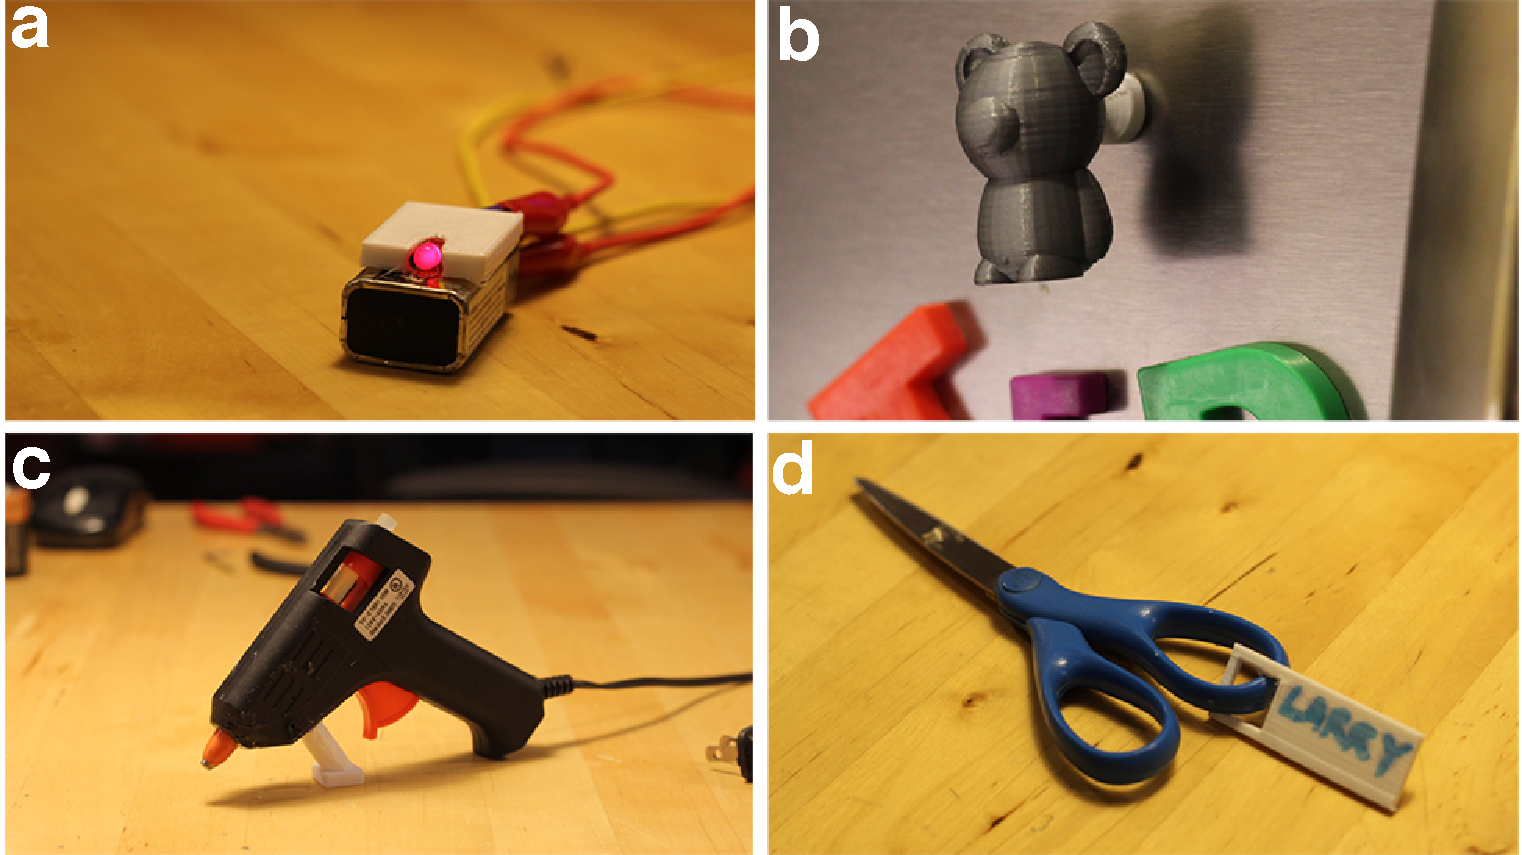
\includegraphics[width=0.8\textwidth]{figures/encore_overview.pdf}
  \caption{Examples of how existing objects can be augmented using our techniques: a) turning a battery into a LED torch; b) making a magnet from a Teddy bear; c) adding a stand to a glue gun and d) attaching a name tag to a pair of scissors. }~\label{fig:encore_overview}
\end{figure*}


These attachment techniques were integrated into Encore--a tool that can import a 3D model of an existing object, perform geometric analyses for the attachment techniques, and allow user exploration through visualization and direct manipulation. Our analysis metrics are designed to provide up-front information about viability, durability and usability of the attachments, where the user can explore tradeoffs among these metrics. Finally, Encore will generate a production-ready model of the parts to be printed, including information necessary for the custom printing process. Figure~\ref{fig:encore_overview} shows an overview of the underlying framework.

\begin{figure*}[h]
  \centering
  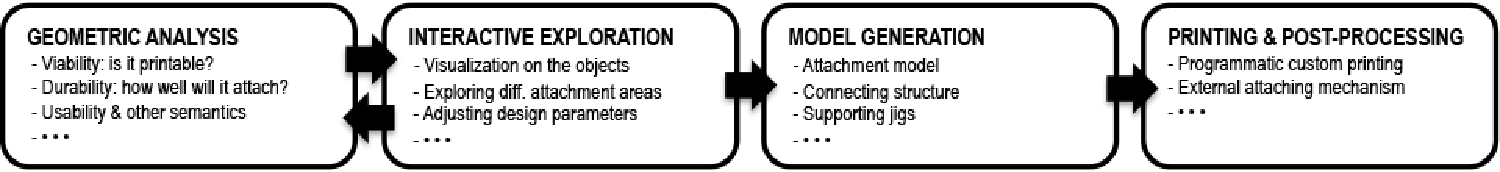
\includegraphics[width=\textwidth]{figures/encore_workflow.pdf}
  \caption{A computational pipeline for designing and fabricating attachments to augment everyday objects. }~\label{fig:encore_workflow}
\end{figure*}

In the remainder of the chapter, I first review existing attachment solutions and how they might afford end-user customization. Then I present the attachment techniques, describe several exemplar analysis metrics for evaluating the goodness of attachment, and present Encore's visualization and direct manipulation interface. Finally I report an evaluation of printing cost and strength.


\section{Existing Attachment Solutions}
Attachment--fastening or otherwise binding two objects together--is a task that commonly arises in everyday life, and one that is not entirely straightforward. Material properties, strength, usability, and aesthetics all need to be considered when attaching objects together. To address this, websites like ThisToThat \footnote{\url{http://www.thistothat.com/}} let a person enter two materials and suggests the best option for gluing them together. Other approaches leverage objects' mechanical properties, such as the widely used joineries and fasteners commonly used in various manufacture industries (e.g., \cite{barrett1990fastener}). Attachment can also be made complex by the specific constraints of the objects being connected. For example, the free universal construction kit\footnote{\url{http://fffff.at/free-universal-construction-kit}} offers adaptors between 10 otherwise incompatible children's construction kits from Lego™ to Tinker toys.

In this work, we are primarily interested in attaching 3D printed components to existing objects. We assume that the existing object is not designed with attachment in mind, and is not to be directly modified (e.g., by drilling holes in order to use a bolt). Specifically, given an existing object and a new part we would like to fabricate and attach, we can either create a binding force between the new part and the old (such as using adhesives, or printing directly over a material that the filament will easily adhere to it) or in some cases we can loosely interlock the new part and the old (such as a buckling a strap through a handle or adding a charm to a charm bracelet or a key to a ring).

Choosing among these forms of attachment is a matter of understanding the task to be accomplished and the constraints that come with it. For example, if we wish to add a doggie bag holder to a dog leash, we may want it to be removable, but not moveable once attached (so it doesn't flap around too much). It must be sturdy enough to survive many walks, dropped leashes, and so on, but does not need to carry much weight (just a roll of plastic bags). It may need to attach just below the handle of a cloth leash, or perhaps we are designing one that can attach to the plastic handle of a retractable leash. As another example, if we wish to add a handle to an espresso cup, it should withstand sheer forces based on the typical weight of a cup. These examples clearly demonstrate the wide range of issues that must be considered, and the interaction of properties of the existing object, task, and object to be attached.

To summarize, to determine the goodness of an attachment technique, viability, durability and usability are all important, although their relative importance may vary. Keeping these issues in mind, our focus in this project is on attachments to, around, or through an existing object without modification by leveraging the fabrication process and customizability of 3D printing. Below I showcase three exemplary attachment techniques.

\section{Techniques For 3D Printed Attachment}
Our techniques allow attachments to be printed directly onto an existing object (print-over), or separately and then adhered or strapped to it (print-to-affix), or through and around the object's holes (print-through). Here we assume that the models of the existing and the new objects have been acquired using 3D scanning, or created from scratch, and focus on methods for attaching the two together.

\subsection{Technique \#1: Print-Over}
The first technique, print-over, is able to print an attachment directly onto the existing object. Once the attachment location is specified, the existing object is oriented and scaffolded with support structures so that it will not move while the attachment is printed on it. It is also important to ensure that the existing object will not impede the motion of the print head while the attachment is being printed.

Figure~\ref{fig:encore_overview}b shows a magnet holder directly printed over a Teddy bear toy (in this case also 3D printed) to make it a fridge magnet. As shown in Figure~\ref{fig:encore_techniques}a, this was done by scaffolding the Teddy bear to the print bed so that the attachment area is facing upward and is accessible by the extruder, which then prints the magnet holder.

\begin{figure*}[h]
  \centering
  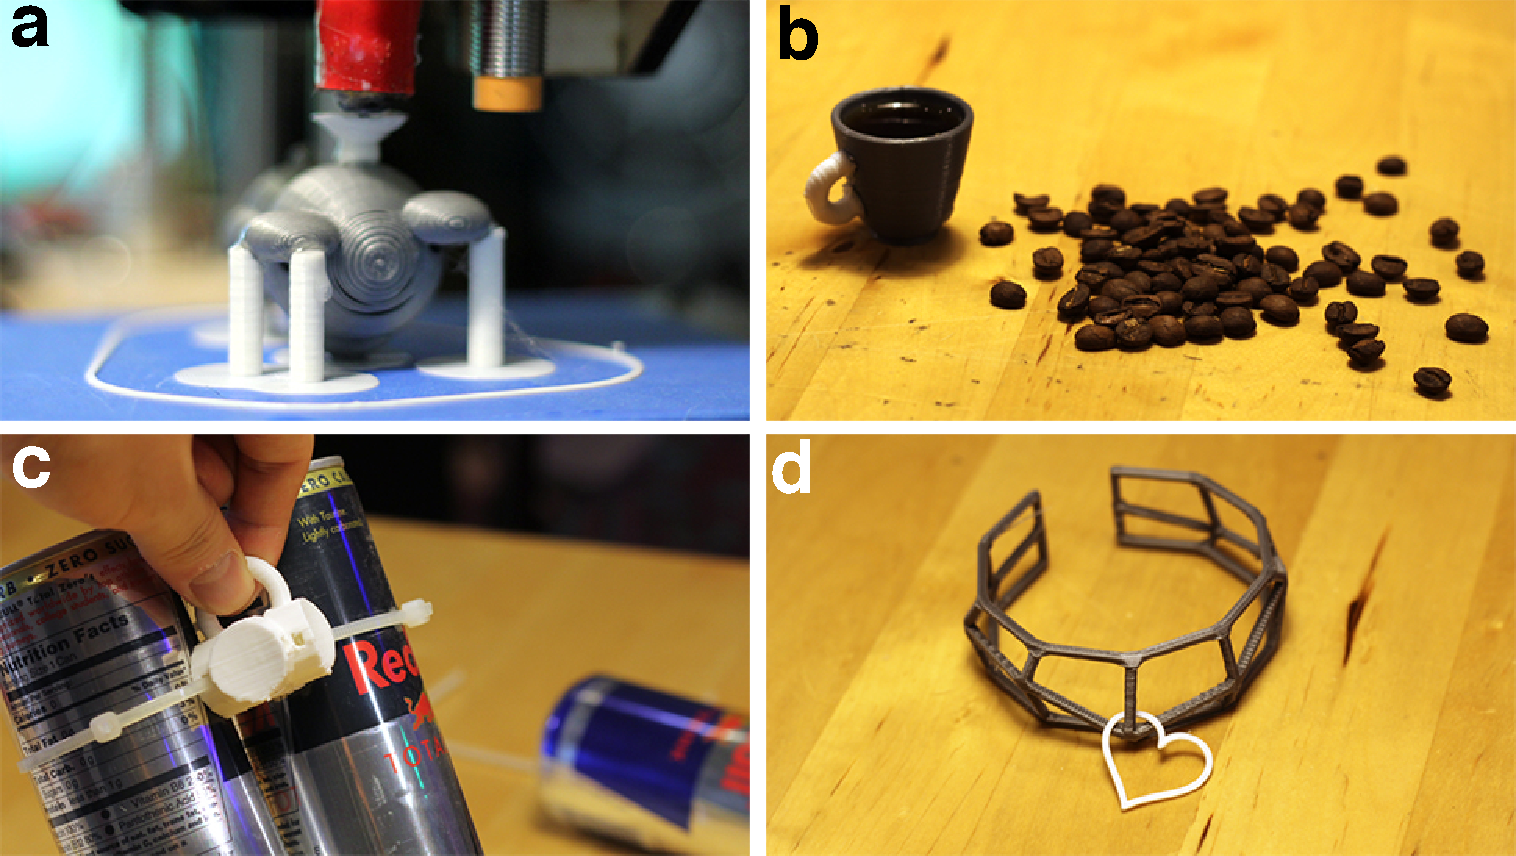
\includegraphics[width=0.8\textwidth]{figures/encore_techniques.pdf}
  \caption{a) The magnet holder printed directly on a teddy bear that was scaffolded on support structures; b) a handle added to an espresso cup; c) strapping to make a reusable “4 pack” handle; and d) a bracelet printed through a heartshaped charm. }~\label{fig:encore_techniques}
\end{figure*}

Print-over works well when the attachment and the existing object are made of the same material, or materials that share similar thermodynamic properties. As detailed later, our evaluation shows that print-over is strong enough to sustain stress as if they had been printed in one piece. When objects are made of less compatible materials, we employ a work-around to perform print-over. Figure~\ref{fig:encore_overview}a shows an LED casing printed directly over a 9V battery to make a simple torch. This was done by adding a thin layer of glue on the battery prior to printing the casing. The glue simply creates a plastic-like layer that allows the printer's material (PLA) to stick to the battery while being printed.

\subsection{Technique \#2: Print-to-Affix}
The second technique, print-to-affix, makes use of the concept of a connector that confomrs to the surface geometry of the existing object and is snug-fit to the new object. This connecter can be printed separately and then attached using external mechanisms (e.g., glue, or straps). This leverages the customizability of 3D printing to bridge objects and attachments that by default are likely to have unmatching surfacing. Figure~\ref{fig:encore_techniques}c shows connectors used for the handle attachment to hold it tight with cans. Print-to-affix is a very general technique and can encompass for example the use of adhesive, straps, or even a custom printed part that snaps into place in some way. It also has the advantage of not preferring the existing object to be flat, as there is no concern about the print head colliding with the existing object.

Figure 1c shows a structure added to a glue gun to make it stand. This geometry was made to precisely match the attaching part on the glue gun, then 3D printed, and attached using adhesive. However, one disadvantage of using adhesive (or the aforementioned print-over) is the difficulty in detaching the attachment for redesign or reuse. Affixing with straps solves this problem. For example, using straps for the `4 pack' holder in Figure~\ref{fig:encore_techniques}c makes this handle reusable without either breaking it or the cans it holds.

Print-to-affix includes a wide variety of options. Details such as whether adhesives or straps are used significantly change the properties of the resulting attachment. For example, in one experiment, a 150mm zip tie could sustain up to a 4kg pulling force before the test object slipped, while the particular adhesive we applied tended to break at a less than 1kg force. On the other hand, using adhesives is less noticeable from an aesthetic standpoint.

\subsection{Technique \#3: Print-through}
The third technique, print through, leverages the structural holes in some existing objects (e.g., keys and rings) to print the attachment through and around it. To accomplish this, the attachment is partially printed, the existing object is placed, and then printing continues until the two objects are interlocked and the print is complete. This requires determining whether there is a viable point at which to stop the print, and whether once the existing object is placed it will interfere with the print head.

Figure~\ref{fig:encore_overview}d shows a name tag printed through the handle of a pair of scissors. As shown in Figure~\ref{fig:encore_printthru}, this was done by programmatically pausing the printer at a point where the scissors can be placed down and out of the way of the print head. Print-through has aesthetic qualities that distinguish it from print-to-affix and print-over: it typically creates a loose but permanent connection between two objects. Figure~\ref{fig:encore_techniques}d is another such example whereby a bracelet was printed through a charm.

\begin{figure*}[h]
  \centering
  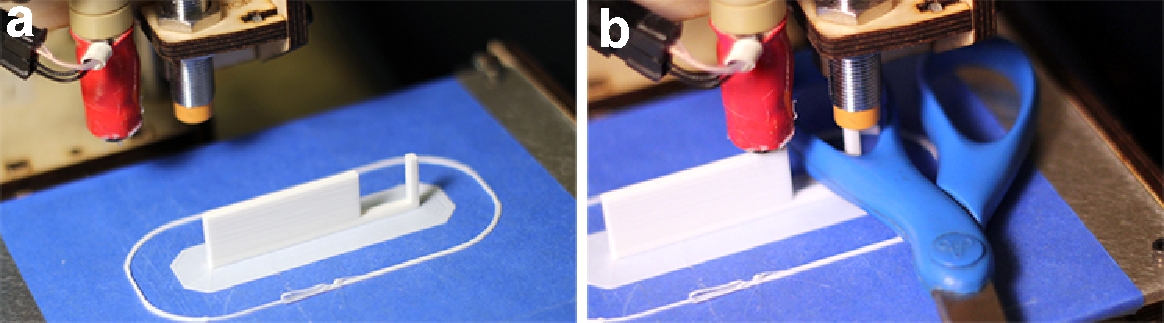
\includegraphics[width=0.8\textwidth]{figures/encore-printthru.pdf}
  \caption{Example of a print-through process: the printer pauses at a point where the scissors can be dropped to interlock with the name tag, after which the print job resumes. }~\label{fig:encore_printthru}
\end{figure*}

As highlighted in the techniques just presented, a range of tradeoffs must be considered when creating 3D printed attachments to existing objects. To address this, we present a series of analysis, based on the geometric properties calculated over the triangular meshes representing the existing object and the attachment. These analyses represent a sample of metrics that pertain to viability, durability, and usability. However, it is our intent and expectation that this set would be expanded over time and as new attachment techniques are explored.

\begin{itemize}
	\item \textit{Viability} indicates whether it is possible for a new part to be fabricated and attached at a given location on an existing object. For example, collision with the extruder during a direct print over process would violate viability;
	\item \textit{Durability} examines how the geometric properties of the contact area between the attachment and the object could potentially strengthen or weaken the bond between them;
	\item \textit{Usability and other semantics} considers various issues related to the actual usage of the attachment, such as the forces we expect to be applied to it, its balance, and some technique-specific issues (such as the length of strap required for fastening an attachment).
\end{itemize}

The next section will describe the details of these analyses, which serve as the computational backend of Encore---an interactive tool that informs people how attachments can be added to existing objects and how well they will perform in terms of viability, durability, usability and other semantics.


\section{Geometric Analysis: Viability}
Viability can encompass issues such as appropriateness for a specific printer with regard to issues such as support or size, as well as feasibility of printing without collision when an existing object is present during printing. Our work focuses on this last issue, which arises during print-over and print-through.
More specifically, when printing involves two objects, it is only viable if {\em (i)} the attachment can be printed without the extruder's tool paths colliding with the existing object (extruder-object collision); {\em (ii)} the attachment and the existing objects also do not intersect and collide with each other for a given spatial configuration (object-object collision). As shown in this section, both types of collisions are affected by the position and orientation of the existing object and the attachment. Thus, we must determine a position and orientation of both objects where the attachment can be printed collision-free.

\subsection{Understanding Viability: Collision Detection}
The first step of viability analysis is to detect collisions that will prevent the attachment from being printed.

\subsubsection{Detecting Extruder-Object Collision}
Extruder-object collision occurs when the placement of the existing object impedes the printer's extruder movement while the attachment is being printed. This type of collision problem is very common in subtractive manufacturing and is often solved by careful tool path planning \cite{chih1998new, lin1996efficient}, such as controlling the path of the cutting bit on a CNC router to avoid running into parts that are not to be removed. WirePrint has shown that collision can be avoided in non-layered additive manufacturing by modeling and considering the geometry of the extruder and the object \cite{mueller2014wireprint}. In print-over, given an attachment $\Lambda$ to an existing object $\Omega$, we scan all $\Omega$'s' vertices above the attaching point to detect whether they are within the range of the extruder's movement, which can be obtained by computing the bounding radii of both the extruder and $\Lambda$.

\subsubsection{Detecting Object-Object Collision}
We consider and address two forms of object-object collision between an attachment and an existing object.

\textbf{Direct Collision}. In an interface for attachment placement, the mapping of the 3D scene onto a 2D screen could cause user errors in the placement of $\Lambda$ with respect to $\Omega$. A user might perceive $\Lambda$ as interlocking with $\Omega$, and yet the two in fact slightly intersect with each other, such that $\Lambda$ is unable to be fabricated (Figure~\ref{fig:encore_feedback}).

\begin{figure*}[h]
  \centering
  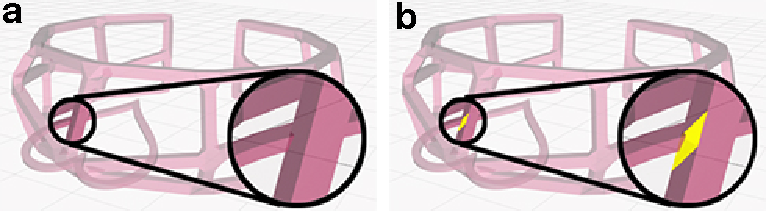
\includegraphics[width=0.75\textwidth]{figures/encore_feedback.pdf}
  \caption{Print-through provides visual feedback (highlighting intersecting faces) to inform users of object-object collision that might not look obvious from certain viewing angle. }~\label{fig:encore_feedback}
\end{figure*}

Such direct object-object collision is commonly dealt with using approximate models (e.g., checking axis-aligned bounding boxes for collision \cite{bergen1997efficient}). Such models could be problematic for attachments: for example, in print-through, $\Lambda$ and $\Omega$ can be interlocking and collision free even though their bounding boxes do intersect with one another.

To address this, we compute whether two objects truly intersect by analyzing their meshes. To narrow down the detection scope, we compute both $\Lambda$ and $\Omega$'s bounding spheres and locate a set of ‘mutually bounded' faces from $\Omega$, denoted as $F^\Omega$. Essentially, $\Lambda$ and $\Omega$ are intersection free if and only if none of $F^\Omega$'s faces intersect with $\Lambda$'s. By walking through a pre-computed octree of $\Lambda$ \cite{meagher1980octree}, we can determine if a given face of $F^\Omega$ intersects with $\Lambda$. Further, as detailed later, we can also visualize the intersecting areas to inform the users how to reposition the attachment to an occlusion-free location (Figure~\ref{fig:encore_feedback}).

\textbf{Indirect Collision}. When objects need to be placed around or through another object (e.g., a partial print), indirect collisions can occur. For example, viability is violated in print-through if one object cannot be moved to its intended interlocked position without ‘passing through' (i.e., intersecting) the body of the other object.

Figure~\ref{fig:encore_interlockable} shows an artificial print-through example to explain this problem. In Figure~\ref{fig:encore_interlockable}a, the existing object (the torus) cannot be inserted into the larger structure (building layer by layer in the direction of the arrow) no matter when the printer is paused. Note that as illustrated in Figure~\ref{fig:encore_interlockable}b, indirect collision is orientation dependent – there might exist an orientation that does provide a viable print for some pause point, different than the one specified by the user for analysis.

\begin{figure*}[h]
  \centering
  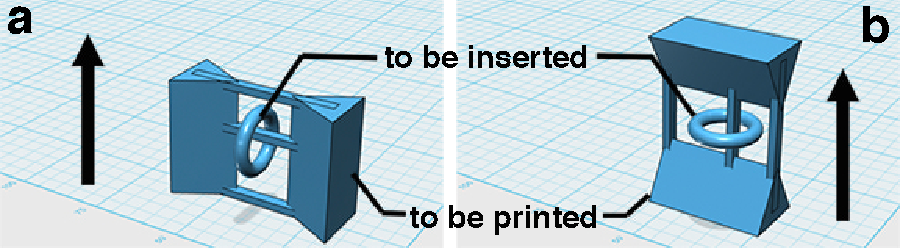
\includegraphics[width=0.75\textwidth]{figures/encore_interlockable.pdf}
  \caption{Interlocking objects are not always viable for printing: a) the torus cannot be inserted while the structure is being printed due to collision; b) a different orientation makes the print viable. (arrows indicate printing directions).}~\label{fig:encore_interlockable}
\end{figure*}

Inspired by Zhou et al.'s use of physics to unfold an object so as to test whether it can be folded \cite{zhou2014boxelization}, we make use of a reverse physics simulation. Specifically, we test whether there is a viable path for moving the existing object to its desired location (e.g., the scissors in Figure~\ref{fig:encore_printthru}) partway through the print of the new object. We test such viability by reversing the insertion process. It starts with an object already inserted into the partial print, which is obtained by slicing the whole print so that its top layer is just above the inserted object. Then gravity is reversed. If the object `escapes' under the reversed gravity, there exists a path for it to be inserted back from above and end up at the same placement where the test started.

In cases where this test fails (i.e., the object is trapped in the partial print), we can also perform a binary search to find a viable printing orientation, which we discuss next.

\subsection{Attaining Viability: Resolving Collision}
Once collision is detected, our analysis also searches for a solution by exploring alternate positions and orientations.

\subsubsection{Resolving Extruder-Object Collision}
Extruder-object collision is only an issue when printing an attachment $\Lambda$ after an existing object $\Omega$ has been placed. Given a candidate surface area $S$ of $\Omega$ on which $\Lambda$ is to be printed, the first step is to rotate $\Omega$ so that $S$ is relatively level and facing upward for extruder to print $\Lambda$ on (e.g., the Teddy bear in Figure~\ref{fig:encore_techniques}a). Generally $S$ is not a perfectly flat surface to print on, so our next step raises $\Lambda$'s first printing layer $P_0$ to be above the entire $S$. However, after these two operations, printing $\Lambda$ might still run into object-extruder collision if parts of $\Omega$ are also above $P_0$. To address this issue, we first print a connector on $P_0$--a cylindrical structure that is small enough to be printed without collision. These connectors serve to continue raising the starting layer until $\Lambda$ can be printed collision-free. One potential issue of this approach is the strength of these connectors in supporting $\Lambda$, which we also discuss later in the durability analysis section.
Even with these solutions, some surface areas, such as those with a high convexity, might still be unprintable. As detailed later, our exploration phase (Figure~\ref{fig:encore_workflow}) visualizes this information to guide the user in selecting alternate viable attachment areas.

\subsubsection{Resolving Object-Object Collision}
For object-object collision, a search for the position and orientation of $\Lambda$ can determine whether there is a viable solution (in which the ‘reversed gravity' test succeeds). A simplified example of this situation is shown in Figure~\ref{fig:encore_interlockable}, where rotating $\Lambda$ by 90 degrees resolves the issue.

Formally stated, the goal is to find a pair of rotations $(\alpha, \gamma)$ such that there exists a viable pause point for $R_x(\alpha)R_y(\gamma)\Omega$. ($R_x$ and $R_y$ are rotation matrices around $x$ and $y$ axis, respectively; rotating around $z$ axis would not change the viability). The solution space is naturally continuous: given an pair of viable $(\hat{\alpha}, \hat{\gamma})$, there must also exist intervals $\alpha_l < \hat{\alpha} < \alpha_u$ and $\gamma_l < \hat{\gamma} < \gamma_u$ such that any printing direction in $\{(\alpha, \gamma) | \alpha_l < \alpha < \alpha_u, \gamma_l < \gamma < \gamma_u \}$ is also viable. Our search process is akin to a binary search of such intervals.

To sum up, the viability analyses described above detect collision issues that arise while fabricating the attachment – either with the extruder or the existing objects. To prevent collision, we can orient the object or raise the starting layer. We also show that a collision-free printing orientation belongs to a continuous solution space and can be found via a binary search.

\section{Geometric Analysis: Durability}
Once a new part is viable for fabrication, the next question is its durability: how well it will attach to the existing object. One simple way to measure durability is to consider the contact area $S$ between the existing object and the attachment; however our framework is extensible to other models and methods such as the cross-sectional analysis \cite{umetani2013cross} and Finite Element Method \cite{szabo1991finite}. Specifically, given a candidate contact area $S$, we consider the following metrics.

\subsubsection{Size}
Size can be approximated by summing up the area of each triangle in or intersecting with $S$. To generalize to multiple attachment sizes, we normalize the measurement by the volume V of the attachment. This metric serves as a simple way to capture an approximation of the structural strength of the connection point with respect to the attachment.

\subsubsection{Flatness}
Flatness can be computed by summing up the vertex-wise distance between $S$ on the existing object and the printing layer at the bottom of the attachment. The flatness score is highest when $S$ is perfectly flat (coplanar with P); and lower as $S$ becomes more irregular, meaning the triangles in $S$ have highly variable heights and orientations, or $S$ has an overall higher curvature.

\subsubsection{Direction and Area of Force}
The relationship between force and strength is affected by the type of attachment being used. For example, techniques such as print-over and using adhesives use interfacial bonds, with adherence to both the existing object and the attachment. In contrast, attachment techniques such as strapping create a force that holds the attachment onto the existing object, which can be measured as follows.

Consider an attachment surface $S$ on the existing object for a strap, we compute $S$'s convex hull $ConvHull(S)$ using a Graham scan \cite{graham1972efficient}. For each point p in $S$, we compute its shortest distance to $ConvHull(S)$: if the distance is smaller than a threshold we consider p to be making contact with a strap around $S$. The object is more strappable at $S$ if most of $S$'s points make contact with the strap. A further consideration is contact point distribution: more evenly distributed contacts suggest a more balanced strapping force.

To sum up, durability examines how the geometric properties of the contact area between the attachment and the object could potentially strengthen or weaken the bond between them. Our analysis shows how contact area and size can be used to compute durability (most usefully for adhesion-based attachments) and explores the metric of strappability, which captures the contact area and force associated with a strap.

\section{Geometric Analysis: Usability \& Semantics}
Even for a new part that is viable and durable, there are often further considerations related to the actual usage of the attachment. We provide two exemplar analysis of usability and semantics: {\em (i)} for handle-like attachments, we consider whether its attachment point creates a balance of the entire object when being gripped or held; and to illustrate a metric which is highly specific to one attachment technique {\em (ii)} an aesthetic strap length metric.

It is only natural that the analysis of usability and semantics would be highly specific to the type of attachment being used. For example, Pr\'evost et al. discuss geometric modifications that can achieve balance such that an object will stand without falling \cite{prevost2013make}. Thus, the metrics we present are by no means exhaustive for the usability and semantic aspects of attachments; rather they suggest exemplar analysis that goes beyond the stage of fabrication and considers the effects and tradeoffs for an attachment in use.

\subsubsection{Balance When Holding an Object By the Attachment}
Balance when holding an object by a given attachment can be measured by moment, which indicates the tendency of the held object to rotate under its own weight. For example, as shown in the ‘4 pack' holder in Figure~\ref{fig:encore_techniques}b, if the handle is rotated 90 degrees, it would be more difficult to hold the cans. When there are multiple contact points selected (such as the handle on an espresso cup), we simply sum up the moments of these points before normalization.

\subsubsection{Technique Dependent Usability Analysis: Strap Length}
Some attachment techniques may make use of very specific usability analysis. For example, the length of the strap is directly related to fastener cost and object appearance. In particular, we consider an analysis of strap length for a candidate attachment configuration normalized to a baseline (e.g., the bounding sphere of the existing object). The strap length can be computed from the aforementioned convex hull of the strapping area.

\section{A Pipeline For Printed Attachments}
We have presented a series of geometric analysis that can be used to quantify the goodness of various potential attachment options from the perspective of viability, durability, and usability. As shown in Figure~\ref{fig:encore_workflow}, analysis results can be integrated into a pipeline for supporting iteration, interactive exploration, model generation, printing and post-processing. We illustrate these phases of the pipeline with our implemented tool, Encore.

\subsection{Interactive Exploration}
The interactive exploration phase creates a feedback loop wherein a user can explore different design parameters. Encore provides visualization and direct manipulation techniques to facilitate this process.

\begin{figure*}[h]
  \centering
  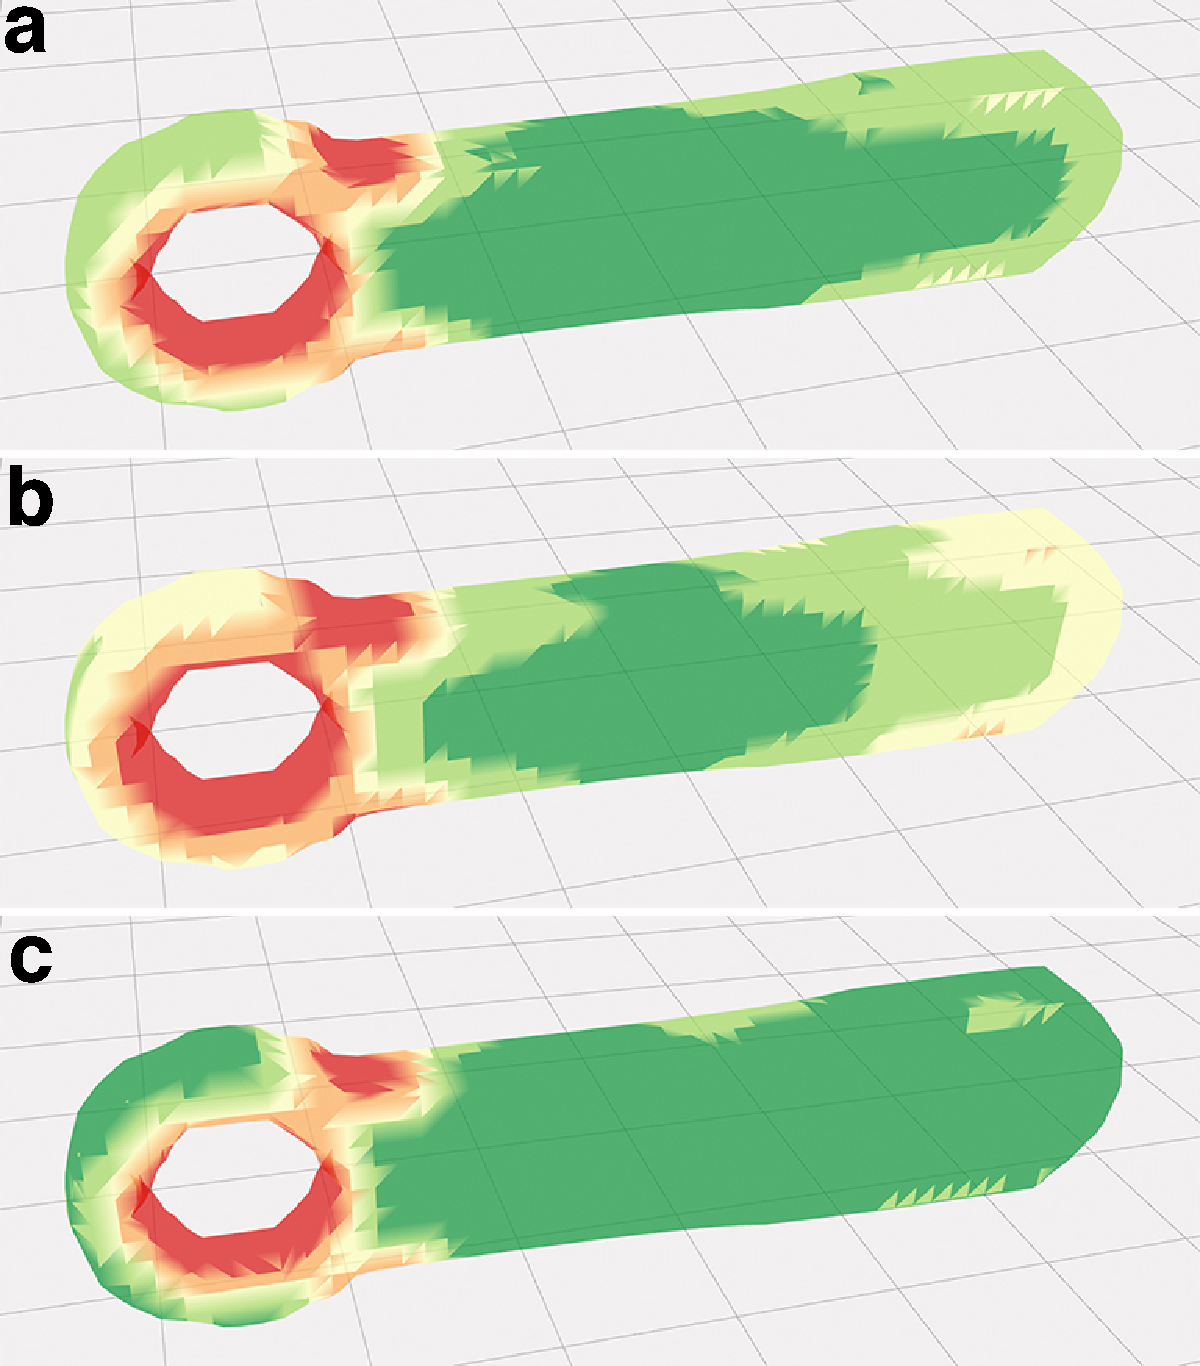
\includegraphics[width=0.6\textwidth]{figures/encore_visualization.pdf}
  \caption{A heat map is an effective way to visualize the analysis results for adding a handle to a wrench: a) red areas indicate a handle cannot be printed over (viability); b) emphasizing durability shows preference for areas with small curvature; and c) emphasizing balance (usability) shows preference for areas near the center of mass (This assumes the forces applied have the same direction as the surface normals).}~\label{fig:encore_visualization}
\end{figure*}

\subsubsection{Visualization Techniques}
Visualization provides effective feedback to the users to inform them about properties of their own design. When making attachments, one type of visualization is to compute an attachment score for each point on an existing object and overlay the results as we render the 3D model. Specifically, for each face on the object's mesh, we locate its neighborhood area $S$, and pre-compute the viability, durability and usability analysis for this area. The results from different analyses can be weighted and combined based on user input and the purpose of the attachment.

Figure~\ref{fig:encore_visualization} shows Encore's heat map visualization of these computed values, rendered on a wrench where the user would like to use print-over to add a handle (e.g., for hanging the wrench from a machine that needs frequent maintenance). The red areas indicate the parts of on the wrench where a handle cannot be printed over due to unavoidable occlusion (Figure~\ref{fig:encore_visualization}a). The user can adjust the weights given to the metrics, such as choosing to emphasize durability. The visualization is interactively updated and shows preference (green) for areas with small curvature (Figure~\ref{fig:encore_visualization}b). Alternatively, the user can emphasize balance, which narrows down the preferred areas to those near the center of mass (Figure~\ref{fig:encore_visualization}c).

\subsubsection{Direct Manipulation Techniques}
Some attachment techniques, such as strapping, might require more user direction. For example, Figure~\ref{fig:encore_feedback} shows in the print-through technique, how the user can position the existing object to interlock with the attachment. When the two meshes intersect with one another, the intersecting area is highlighted, which prompts the user to reposition the object to an intersection free location.
Another useful technique is to allow the user to draw on the existing object to specify the attachment area. For example, for affixing using straps, the user simply draws a stroke around part of the object to indicate a strap. Based on this partial strap, we can find the corresponding cross section by first finding a plane that best fits the stroke points, and then intersecting the object with the plane. Figure~\ref{fig:encore_interaction} shows an example of drawing to specify where to strap an attachment on a bottle.

\begin{figure*}[h]
  \centering
  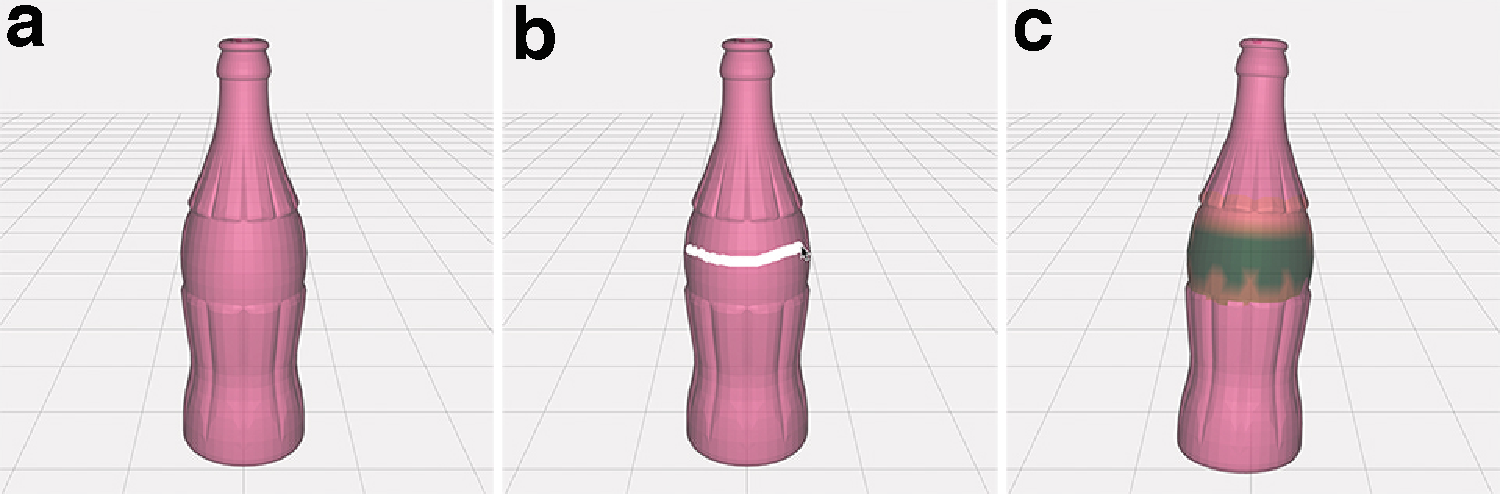
\includegraphics[width=0.8\textwidth]{figures/encore_interaction.pdf}
  \caption{Directly drawing on the object is a simple way to specify the attachment area, such as drawing a stroke around a bottle (a, b) to indicate where to attachment a strap. (c) a heat map visualization around the selected cross section. }~\label{fig:encore_interaction}
\end{figure*}

\subsection{Model Generation, Printing and Post-processing}
Once the user is satisfied with the attachment location, the pipeline continues to the last two phases: model generation, and printing and post-processing.

\subsubsection{Model Generation}
Model generation outputs a single file that includes the attachment, connector(s) and support structure. In particular, as discussed earlier, the connectors can raise the starting layer for printing the attachment to avoid potential occlusion issues; or be designed to snug-fit the existing objects (thus enabling affixing using adhesives or straps).

For some techniques, adding support can also solve occlusion problems. For example, in the print-through technique, when the attachment is much smaller than the existing object, it needs to be raised by a support structure so that the object can go through it while staying below the extruder. Other techniques use support to hold an object in place, such as direct print-over.

Figure~\ref{fig:encore_support}a shows a connector and the support structure for printing over a magnet holder on a Teddy bear (the same one shown in Figure~\ref{fig:encore_techniques}a). In this case, the five support cylinders at the bottom hold the bear in place and at the right orientation and have been prepared to exactly conform to the surface of the bear.

\begin{figure*}[h]
  \centering
  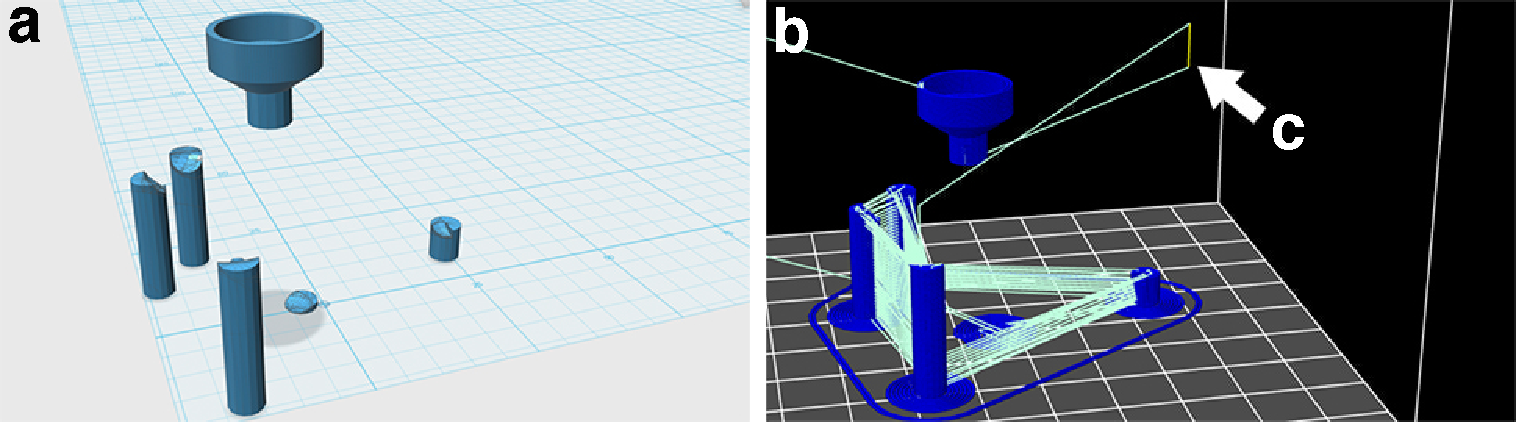
\includegraphics[width=0.9\textwidth]{figures/encore_support.pdf}
  \caption{In the Teddy bear magnet example, a) a model is generated with a magnet holder, a connector, and the support structure; b) Tool path view in Repetier-Host: the extruder pauses and moves away for inserting the teddy bear (c).}~\label{fig:encore_support}
\end{figure*}

\subsubsection{Printing and Post-Processing}
In the last phase, the user imports the generated models into the 3D printing tool chain for fabrication. Some attachment techniques require a simple customization of the printing process, which can be programmatically achieved using 3D printing software such as Repetier-Host\footnote{\url{http://www.repetier.com/
 }} (Figure~\ref{fig:encore_support}b). For example, both print-over and print-through require pausing the printer, inserting the existing object, and then resuming the print job. Having computed the pause point in the analysis, we can generate commands to perform these operations, such as:

\begin{verbatim}

G1 X0 Y0	; move the extruder away
G1 Z40		; raise the extruder
@pause		; pause the print for insertion
; print is manually resumed here after insertion
G1 Z31.550	; restore extruder's height

\end{verbatim}

Figure~\ref{fig:encore_support}c shows the extruder's tool path as a result of these few extra commands. The extruder makes room for the Teddy bear to be positioned onto the support structures. It then returns and finishes printing the magnet holder.

Finally, some techniques require a few post-processing steps after the attachment is fabricated, such as applying adhesives or straps to affix a new part that is printed separately from the existing object.

\subsection{Software and Hardware Implementation}
We have applied a computational framework--geometric analysis, interactive exploration, model generation, printing and post-processing supporting all three attachment techniques in Encore. Encore was implemented in JavaScript primarily using three.js\footnote{\url{http://threejs.org/}}--a library for programming with WebGL. All the attachment examples were fabricated by an FDM printer made from Printrbot's Simple Maker's Kit\footnote{\url{http://printrbot.com/shop/simple-makers-kit-2/}} . We used Slic3r\footnote{\url{http://slic3r.org/
 }} for G-code generation, Repetier-Host for communicating with the printer, and 1.75mm PLA as printing material in all our examples.

\section{Evaluation}
Below we report on an evaluation of our attachment approach from two perspectives: {\em (i)} to evaluate the printing process, we compare the cost of time and material for each technique; {\em (ii)} to evaluate the reliability of the printing results, we tested print-over and print-to-affix techniques, which rely on extrinsic adhesion ir fastening. Specifically, for these techniques, we investigate how well a fabricated handle can sustain forces that typically occur when holding, carrying and controlling an object.

\subsection{Evaluating Time and Material Cost}
One potential benefit of printing to augment existing objects rather than creating new ones is to spend less time and material printing. To verify this, we compare the printing plus processing time and material cost between our attachment techniques (print-over, print-to-affix, print-through) and a baseline approach, which prints a brand new object that has the attachment as an integral part of it.

\subsubsection{Cost Prediction Model}
As shown in Table 1 and Table 2, by the nature of different attachment techniques, we can predict how they differ in printing time and material cost.

Printing time is broken down to time spent on actual 3D printing (T) and time on handling or post-processing (t). For example, print-over requires the printing of the attachment, connector(s), and support structure; it also takes time to insert the existing object to be printed over, as well as to apply adhesives to increase the firmness of the scaffolding.

Material cost is split between printing the attachment and other structures. For example, print-through might also require support structures to keep the interlocking object collision free, even if the attachment itself does not have overhang problems.
For the baseline technique, printing time and material is spent on a new object made of the original object combined with the added attachment.

\begin{table}[h!]
\small
\centering
\caption{Prediction models for printing time of attachment techniques and data from a exemplar object+attachment. }
\label{tbl:encore_predtime}
\begin{tabular}{| c | c | C{9cm} | c |}
\hline
\multicolumn{2}{|c|}{\textbf{Technique}}   & \textbf{Prediction model for time}                                                & \textbf{\begin{tabular}[c]{@{}c@{}}Case study: \\ Utah teapot\end{tabular}} \\ \hline
\multicolumn{2}{|c|}{Print-over}           & $T_{attachment} + T_{connector} + T_{support} + t_{insert} + t_{apply\_adhesive}$ & 31:41                                                                       \\ \hline
Print-to-Affix & Adhesive & $T_{attachment} + t_{apply\_adhesive}$                                            & 13:56                                                                       \\ \cline{2-4}
                                & Strap    & $T_{attachment} + t_{strap}$                                                      & 11:27                                                                       \\ \hline
\multicolumn{2}{|c|}{Print-through}        & $T_{attachment} + t_{insert}$                                                     & 19:43                                                                       \\ \hline
\multicolumn{2}{|c|}{Print as one piece}   & $T_{attachment+object}$                                                           & 1:13:13                                                                     \\ \hline
\end{tabular}
\end{table}

\begin{table}[h!]
\small
\centering
\caption{Prediction models for material cost of attachment techniques and data from a exemplar object+attachment.}
\label{tbl:encore_predmat}
\begin{tabular}{| c | c | C{9cm} | c |}
\hline
\multicolumn{2}{|c|}{\textbf{Technique}}   & \textbf{Prediction model for time}                                                & \textbf{\begin{tabular}[c]{@{}c@{}}Case study: \\ Utah teapot\end{tabular}} \\ \hline
\multicolumn{2}{|c|}{Print-over}           & $M_{attachment} + M_{connector} + M_{support}$ & 916mm                                                                      \\ \hline
Print-to-Affix & Adhesive & $M_{attachment}$                                            & 402mm                                                                       \\ \cline{2-4}
                                & Strap    & $M_{attachment}$                                                      & 396mm                                                                     \\ \hline
\multicolumn{2}{|c|}{Print-through}        & $M_{attachment} + M_{support}$                                                     & 582mm                                                                      \\ \hline
\multicolumn{2}{|c|}{Print as one piece}   & $M_{attachment+object}$                                                           & 3054mm \\ \hline
\end{tabular}
\end{table}

\subsubsection{A Case Study}
We verify these intuitions in a concrete attachment case: adding a torus-shaped handle to the Utah teapot. We chose the Utah teapot because it is a classic 3D model and because it is also one of the few widely used 3D models where all of our techniques are applicable. The results are shown in Table~\ref{tbl:encore_predtime} and Table~\ref{tbl:encore_predmat}.

The goal of this evaluation is to reveal how time and cost differ between various techniques, rather than to obtain a `true' value through repetitive trials. As such, we used the slicer program (Slic3r) to estimate printing time and material cost. This program calculates time and cost as it analyzes the input models and generates the corresponding G-code. For techniques that require handling or post-processing, such as applying adhesive, we empirically estimate the time. The particular adhesive we chose (Loctite “Professional Heavy Duty” Epoxy Loctite \#1172794 requires 5 minutes of `setting' time, while strapping usually takes no longer than 3 minutes.

Both the prediction model and case study results support our intuition--when support is needed, time and materials go up; and the baseline condition is dominated by the time needed to print the existing object.

To better understand the tradeoffs, we conducted another evaluation to test the general strength of our print-over and print-to-affix, also compared to the same baseline (an integral print of existing object and attachment). Print-through is often done loosely without binding between surfaces. Thus strength issues for print-through are directly related to the objects themselves, rather than the attachment technique. Similarly, print-to-affix using adhesives depends heavily on properties of the adhesive used. As such, no testing was performed for these two techniques. We report on print-over and print-to-affix using strapping.

\subsection{Evaluating Strength of Printed Attachments}
The goal of this evaluation is to understand the tradeoffs and limits of our techniques in comparison to each other. We tested a type of attachment – handles, as they are likely to experience external forces, such as holding, gripping or pulling. For each attachment technique tested, we fabricated handles using the same printer and material as described earlier. Similar to \cite{umetani2013cross}'s test of printed objects' cross sectional strength, we exerted a bending force tangential to each handle's attachment point (pulling the handle sideways at $90^{\circ}$ with respect to its main axis, as illustrated in Figure~\ref{fig:encore_eval_scene}). We then gradually increased the force and measured the point of fracture \cite{tetelman1967fracture}.

\subsubsection{Evaluating Print-Over Attachment}
For testing print-over attachment, we designed a torus-shaped handle with fixed outer radius of 7.5 mm and inner radius of 2.0 mm. We empirically set these values to match the size of human fingers. Larger scales of handles are much more time-consuming to fabricate and might go beyond the dimension limit of our printer. Thus we leave them for future work.

We then computationally generated a series of 20mm by 20mm by 5mm platforms whereon to fabricate the torus handles, connected via a cylindrical connector (radii: 1.5mm, height: 3mm).

Next we modified the top surfaces of these platforms: the independent variables are the Curvature and Roughness of these top surfaces.

\begin{figure*}[h]
  \centering
  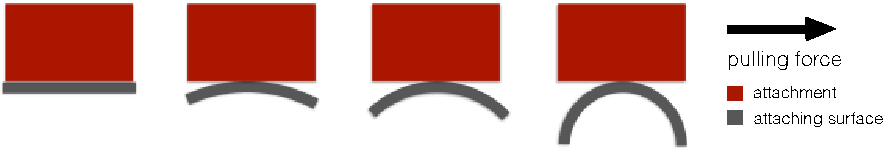
\includegraphics[width=0.9\textwidth]{figures/encore_eval_printover.pdf}
  \caption{To test print-over in comparison to printing in one piece, we used both techniques to print attachments on surfaces with varied curvatures and then exerting tangential pulling force.}~\label{fig:encore_eval_strap}
\end{figure*}

\begin{itemize}
\item Curvature. Assume $R$ is the radius of a platform's top spherical surface and $r$ is the radius of the cylindrical connector of the handle. We modeled the curvature by $C = r/R$. Specifically, we tested on $C$ = 0 (a flat surface), 0.25, 0.5, and 1.

\item Roughness. We performed Boolean subtraction operation between the platform's top surface and a pre-set number $N$ of small spheres whose centroids are on the surface, positions randomized, and radii randomly distributed in [0.25mm, 1mm]. This made the surface porous, thus creating roughness. We tested on $N$ = 0 (smooth surface), and 10 (rough surface).
\end{itemize}

We fabricated the platforms and handles under these conditions using print-over and the baseline print-in-one-piece approach.

As shown in Figure~\ref{fig:encore_eval_scene}, we clamped the platform firmly onto the top of a table so that the handle was pointing upward. We then used a handheld scale to hook and pull the handle horizontally. We used a slow uniform motion for increasing the force. The process was videotaped to capture the scale's reading at the moment when the handle fractured or detached. We performed three trials for each condition.

\begin{figure*}[h]
  \centering
  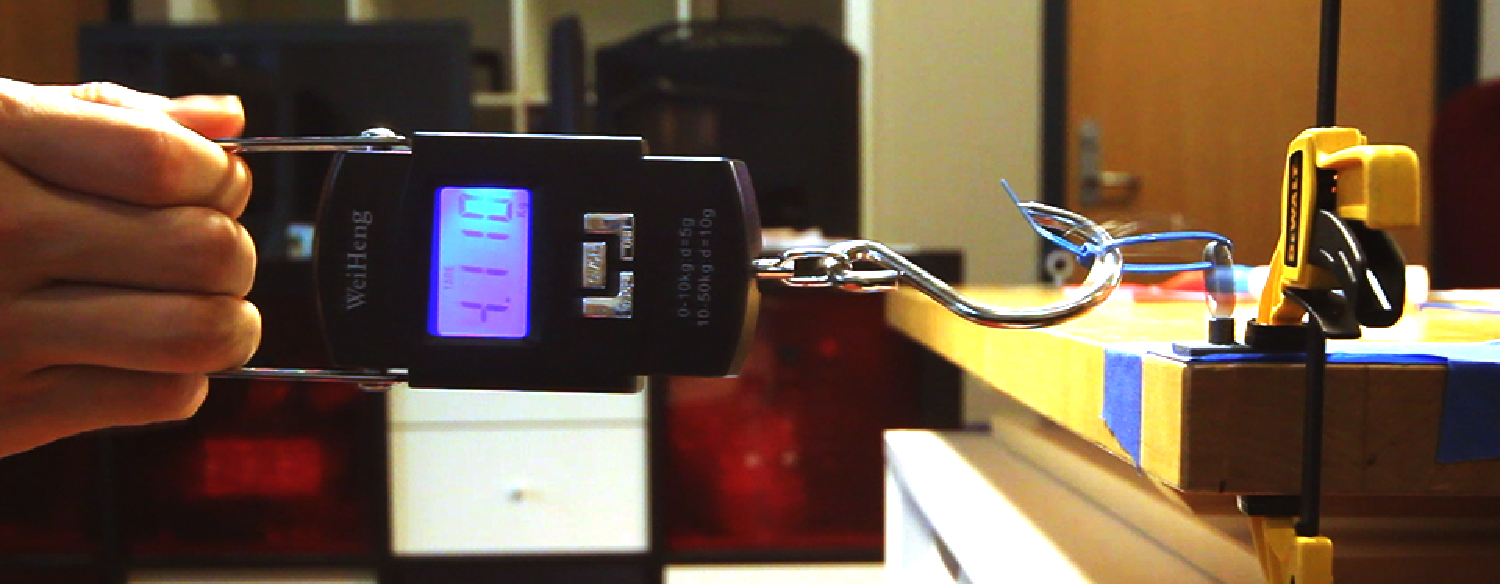
\includegraphics[width=0.9\textwidth]{figures/encore_evaluation_scene.pdf}
  \caption{Testing the strength of a 3D printed handle attachment (b) by clamping it on a table (c) and pulling using a scale to measure force (a).}~\label{fig:encore_eval_scene}
\end{figure*}

Figure~\ref{fig:encore_eval_result} shows the results of the strength test: overall print-over's best performance was close to that of the baseline. However, it suffered from an increase of surface curvature (Figure~\ref{fig:encore_eval_result}a) and roughness (Figure~\ref{fig:encore_eval_result}b).

\begin{figure*}[h]
  \centering
  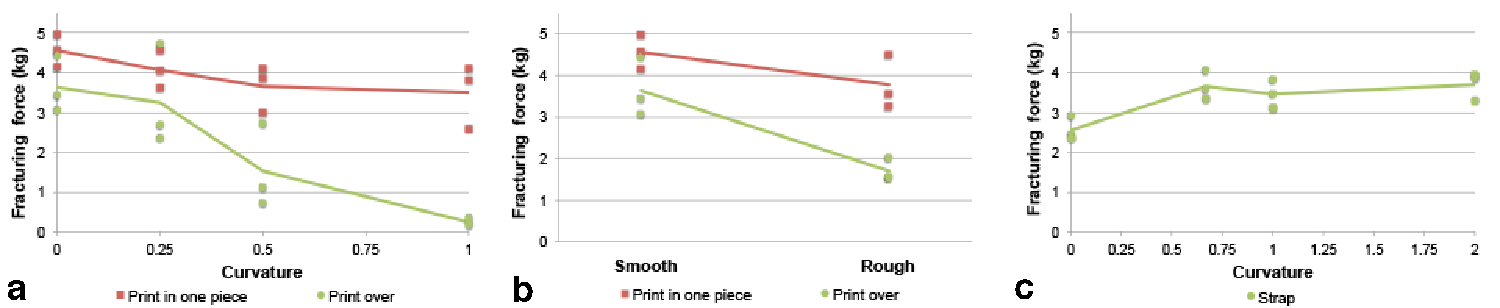
\includegraphics[width=1\textwidth]{figures/encore_evaluation_results.pdf}
  \caption{Strength test results show print-over is strong enough to sustain stress as if they had been printed in one piece. Both our techniques suffer from an increase of surface curvature (a) and roughness (b); (c) shows that affixing with straps (150mm zip tie) is able to sustain over 2.5 kg of pulling, and reacts differently to curvature. }~\label{fig:encore_eval_result}
\end{figure*}


Affixing using adhesion is also related to this evaluation. However, its performance is hard to test in a general way, as it strongly depends on the particular types of adhesives used, as well as the user's experience and expertise of handling it. Therefore we leave it as future work.

\subsubsection{Evaluating Strapping-based Attachment Techniques}
Using straps requires a different analysis than print-over. The key question for strapping is how likely the object is to ‘slip' through the strap when pulling forces are exerted. This is a potential issue that does not occur with the baseline and adhesive attachment mechanisms. Thus we tested this affixing technique independently of the other attachment options.

Specifically, given the same cross section $S$ (we use a circular $S$), we are interested in whether and how the curvature perpendicular to $S$ affects `strappability'. To test this, we computationally generated a series of olive-shaped objects created by revolving a circular segment (with radius $R$) around its secant. We computed the secant so that the revolved shape had a cross section of radius L/2. We then symmetrically cut off the two ends of so that the remaining pieces have a uniform length of $L$.

We quantified curvature as $C = L/R$. We tested $C$ = 0 (a cylindrical lateral area), 0.67, 1, and 2. For each object, we generated a handle attachment using Encore, and then fabricated it and strapped it around the center of the object using a 150mm zip tie. We then firmly clamped the handle to a table and then pulled on the strapped object, measuring the minimal force required to pull the test object out of the strap using a similar setup as the previous test (Figure~\ref{fig:encore_eval_strap}).

\begin{figure*}[h]
  \centering
  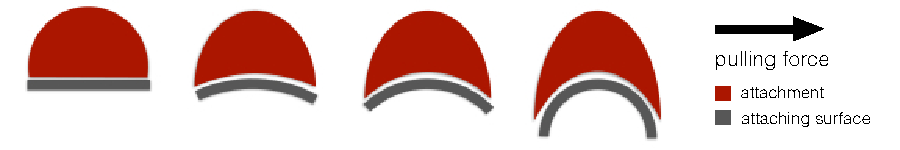
\includegraphics[width=0.9\textwidth]{figures/encore_eval_strap.pdf}
  \caption{To test strapping in print-to-affix, we increased the curvature between the attachment and the attaching surface and exerted tangential pulling force.}~\label{fig:encore_eval_strap}
\end{figure*}

Figure~\ref{fig:encore_eval_result}c shows the test results. Depending on the curvature, a 150mm zip tie attached using our approach can sustain a pulling force of from 2.5 to 4 kg without letting the object slip. Interestingly, strapping strength improved with increased curvature (Figure~\ref{fig:encore_eval_result}c), in contrast to other attachment methods (Figure~\ref{fig:encore_eval_result}a).

\section{Summary of Attachment Techniques}
Although the tested attachment techniques were developed using the same framework, our performance testing demonstrates that they have their own unique advantages and weaknesses. A limitation of our evaluation is its focus on 3D printed existing objects. In this discussion we provide some anecdotal intuition about other factors that might affect the reliability of attachments fabricated by our techniques. Further, to better understand these techniques as a whole, we also discuss some practical issues in comparison with one another.

Print-over, as shown in our evaluation, creates strong adhesion between attachments and objects that are made of the same or very similar material. It also requires no post-processing. However, it has weak adhesion on some materials. For example, when making the LED torch (Figure~\ref{fig:encore_overview}a), our initial attempt to directly print on the metal shell of the battery was not successful. The problem was eventually solved by the simple addition of a thin layer of glue on top of the battery shell. We expect that the use of a glue layer will show promise in other situations as well, but substantially more experimentation and testing is required before its range and properties can be precisely understood.

Affixing with adhesives is widely applicable to a range of geometry and material. But it requires good selection of adhesives, and in some cases careful handling of the amount and mixing of ingredients in order to achieve the best adhesion. Compared with the other techniques (e.g., print-over and print-through), affixing with adhesives relies perhaps the most on the expertise of the users.

Affixing with straps is easily adjustable and also makes an attachment reusable. However, it could be less aesthetically desirable for some use cases. Surprisingly, within the range of our tests, as curvature increased strapping attachment became stronger, whereas all other techniques became weaker. We hypothesize that when the interface between the existing object and the compliant strap has higher curvature, it requires more deformation of the strap in order for the object to slip. Thus the strap can sustain a higher pull force when the curvature increases. However, this hypothesis requires more investigation.

Print-through is a natural attachment mechanism that requires no adhesion or fastening. However, it has limited scope of use as only some objects have appropriate holes or loops that are required to perform this technique.

Despite its increasing popularity, 3D printing has been used almost exclusively to create objects `from scratch', rather than leveraging things that already exist in our day-to-day life. In this project, we present a framework for using 3D printing to augment everyday objects, and provide specific analytical and computational support for realizing one approach of augmentation – adding functional attachments to existing objects. Our framework encompasses key aspects of attachment including geometric analysis, interactive exploration, model generation, and printing and post-processing support. In particular, we present an extensible set of analytical techniques, all based on the geometric form of the existing object and the proposed attachment, and range from very general print viability issues, to durability issues, to very specific usability issues.

There are several remaining questions that require further investigation. Foremost, are there any other attachment techniques that can leverage the use of a 3D printer? Are there any new perspectives that could be introduced into the analyses? Are there any specific use of adding attachments to existing objects that might require further computational support? In my next project, I focus on exploring the third question: I go from developing attachment techniques to enabling the design of functional attachments that can adapt real world objects for custom use.

Another question is given these attachment techniques, how we can design add-on components so that they can serve to augment an object in user-customized ways. My next chapter answers this question through the exploration of designing 3D printed adaptations---components that mechanically enhance or repurpose an existing object.

\chapter{Adapting Real World Objects for Custom Users and Use Cases}

In our everyday life, we often find a need to adapt objects or tools, as the way they were originally designed might not work for certain users or use cases. For example, a faucet might be out of reach for a child, thus it needs to be extended\footnote{\url{http://peachyco.com/handleextender.html}} (Figure~\ref{fig:reprise_existing_adaptations}a); it is hard to hold a drill bit straight while sharpening it, thus a guide comes in handy to keep it in place\footnote{\url{http://www.thingiverse.com/thing:1024834}} (Figure~\ref{fig:reprise_existing_adaptations}b); painting a big surface with a spray-can could be fatiguing for the fingers, thus a mechanism can be used to turn it into a spray-gun\footnote{\url{http://www.thingiverse.com/thing:51966}} (Figure~\ref{fig:reprise_existing_adaptations}c). These add-on components are called \textit{adaptations}. Adaptations change the mechanical properties of existing objects to make them more accessible or to customize them for specific use cases.

The advent of low-cost 3D printing offers the possibility to rapidly construct a wide range of adaptations. However, designing or re-purposing adaptations is hard with general-purpose 3D modeling software, as it requires a certain level of expertise from users \cite{hurst2013making}. In general, 3D modeling tools do not take into account how an object is used, what adaptation strategy is available, or how to rapidly generate the corresponding geometry or further customize it.

Prior work, such as Patching \cite{teibrich2015patching}, Encore \cite{chen2015encore} and AutoConnect \cite{koyama2015autoconnect}, mostly focuses on attaching or directly fabricating new components onto existing objects. However, it remains unclear how to design these components so that they can serve to adapt the objects in user-customized ways. P.Pod \cite{davidoff2011mechanical} and RetroFab \cite{ramaker2015retrofab} explored the mechanical problem of hijacking and automating controls on existing physical interfaces. However, such mechanisms are usually too heavyweight for adapting common household items and hand tools. 

In this chapter, I build on previously explored attachment techniques, and develop a design tool for specifying, generating, customizing and fitting 3D printable adaptations onto everyday objects. My particular focus is on empowering end users to leverage new fabrication technologies to create adaptations by providing high-level techniques for specification and computational support for geometry generation.

Reprise allows a user to specify how an object is used and with what types of action, such as using a virtual hand (Figure~\ref{fig:reprise_teaser}b) to indicate how a person would hold a wire cutter. As 3D geometry itself does not encode how an object is used in the real world, Reprise' techniques enable a user to interactively describe this information \textit{in situ} on models of the objects.

Once the actions are specified, this information is fed into a library of design strategies--Wrapper/Extension, Handle, Lever, Anchor/Stand, and Guide (Figure~\ref{fig:reprise_design_space}). These adaptation strategies were derived from an analysis of over 3000 lifehacking and assistive technology examples found in three books \cite{plaxen2005adapt, willkolmm2013assistive, robitaille2010illustrated} and two online communities \cite{thingiverse,pinterest}. A user can select one or more strategies, which automatically generate the initial design of an adaptation, such as a wrapper for a cutter's handle (Figure~\ref{fig:reprise_teaser}c), levers for easing  clutching operation (Figure~\ref{fig:reprise_teaser}g), or a structure to anchor the cutter for situated use (Figure~\ref{fig:reprise_teaser}i).

To further iterate on the design, a user can manipulate simple slider widgets to customize these adaptations to better suit the person's needs and preferences, such as making the cutter's wrapper longer and thicker for easier gripping (Figure~\ref{fig:reprise_teaser}d), increasing the levers' torque for clutching (Figure~\ref{fig:reprise_teaser}g), or making a larger base for stability (Figure~\ref{fig:reprise_teaser}k). Finally, Reprise also provides a simple toolkit for making the adaptations more attachable onto the objects, such as generating a pipe clamp that connects the cutter's handle to the anchor (Figure~\ref{fig:reprise_teaser}k).

\begin{figure*}
  \centering
  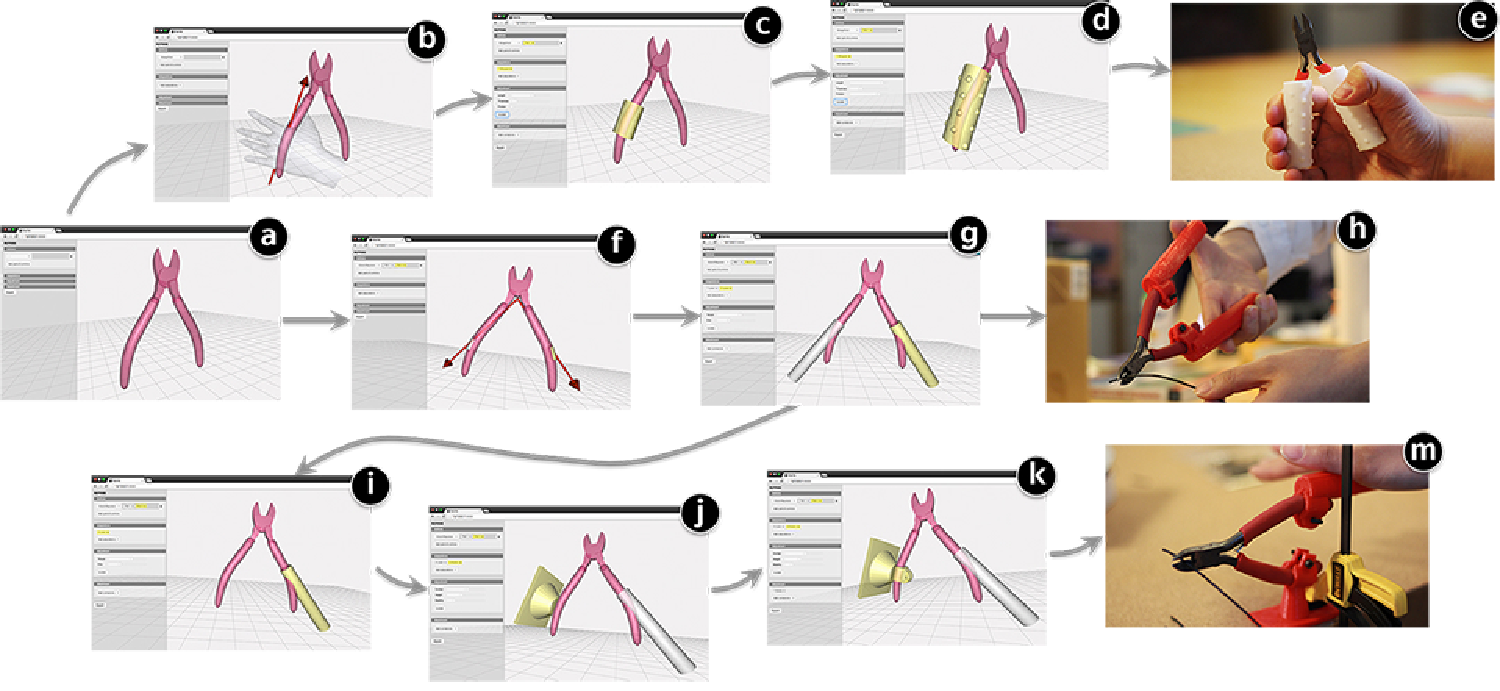
\includegraphics[width=1\textwidth]{figures/reprise_scenarios_v1.pdf}
  \caption{Our main contribution is the tool integration and a formalized design workflow for making 3D printable adaptations onto everyday objects. For example, an occupational therapist can use our tool to explore different strategies of adapting a wire cutter (a), such as creating a wrapper to soften the grip (b-e), adding two levers to assist with clutching (f-h), or replacing one lever with an anchor to situate the cutter on the work surface (i-m).}~\label{fig:reprise_teaser}
\end{figure*}

To demonstrate the expressiveness as well as understanding the limitations of Reprise, we replicated existing adaptation examples found during our design space exploration (Figure~\ref{fig:reprise_design_space}). We identified a real world exemplar for each of 18 cells of the two-dimensional design space. Among the 18 examples, Reprise was able to replicate 15 of them; the other 3 cases suggest new features to be added to the tool and  fertile opportunities for future work.

\begin{figure}[!h]
  \centering
  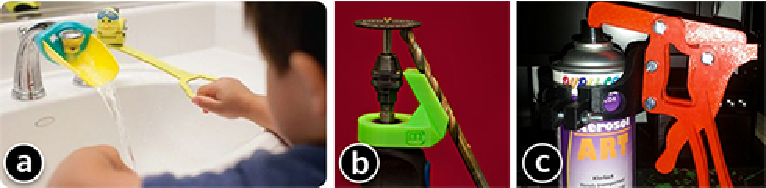
\includegraphics[width=0.7\textwidth]{figures/reprise_existing_adaptations.pdf}
  \caption{Existing examples of adapting everyday objects: a faucet extension (a), a guide for sharpening drill bit (b), and turning a spray-can to a spray-gun (c).}~\label{fig:reprise_existing_adaptations}
\end{figure}

The main contribution of the Reprise tool lies in its ability to generate and iterate across a range of likely useful adaptations. However, it can also be seen as an early exemplar in a class of design tools which can make 3D printing more accessible and useful for ordinary people. In particular, it goes beyond the specification of geometry alone to provide very application domain specific knowledge and features.  This helps to substantially reduce the gulf of execution \cite{norman2013design} that users must bridge as they cross from function to geometry, e.g., from geometric form to the implications of that geometry on the desired end result.

\section{Scenario Walkthrough: Adapting a Cutter}
Reprise lets a user explore a range of design strategies for adapting everyday objects. To set the scene, we first walk through the flow of Reprise in an exemplar scenario where Larry--an occupational therapist--is trying to adapt a wire cutter for an electrician who recently suffered from a hand injury.

\subsection{Iteration I: Generating Wrappers for a Better Grip}
To start, Larry imports a 3D model of the cutter (from a provided repository or through scanning). He selects `Grasp/Hold' as the type of action the patient is having difficulty with. He then clicks on the handle of the cutter to specify the part that is being grasped. Reprise shows a virtual hand model, which Larry can rotate to indicate the relative orientation between the gripping hand and cutter (Figure~\ref{fig:reprise_teaser}b). Next, Larry selects `Wrapper/Extension' as the adaptation strategy. Based on the previously specified grasping action and its hand orientation, the system generates an initial design of the wrapper (Figure~\ref{fig:reprise_teaser}c). Larry wants to further tweak the design using simple slider controls. He adjusts the `Length' slider to make sure the wrapper covers an area large enough for three fingers. He then increases the thickness to make a rounder grip. To further tighten the grip, he adds small bumps to increase the friction (Figure~\ref{fig:reprise_teaser}d). Finally, Larry exports the generated geometry as an STL file and prints the adaptation using a soft material (such as NinjaFlex\footnote{\url{http://www.ninjaflex3d.com/products/ninjaflex-filaments/}}), which provides a soft grip and makes the wrapper snugly fit with the cutter's handle (Figure~\ref{fig:reprise_teaser}e).

\subsection{Iteration II: Making Levers to Assist with Clutching}
Larry's patient responds positively to the soft wrapper. However, while he can now comfortably hold the cutter, his hand is still too weak to perform the necessary clutching action, especially when cutting hard wires. Thus Larry explores an alternate design strategy. In Reprise, he first selects `Clutch/Squeeze' as the target operation. He selects the two handles as the components on which clutching is applied, and then moves the cursor to indicate the fulcrum of clutching. In these few steps, he specifies the two arms for clutching (Figure~\ref{fig:reprise_teaser}f). With this information, Larry proceeds to select `Lever' as the adaptation strategy, which automatically generates two levers from the handles (Figure~\ref{fig:reprise_teaser}g). Larry then tweaks the design, playing with the torque of the levers, as well their size for grasping.

\subsection{Iteration III: Anchoring the Cutter for Situated Use}
Larry's patient does not like the lever design, as it  makes the cutter somewhat too big to hold in one hand (Figure~\ref{fig:reprise_teaser}h). To solve the problem, Larry uses Reprise to replace one lever with an anchoring structure with which he can affix one of the cutter's handles on the work surface (Figure~\ref{fig:reprise_teaser}ij). The patient then simply uses his palm and body weight to press down and cut wires. The key here is to firmly attach the anchor to the cutter's handle. Reprise's attachment toolkit allows Larry to generate a pipe clamp for holding the cutter in place on the anchor (Figure~\ref{fig:reprise_teaser}k). Once printed, Larry bolts the cutter on the anchor, which is then clamped onto the patient's work surface (Figure~\ref{fig:reprise_teaser}m).

To summarize, Reprise allows Larry to generate adaptations with just a few clicks, to tweak the design using simple slider controls, and to explore different design strategies while iterating and customizing the adaptation to suit the patient's particular needs and preferences. Below we describe a design space that informs the design and implementation of Reprise.

\begin{figure*}[!p]
  \centering
  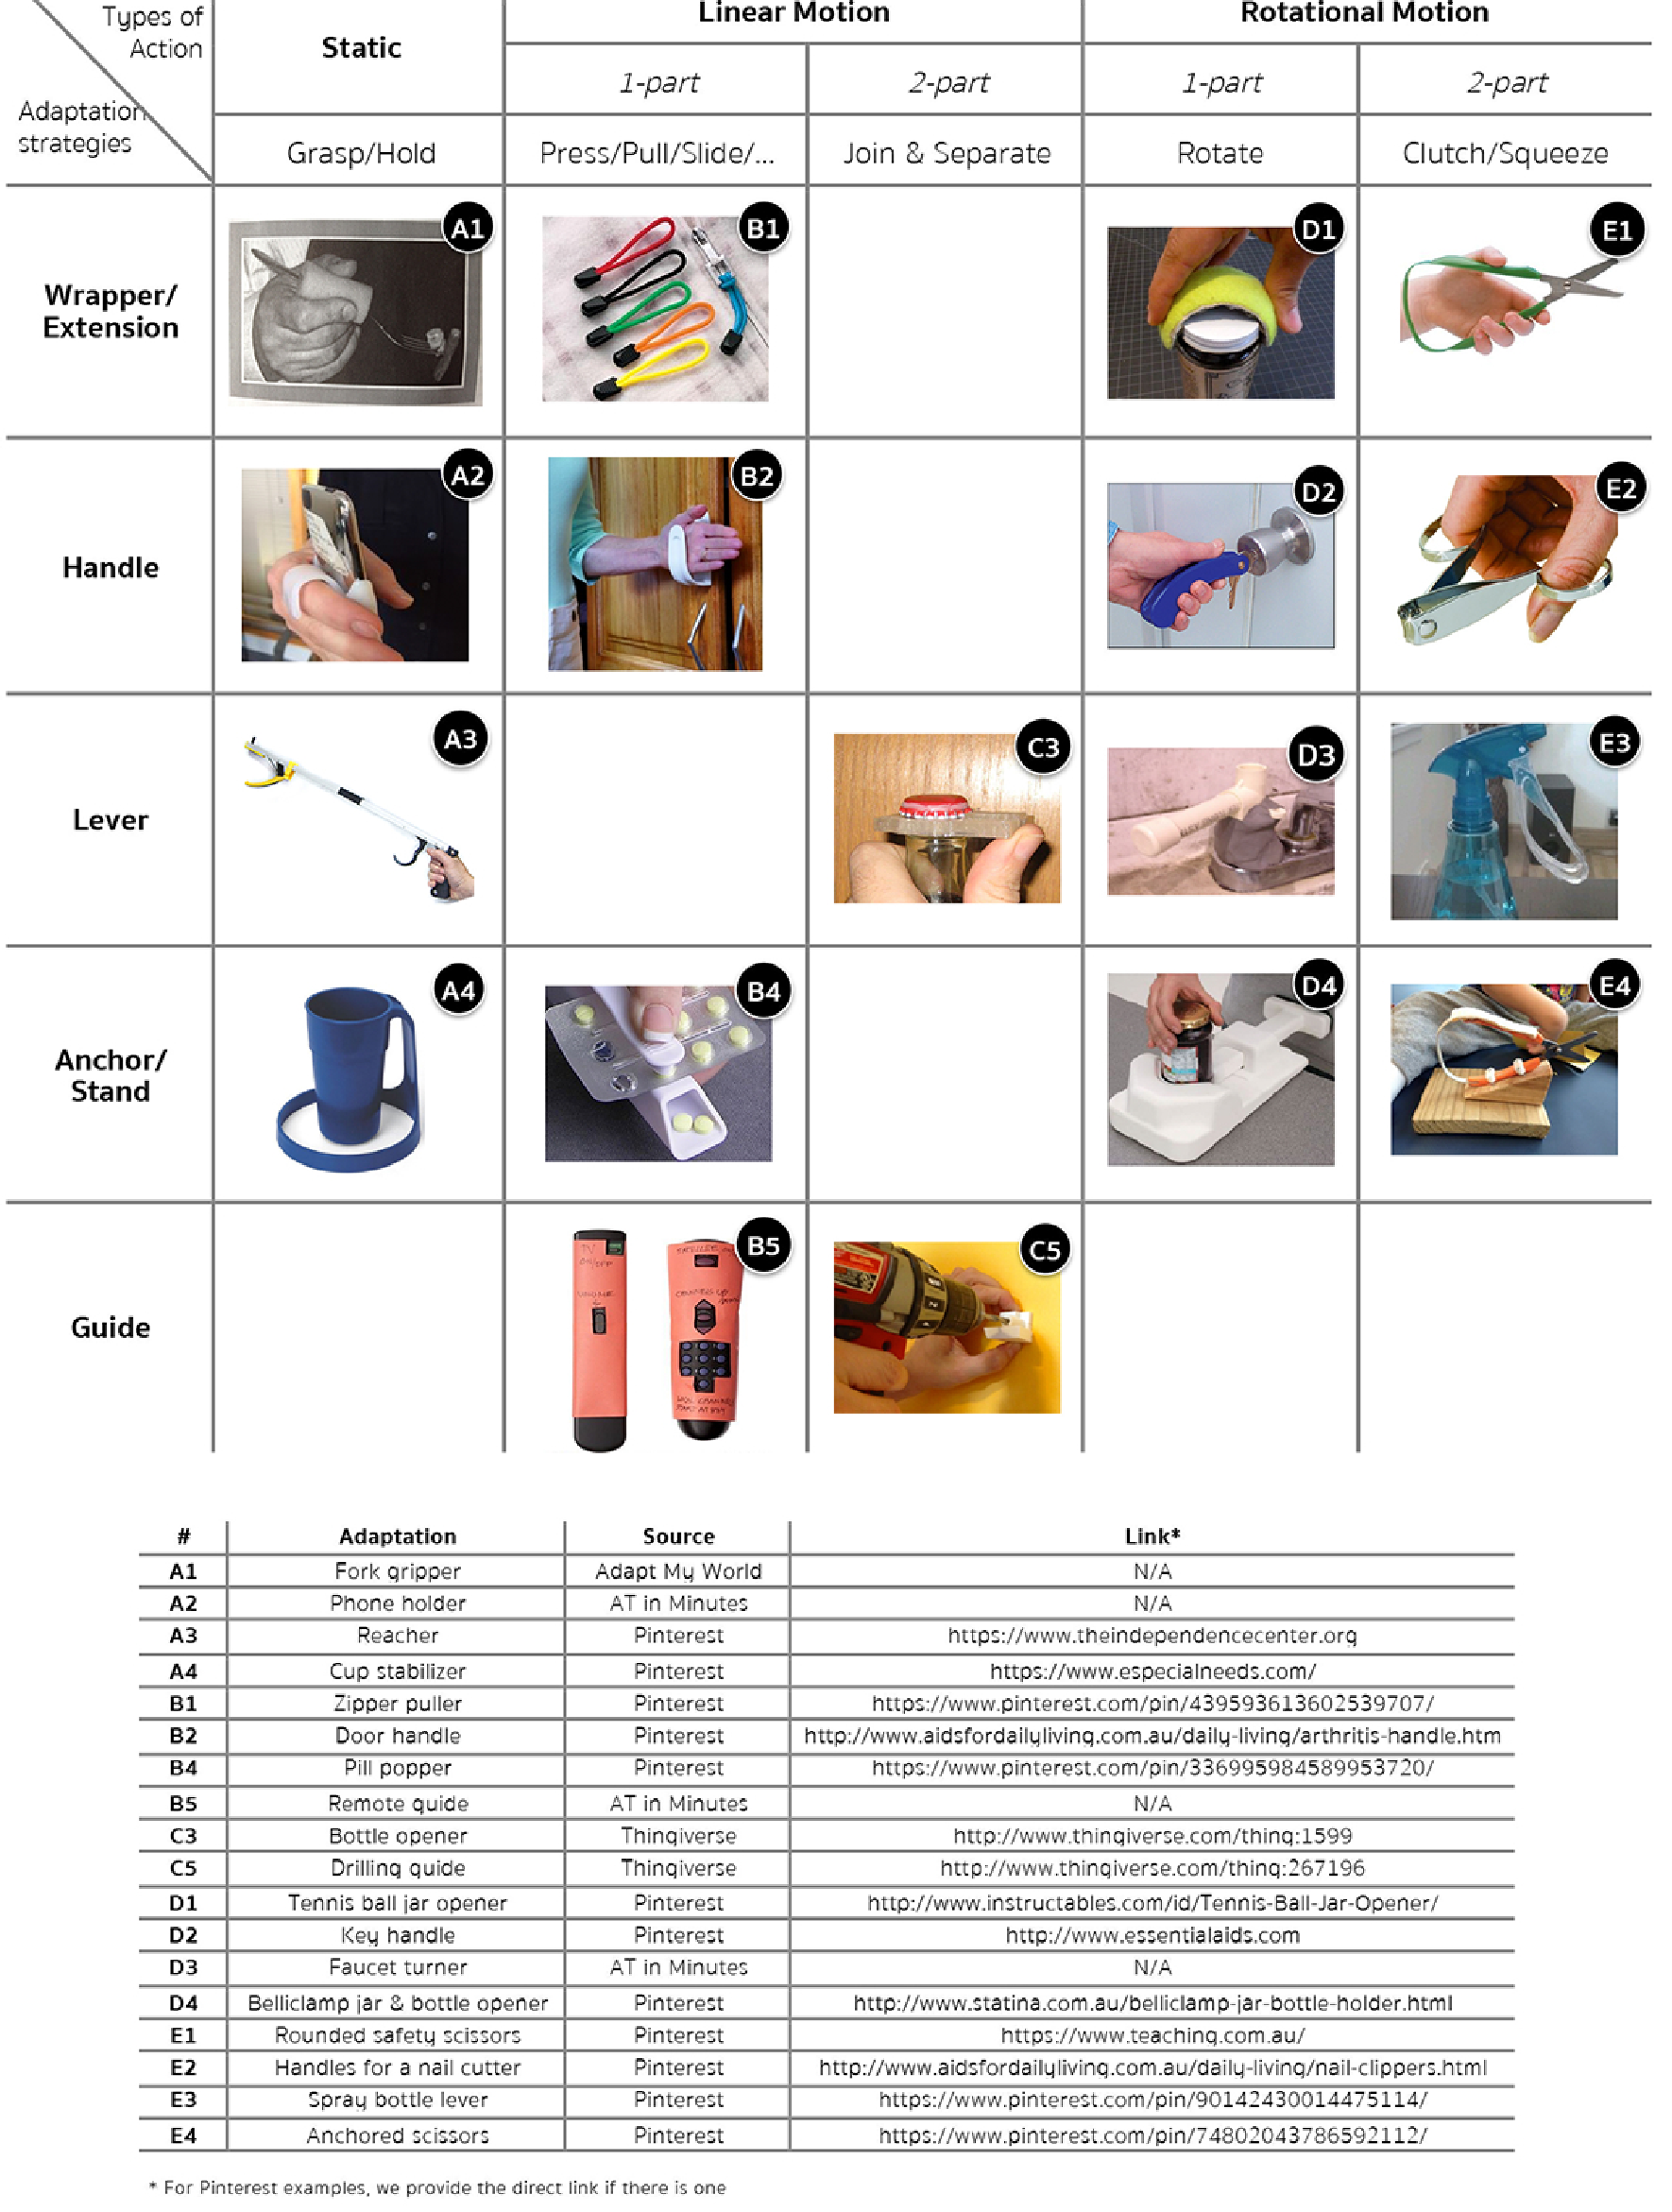
\includegraphics[width=0.9\textwidth]{figures/reprise_adaptation_design_space_v2.pdf}
  \caption{A design space of adaptations summarized from over 3000 existing examples: five major adaptation strategies support various types of actions, from static grasp and hold, to linear and rotational motion that involves one or multiple parts of the objects.}~\label{fig:reprise_design_space}
\end{figure*}

\section{A Design Space of Adaptation Strategies}
For years, well before digital fabrication was widespread, people have been taking a `bricolage' approach for making adaptations on objects that would otherwise be difficult to use. In particular, many innovative solutions came from the need to create assistive technologies (AT) for people with special needs. For example, Werner documented his effort in making assistive technology for village children with very limited resources \cite{werner1987disabled}. Books like \cite{plaxen2005adapt, willkolmm2013assistive, 9781933940021} have compiled simple recipes for individuals to adapt household items and tools with materials that can easily be found at home. Although started with a small and specific audience, these AT design and making solutions usually have a broader impact and implication on universal design \cite{de2011design}. 

Another source of inspiration is online communities such as Thingiverse \cite{thingiverse} and Pinterest \cite{pinterest}, which curate a repertoire of lifehacking solutions people have explored and shared with one another. Recent work by Buehler et al. \cite{buehler2015sharing} has summarized a plethora of assistive technology from Thingiverse, which suggests promising opportunities of learning from these resources.

To inform the computational design of adaptation, we collected and reviewed over 3000 lifehacking and assistive technology examples from the aforementioned literature (85 from \cite{plaxen2005adapt}, 56 from \cite{willkolmm2013assistive}, and 33 from \cite{robitaille2010illustrated}) and online communities (950 from Pinterest  and 2028 from Thingiverse using queries `assistive', `technology' and `adaptation'). Amongst these examples, we identified adaptation designs, and  organized them into themes in a bottom-up fashion. This sampling process continued until we felt that we had reached saturation.

% Rather than attempting to exhaust all possible assistive technology, our goal here was to follow a bottom-up approach: building up a large body of examples, filtering them with a focus on adaptation, and summarizing the findings to inform the design of Reprise.

We present our findings as a design space of adaptation strategies. As shown in Figure~\ref{fig:reprise_design_space}, we identified five major categories of adaptation designs, as well as the types of actions they support to hold, control or operate the objects. While some examples might fit in multiple categories, this design space captures the range of ideas we found in our review and suggests opportunities for novel adaptations (which we discuss in the Results section).

\textbf{\#1 Wrapper/Extension} is something wrapped around an existing object or an extension that lengthens or expands it. Wrapper and extension support various actions with objects. A wrapper can be used to soften the grip (A1), or to assist with grabbing and rotating an object  with less force or less fine motor control (D1). An extension can help with pulling an object (B1) or--with a specific design--to enhance safety for cutting tools (E1).

\textbf{\#2 Handle} is an add-on grippable part attached to an existing object, which makes the object easier to hold (A2), pull (B2), or rotate (D2). Adding handles also helps with clutching, such as using a nail cutter (E2).

\textbf{\#3 Lever} is a structure added to an existing object, usually to make it easier to be turned or rotated, such as the lever used in D3 for turning a faucet, or in E3 for squeezing a spray bottle. In other cases, a lever also affords actions other than rotation, such as grabbing objects (A3), or opening a beer bottle (C3).

\textbf{\#4 Anchor/Stand} is a structure with which an existing object can be stably situated or affixed to the environment. Figure~\ref{fig:reprise_design_space} shows a stand to hold the cup stable (A4), a pill popper for holding a pack of pills and popping them out (B4), a clamp for holding a jar or bottle for easier opening (D4), and an anchor for a pair of scissors for situated use (E4).

\textbf{\#5 Guide} is a structure that guides the movement of, or against, certain objects or their components. B5 shows a guide for locating and pressing buttons on remote controls. C5 is a guide for drilling a screw vertically towards and into a surface. 

Having summarized these five major adaptation strategies, below we describe the technical details of Reprise--a tool that integrates and implements these strategies for generating 3D printable adaptations.

\begin{figure*}
  \centering
  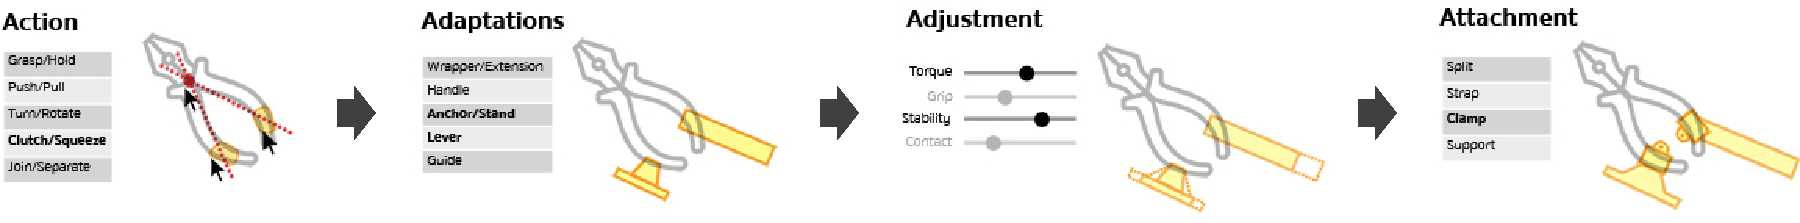
\includegraphics[width=1\textwidth]{figures/reprise_sys_overview_v1.pdf}
  \caption{The design workflow of Reprise. Start with specifying the types of \textit{action} applied on an object, which serves as input for generating user-selected \textit{adaptations}. The initial design can be further customized by \textit{adjusting} a set of parameters. Finally, extra fasteners can be added to make adaptations more \textit{attachable} onto the object.}~\label{fig:reprise_sys_overview}
\end{figure*}

\section{Reprise: Computational Design of Adaptations}
Figure~\ref{fig:reprise_sys_overview} shows the workflow of Reprise. Users start with importing a 3D model of an object they want to adapt, specify what types of action is applied, and on which parts of the object. Next they select an adaptation strategy from a library provided by Reprise, which automatically generates the geometry. This initial design can then be customized by adjusting a set of parameters. Finally, extra fasteners can be added to better attach the adaptations onto the object. Reprise then exports all the generated geometry as 3D printable STL files.

\subsection{Techniques for Specifying Types of Action with an Object}
As a user selects a type of action, Reprise provides interaction techniques for specifying where and how the action is applied on the object. As 3D geometry itself does not encode how an object is used in the real world, Reprise's techniques enable the users to specify this information \textit{in situ}, which later serves as input parameters for generating adaptations. Most of these techniques--as described below--start with the user selecting one ore more \textit{points of action}--the locations on the object where it will be held, controlled, or manipulated.

\textbf{Grasp/Hold} As shown in Figure~\ref{fig:reprise_grasp}, Reprise displays a virtual hand, which can be rotated by moving the mouse cursor around the point of action. This allows users to describe the relative orientation between the grasping hand and the object, such as forming a cylindrical grasp \cite{9780323033848} on a fork (Figure~\ref{fig:reprise_grasp}a), or a spherical grasp \cite{9780323033848} on the cap of a water bottle (Figure~\ref{fig:reprise_grasp}b). Reprise also provides a simple jig (Figure~\ref{fig:reprise_hand_measuring}) for measuring the target user's hand size, which can then be entered into the system.

\begin{figure}[h!]
  \centering
  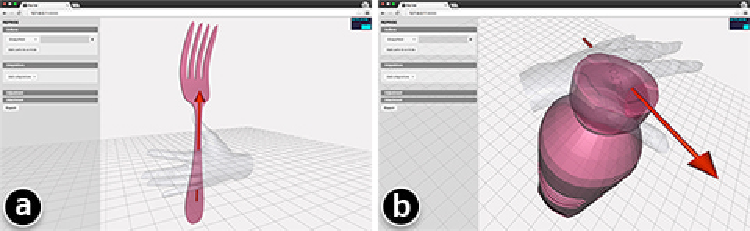
\includegraphics[width=0.75\textwidth]{figures/reprise_grasp_v1.pdf}
\caption{Reprise shows a virtual hand to let the user specify how an object is grasped, such as forming a cylindrical grasp on a knife (a), or a spherical grasp on a bottle (b).}~\label{fig:reprise_grasp}
\end{figure}

\textbf{Push/Pull} A spherical control is used to let the user specify the direction of the push/pull, such as pressing a small power button on a remote (Figure~\ref{fig:reprise_pushpull}a), or pulling a zipper pull horizontally (Figure~\ref{fig:reprise_pushpull}b).

\begin{figure}[h!]
  \centering
  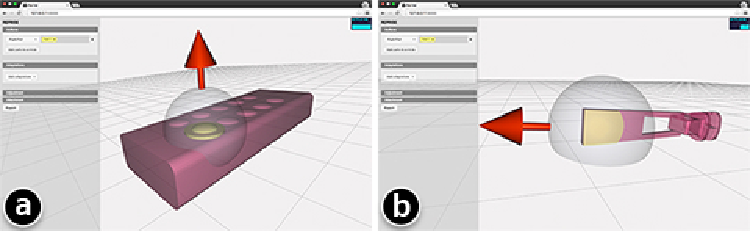
\includegraphics[width=0.75\textwidth]{figures/reprise_pushpull_v1.pdf}
  \caption{Reprise uses a spherical control for specifying pushing/pulling an object, such as pressing a button on a remote control (a), or pulling a zipper (b)}~\label{fig:reprise_pushpull}
\end{figure}

\textbf{Rotate} The user selects the plane ($XY$, $YZ$ or $ZX$) on which the object is rotated, such as the vertical plane on which to turn a door handle (Figure~\ref{fig:reprise_rotate}b). Next the user selects the fulcrum (Figure~\ref{fig:reprise_rotate}c) within that plane. Reprise dynamically displays an arrow pointing from the fulcrum to the point of action to help the user specify the rotating arm (shown as the arrow).
\vskip 5pt

\begin{figure}[h!]
  \centering
  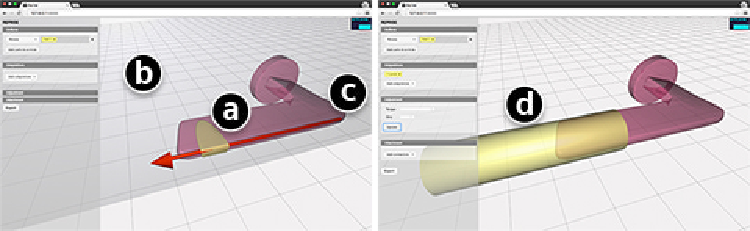
\includegraphics[width=0.75\textwidth]{figures/reprise_rotate_v2.pdf}
  \caption{To specify rotating an object, Reprise lets a user select where the object is held (a), on which plane it is rotated (b), and the fulcrum of rotation (c). The red arrow shows the rotation arm along which a lever can be generated (d).}~\label{fig:reprise_rotate}
\end{figure}

\textbf{Clutch} usually involves two components, such as clutching the two handles of a cutter. Thus the user will select two points of action on the object, such as the handle and the neck of a spray bottle. The plane of clutching is then computed from the normals of the selected points as well as the line segment formed between them. Similar to Rotate, the user then selects a fulcrum on that plane where two arrows are shown indicating the directions of the clutching arms ((Figure~\ref{fig:reprise_clutch}a).

\textbf{Join/Separate} involves two objects moving towards or away from each other. To simplify the problem, Reprise uses their bounding boxes to describe how the objects will be joined or separated. Specifically, the user will select two faces, respectively, from the two bounding boxes, which then shows the direction along which the two objects will moved towards or away from one another. For example, as shown in Figure~\ref{fig:reprise_joinseparate}a, the key would go into the lock hole along its teeth as indicated by the arrows.

\begin{figure}[t]
  \centering
  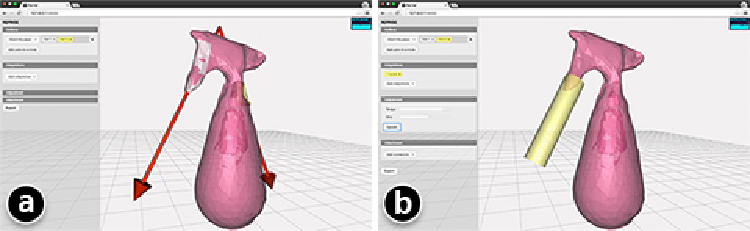
\includegraphics[width=0.75\textwidth]{figures/reprise_clutch_v1.pdf}
  \caption{To specify clutching, the user selects the two parts of the object that are being clutched and then the fulcrum. The red arrows indicate the directions of the clutching arms (a). The user can generate a lever for clutching the spray bottle, while holding its body in hand (b).}~\label{fig:reprise_clutch}
\end{figure}

\begin{figure}[t]
  \centering
  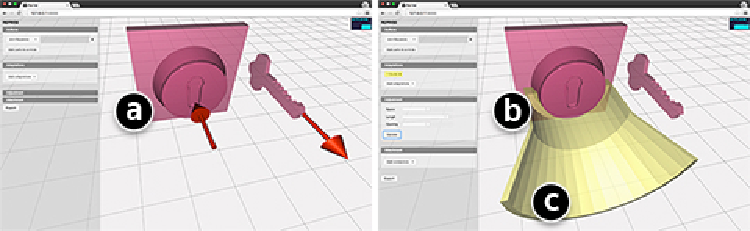
\includegraphics[width=0.75\textwidth]{figures/reprise_joinseparate_v1.pdf}
  \caption{Reprise lets the user specify moving one object towards or away from another, such as putting a key into a lock hole.}~\label{fig:reprise_joinseparate}
\end{figure}

%It is also possible to specify more than one action with an object. For example, for the spray bottle in Figure~\ref{fig:reprise_clutch}, one can also specify a secondary action of `Grasp/Hold' around neck of the bottle.

\subsection{Computationally Generating Adaptations}
Taking the user-specified actions as input parameters, Reprise then provides a list of strategies for rapidly generating the initial design of adaptations. The specific methods for generating these models are based on the aforementioned survey of existing adaptation examples (Figure~\ref{fig:reprise_design_space}). In generating these adaptations, Reprise uses variations of a cylindrical geometry as the primary building blocks, and a series of Constructive Solid Geometry (CSG) operations for creating the specific adaptations. 

\begin{figure}[b]
  \vskip 5pt
  \centering
  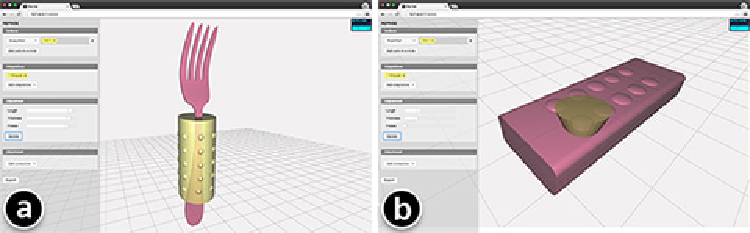
\includegraphics[width=0.75\textwidth]{figures/reprise_wrapper_v1.pdf}
  \caption{Reprise can generate a wrapper--a cylindrical structure bounding part of an object (a), or an extension--an extrusion from a selected area of the object (b).}~\label{fig:reprise_wrapper}
\end{figure}

For example, a cylinder wrapping around part of an object can make a wrapper (Figure~\ref{fig:reprise_wrapper}a) or a lever (Figure~\ref{fig:reprise_rotate}b and Figure~\ref{fig:reprise_clutch}b). Extruding a cylindrical structure from an object's surface creates an extension, such as enlarging a button on a remote control (Figure~\ref{fig:reprise_wrapper}b). To make an anchor, Reprise creates a cylindrical pillar that connects to a rectangular base at the bottom, and to the object at the top (Figure~\ref{fig:reprise_pipeclamp}a). When creating a guide, it is also possible to use an object's bounding cylinder to represent its path of movement, which creates a `tunnel' (Figure~\ref{fig:reprise_joinseparate}b) with a wide `opening' at the entrance (Figure~\ref{fig:reprise_joinseparate}c). By default Reprise displays the models in 1:1 scale to let the user get a concrete sense of the adaptations' size and dimensions when adjusting these parameters.

\subsection{Adjusting Design Parameters for Customization}
With the initial design of the adaptations, Reprise provides users with simple slider controls to adjust the design parameters for further customization. For example, for gripping, they can lengthen a wrapper so that it can be held by multiple fingers (the sizes of which can be measured using a tool described later in Figure~\ref{fig:reprise_hand_measuring}); they can also adjust the radii of the cylindrical components, or add small bumps on the surface to tighten the grip (Figure~\ref{fig:reprise_wrapper}a). To enhance strength and support, they can increase the torque of the levers, or give the anchor or stand a larger base. For easier hand coordination, they can widen the opening in a guide, making it easier to move one object into the `tunnel' and towards the other object (Figure~\ref{fig:reprise_joinseparate}c). To adjust the overall size, they can make a handle more elliptic or vary the length of its arc (Figure~\ref{fig:reprise_all_designs}c).

To help users navigate the rich parameter space, Reprise also allows them, with one click, to generate a large set of design variations (Figure~\ref{fig:reprise_all_designs}a$\rightarrow$b), similar to the technique in Side Views \cite{terry2002side}. This provides them with a more intuitive way of browsing and comparing different designs, select one that best matches what they have in mind (Figure~\ref{fig:reprise_all_designs}b$\rightarrow$c), and from which they can continue to customize the model (Figure~\ref{fig:reprise_all_designs}c). For example, as shown in Figure~\ref{fig:reprise_all_designs}, to make an adaptation for grasping a fork, the user can select wrappers of different length, thickness, and tightness, as well as handles of different sizes and styles.

\begin{figure}[h!]
  \vskip 5pt
  \centering
  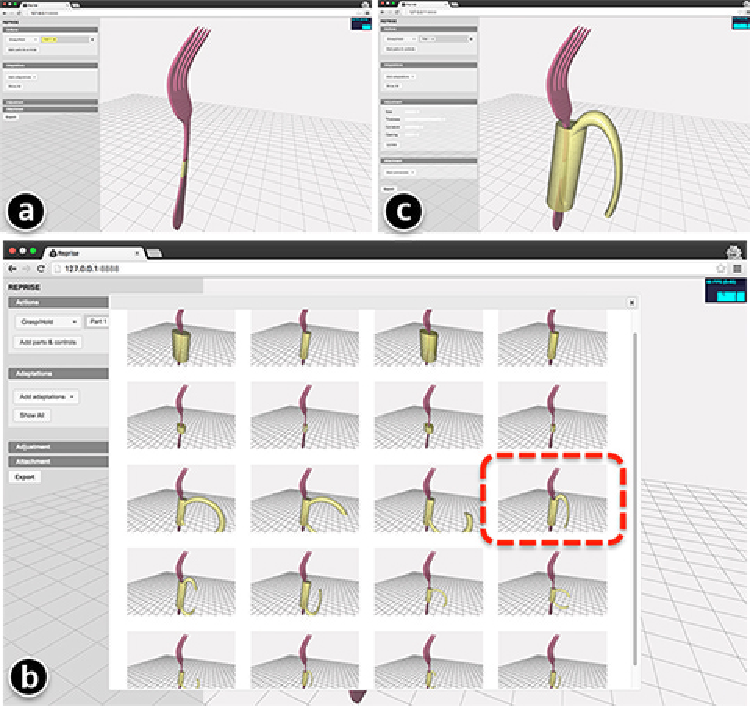
\includegraphics[width=0.75\textwidth]{figures/reprise_all_designs_v2.pdf}
  \caption{Besides using sliders, users can also click a button to generate a large set of design variations (ab), from which they can select one that best matches the design they have in mind, and continue to develop it from that model (c).}~\label{fig:reprise_all_designs}
\end{figure}

\subsection{Attaching Adaptations onto Real World Objects}
As a last step, the user normally wants to generate some attaching mechanism(s) for installing the adaptations onto the object. Prior work, such as Encore \cite{chen2015encore} and AutoConnect \cite{koyama2015autoconnect}, has explored a range of attachment techniques, which can be used as a post-processing step to install the adaptations. 

In addition, Reprise also offers several simple built-in techniques for making the adaptation more attachable. For example, `Split' lets the user draw a stroke on the model of the adaptation (Figure~\ref{fig:reprise_split}a) to split it into halves (Figure~\ref{fig:reprise_split}b), such as splitting a wrapper so that a fork can be placed in it (Figure~\ref{fig:reprise_wrapper_results}a). `Clamp' lets users create a simple pipe clamp: first positioning the pipe (Figure~\ref{fig:reprise_pipeclamp}b) and then stroking a line to cut the pipe open and generate clamps (Figure~\ref{fig:reprise_pipeclamp}cd) where a bolt can be used to fasten the structure. `Beams' can be added to the adaptation by selecting a point on the object and another point on the adaptation (Figure~\ref{fig:reprise_beams}ab). This will generate structures to further support the object, such as to further stabilize a mug (Figure~\ref{fig:reprise_beams}c).
\vskip 3pt

% `Strap' is implemented from Encore \cite{chen2015encore}: the user also draws around part of the object, which creates space in the adaptation for a strap to go through and wrap around the object.

\begin{figure}[h!]
  \vskip 10pt
  \centering
  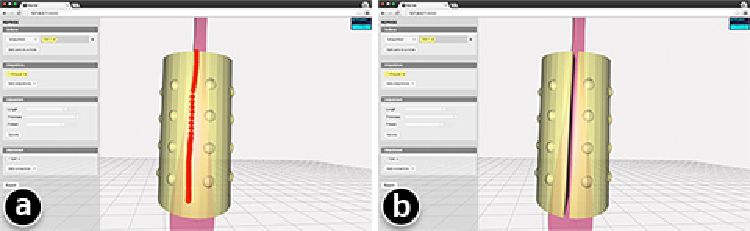
\includegraphics[width=0.75\textwidth]{figures/reprise_split_v1.pdf}
  \caption{Reprise provides a simple technique to split an adaptation in halves so an object, such as this fork, can be put inside a wrapper (Figure~\ref{fig:reprise_wrapper_results}a).}~\label{fig:reprise_split}
\end{figure}

\begin{figure}[h!]
  \vskip 8pt
  \centering
  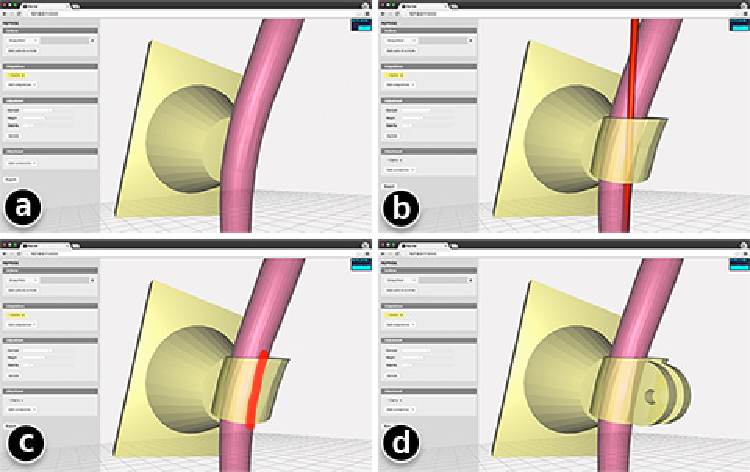
\includegraphics[width=0.75\textwidth]{figures/reprise_pipeclamp_v1.pdf}
  \caption{A pipe clamp, provided by Reprise, attaches the generated stand (a) to the object. Clicking on the object places the pipe (b). Another stroke cuts it open and adds a pair of clamps (cd).}~\label{fig:reprise_pipeclamp}
\end{figure}

\begin{figure}[h!]
  \vskip 8pt
  \centering
  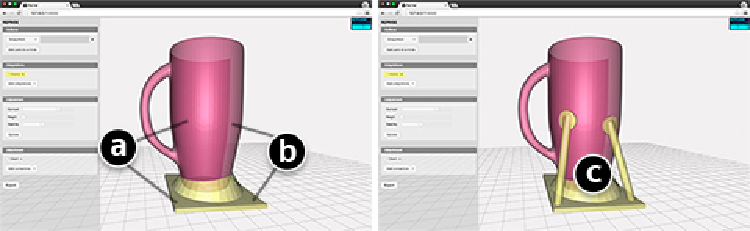
\includegraphics[width=0.75\textwidth]{figures/reprise_beams_v1.pdf}
  \caption{Beams can further support the object for an adaptation. To generate one, simply select a point on the object and another point on the adaptation.}~\label{fig:reprise_beams}
\end{figure}

In some cases, part of an object is not accessible or should not be occluded by the adaptations, such as a phone's screen. Reprise allows a user to specify which part of the object should be excluded when generating adaptations. As shown in Figure~\ref{fig:reprise_inaccessible}a, the phone's screen is marked as inaccessible (red), and accordingly the generated handle avoids covering the screen area (Figure~\ref{fig:reprise_inaccessible}b).

\begin{figure}[h!]
  \vskip 7pt
	\centering
	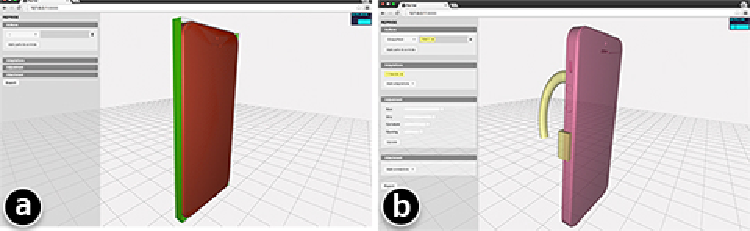
\includegraphics[width=0.75\textwidth]{figures/reprise_inaccessible_v1.pdf}
	\caption{As the phone's screen is marked as inaccessible (red) by an adaptation, the generated handle avoids covering that area.}~\label{fig:reprise_inaccessible}
\end{figure}

\subsection{Implementation, Measurement and Fabrication}
Reprise was implemented using JavaScript with three.js\footnote{\url{http://threejs.org/}} and OpenJSCAD\footnote{\url{http://openjscad.org/}}. The tool can run readily inside a modern browser. Reprise curates a 3D model repository of common household items and hand tools; alternatively, it also uses Skanect\footnote{\url{http://skanect.occipital.com/}} and the Makerbot Digitizer \footnote{\url{http://store.makerbot.com/digitizer}} for digitalizing objects. The spray bottle in Figure~\ref{fig:reprise_clutch} was scanned using the Skanect system.

For some adaptations, users might need to measure the hand or finger sizes of the person. Reprise comes with a simple measuring tool (Figure~\ref{fig:reprise_hand_measuring}) that can be printed (and cut) on a piece of paper, or made with a laser cutter. The hand measuring part is based on a method for determining the size for a golf glove\footnote{\url{http://www.jumbomax.com/sizing/}}. The finger part is based-on standard ring-size metrics.

\begin{figure}[h!]
\vskip 7pt
  \centering
  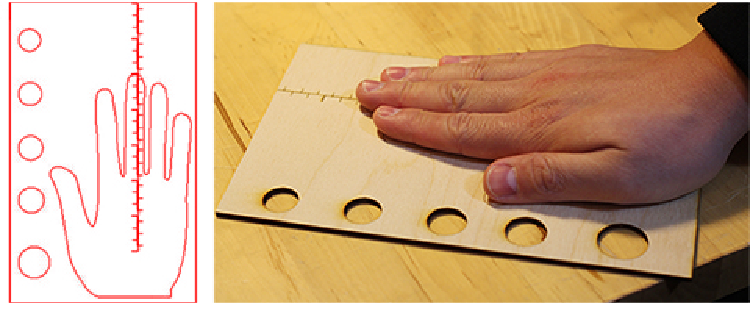
\includegraphics[width=0.9\textwidth]{figures/reprise_hand_measuring_v1.pdf}
\caption{Reprise also provides an SVG file for making a measuring tool for adaptations that require fitting users' hand or fingers. This one shown above was laser cut.}~\label{fig:reprise_hand_measuring}
\end{figure}

For fabrication, we used material with various softness, ranging from regular PLA, to SemiFlex\footnote{\url{http://www.ninjaflex3d.com/products/semiflex/}}, Nylon-based\footnote{\url{http://www.graphene3dlab.com/}} or NinjaFlex\footnote{\url{http://www.ninjaflex3d.com/products/ninjaflex-filaments/}}. All the results--as we demonstrate below--were fabricated using an inexpensive Printrbot Play 3D printer\footnote{\url{https://printrbot.com/shop/assembled-printrbot-play/}}.

%\hl{Currently Reprise only deals with geometry; in the future it would be interesting to incorporate some consideration of material, such as recommending what filament to use for a given kind of adaptation.} 

\section{Results and Validation Through Replication}
Compared to traditional CAD tools where models are mostly created from scratch, Reprise has integrated application domain specific knowledge that allows users to specify, generate and customize adaptations at a higher level. While there may remain some usability issues with our tool, this application domain targeted approach clearly allows adaptations to be specified much more easily than trying to create them as unstructured arbitrary geometry in a general-purpose tool.  However, this ease of use can come at a price, and this raises the important issue of whether the tool can create a wide range of objects to cover an interesting and useful space. To answer this more difficult question, we validate Reprise by focusing on its breadth of expressiveness.  In particular, we used it to replicate a wide spread of existing adaptation examples. This demonstrates the potential for Reprise to support the full range of adaptations that are demonstrably useful in the real world.

% We chose to perform this exercise as an expert user, to overcome the limit of a laboratory study where each participant only has a limited time to explore or iterate a few different adaptation designs.

Specifically, we chose to replicate representative cases from different `cells' in the design space of adaptations (Figure~\ref{fig:reprise_design_space}). Below we showcase our results, discuss issues that arose during the process, and identify cases where Reprise is not yet able to generate the adaptations, which suggest opportunities for future work.

% Due to the time-consuming and iterative nature of 3D printing, the time frame of a typical usability study would limit the number of adaptations that can be designed and fabricated. As such, we chose to

\textbf{\#1 Wrappers/Extensions}
As shown in Figure~\ref{fig:reprise_wrapper_results}, Reprise was able to replicate all the four wrapper/extension examples in the design space. The virtual hand was effective in positioning the wrapper at the right place on the objects. However, in the case of the cutter handle, we found that the simple cylindrical structures did not fully conform to the curvature of the handles (Figure~\ref{fig:reprise_wrapper_results}d). A new feature for future work would be to `curve' the wrapper so that it can better represent the original geometry of the object.

% As shown in Figure~\ref{fig:reprise_wrapper_results}, Reprise replicated the gripper for a fork (Figure~\ref{fig:reprise_wrapper_results}a), the extension for a zipper pull (Figure~\ref{fig:reprise_wrapper_results}b), and the tennis ball opener (Figure~\ref{fig:reprise_wrapper_results}c), all of which we fabricated  using either Nylon-based or Ninja Flex soft material. The cutter handle wrapper (Figure~\ref{fig:reprise_wrapper_results}d) supports clutching and thus meets the Figure~\ref{fig:reprise_design_space}-E1 category; however its purpose is different from the existing example (Figure~\ref{fig:reprise_wrapper_results}d inset), which is specifically designed for safety concerns.

\begin{figure}[h!]
  \centering
  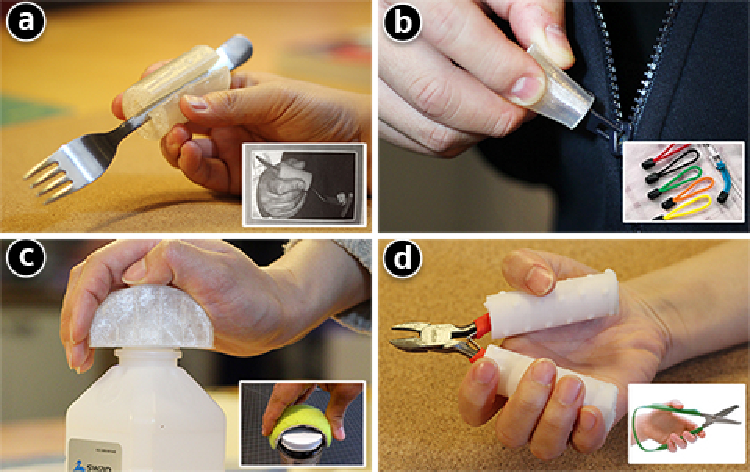
\includegraphics[width=0.75\textwidth]{figures/reprise_wrapper_results_v1.pdf}
  \caption{Replicated wrapper/extension examples. Ninjaflex was used for the fork wrapper (a), zipper handle extension (b), and the bottle lid wrapper (c). Nylon-based soft material was used for the cutter. }~\label{fig:reprise_wrapper_results}
\end{figure}


\textbf{\#2 Handles}
All types of handle examples in the design space were replicated using Reprise (Figure~\ref{fig:reprise_handle_results}). Reprise allows users to explore different handle designs, such as making a `closed loop' for holding and turning a key (Figure~\ref{fig:reprise_handle_results}c), or half-open for easier placement of the hand when holding a phone (Figure~\ref{fig:reprise_handle_results}a) or pulling open a cabinet door (Figure~\ref{fig:reprise_handle_results}b). 

A single handle can be used to stabilize the grip of a pen (Figure~\ref{fig:reprise_combine_adaptations}a) while it is also possible to combine multiple handles to match different fingers (Figure~\ref{fig:reprise_handle_results}d). In particular, for fingers, initially we found it really hard to specify a fixed spatial relationship between them and the handles, as their position and orientation could vary from time to time while holding an object. Later we found that using soft material could mitigate this problem, as its deformable nature offers a range of adjustable configurations. Although Reprise operates at the geometry level, it is possible, as a future step, to fine tune the geometry of a handle as a way to `program' its range of configuration when printed with soft material.
\vskip 5pt
% All types of handle examples in the design space were replicated using Reprise (Figure~\ref{fig:reprise_handle_results}). Reprise allows users to explore different handle designs, such as making a `closed loop' for holding and turning a key (Figure~\ref{fig:reprise_handle_results}c), or half-open for easier placement of the hand when holding a phone (Figure~\ref{fig:reprise_handle_results}a) or pulling open a cabinet door (Figure~\ref{fig:reprise_handle_results}b). Multiple handles can also be combined to match with different fingers (Figure~\ref{fig:reprise_handle_results}d).

%\vskip 2pt

\begin{figure}[h!]
  \centering
  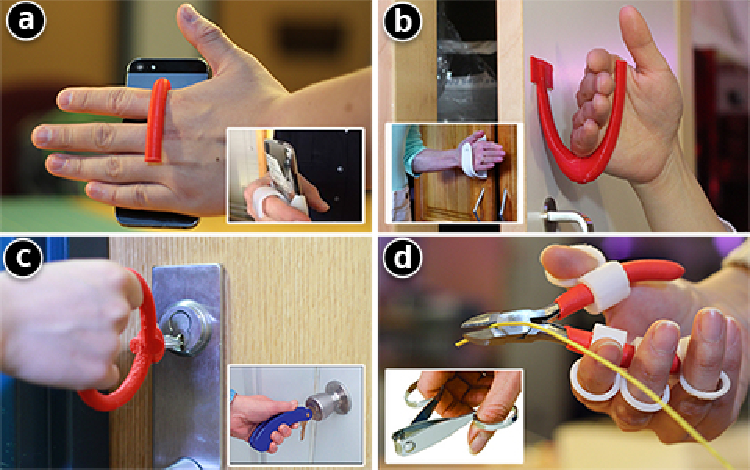
\includegraphics[width=0.75\textwidth]{figures/reprise_handle_results_v1.pdf}
  \caption{Replicated handle examples.}~\label{fig:reprise_handle_results}
\end{figure}

\textbf{\#3 Levers}
Figure~\ref{fig:reprise_lever_results} shows Reprise' replication of levers. One current limitation we found is that Reprise can only generate levers where part of the existing object has a degree of freedom to be rotated or squeezed. In the future we plan to explore other use cases of a lever, such as for clamping (Figure~\ref{fig:reprise_design_space}-A3) or separating (Figure~\ref{fig:reprise_design_space}-C3) static objects.
\vskip 3pt

% For rotation, we created a lever for a small cylindrical light switch (Figure~\ref{fig:reprise_lever_results}a), in spirit similar to the faucet design in Figure~\ref{fig:reprise_design_space}-D3. We also adapted a spray bottle to replicate the existing example (Figure~\ref{fig:reprise_lever_results}b). Currently Reprise can only generate levers where part of the existing object has a degree of freedom to be rotated or clutched. In the future we plan to explore other use cases of a lever, such as for clamping (Figure~\ref{fig:reprise_design_space}-A3) or separating (Figure~\ref{fig:reprise_design_space}-C3) static objects. 

\begin{figure}[h!]
\vskip 5pt
  \centering
  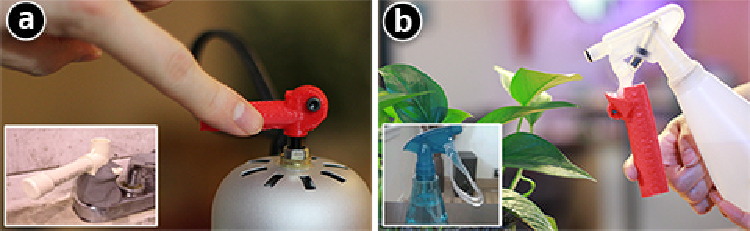
\includegraphics[width=0.75\textwidth]{figures/reprise_lever_results_v1.pdf}
  \caption{Replicated lever examples.}~\label{fig:reprise_lever_results}
\end{figure}

\textbf{\#4 Anchors/Stands}
Besides the aforementioned cutter, we also replicated two other anchor/stand examples as shown in Figure~\ref{fig:reprise_anchor_results}. When making these examples, we often found it necessary to add extra fasteners or support structures, such as the pipe clamp for the cutter (Figure~\ref{fig:reprise_anchor_results}a) and the supporting beams for the mug and the sharpie anchor (Figure~\ref{fig:reprise_anchor_results}bc). Rather than adding them as a follow-up step, future work could integrate these components parametrically as part of the generated adaptation.

% Besides the aforementioned cutter, we also replicated the stabilized cup design (Figure~\ref{fig:reprise_anchor_results}b) and an anchor for holding a sharpie (which is in spirit similar to the Belliclamp device in Figure~\ref{fig:reprise_design_space}-D4). Both our sharpie anchor and the Belliclamp also involve multiple actions--joining/separating objects by means of pushing, pulling or rotation.

\begin{figure}[t]
  \centering
  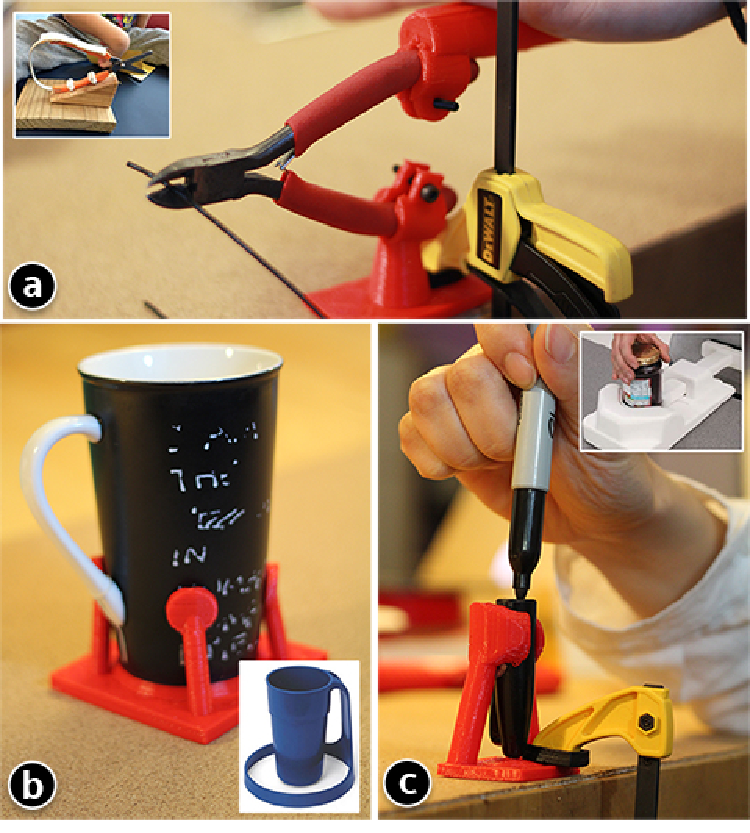
\includegraphics[width=0.7\textwidth]{figures/reprise_anchor_results_v1.pdf}
  \caption{Replicated anchor/stand examples.}~\label{fig:reprise_anchor_results}
\end{figure}

\textbf{\#5 Guides}
Inspired by the drilling guide example (Figure~\ref{fig:reprise_design_space}-C5), we used Reprise to generate similar structures for guiding a key towards a lock (Figure~\ref{fig:reprise_guide_results}a) and putting a sharpie back into its cap (Figure~\ref{fig:reprise_guide_results}b). We did not replicate the remote control example as it stands (Figure~\ref{fig:reprise_design_space}-B5), as it seems simple enough to be made with paper, and further it sacrificially occludes other buttons. Instead, we opted for an alternate design--an extension on the button that makes it a larger target for pressing (Figure~\ref{fig:reprise_wrapper}b). It is interesting to see that in this case an extension can also serve as a guide, which suggests the possibility of `remixing' categorically different adaptation strategies.


% Inspired by the drilling guide example (Figure~\ref{fig:reprise_design_space}-C5), we used Reprise to generate similar structures for guiding a key towards the lock (Figure~\ref{fig:reprise_guide_results}a) and putting a sharpie back into its cap (Figure~\ref{fig:reprise_guide_results}b). We did not replicate the remote control example (Figure~\ref{fig:reprise_design_space}-B5), as there seems to be an easier solution--cutting and pasting pieces of paper\footnote{However, to avoid occluding other buttons, Reprise can generate an alternate design--an extension on the button that makes it a larger target for pressing (Figure~\ref{fig:reprise_wrapper}b)}. Reprise currently only guides linear motion; in the future it should be possible to explore how to generate guides for other types of motion, such as a guide for turning faucets to get (only) mildly warm water.

\begin{figure}[h!]
  \vskip 5pt
  \centering
  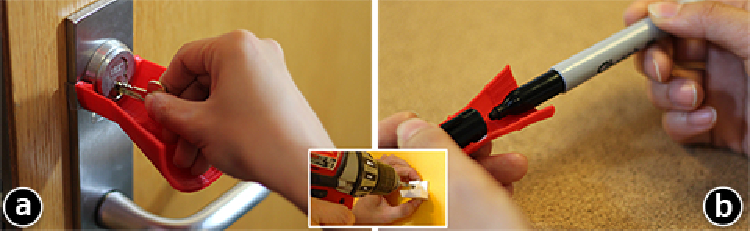
\includegraphics[width=0.75\textwidth]{figures/reprise_guide_results_v1.pdf}
  \caption{Replicated guide examples.}~\label{fig:reprise_guide_results}
\end{figure}

One limitation we found is that Reprise currently only guides linear motion; in the future it should be possible to explore how to generate guides for other types of motion, such as a guide for turning faucets to get (only) mildly warm water.


\section{Discussion and Summary of Designing Adaptations}
Based on our exploration of the design space, tool integration and fabricated results of adaptations, we now discuss existing issues, limitations and potential future work.

\textbf{Combining different adaptations}
With Reprise, it is also possible to combine different adaptation strategies. Figure~\ref{fig:reprise_combine_adaptations} shows a series of sharpie adaptations generated by Reprise, ranging from a handle for holding (Figure~\ref{fig:reprise_combine_adaptations}a), the aforementioned guide (Figure~\ref{fig:reprise_combine_adaptations}b) and anchor (Figure~\ref{fig:reprise_combine_adaptations}c), and finally, a combination of the three (Figure~\ref{fig:reprise_combine_adaptations}d). Our current approach is to incrementally add new adaptation with the previous ones considered as part of the object. However, the ordering of addition could cause adaptations to conflict with one another. For example, adding a handle might make the sharpie no longer fit in the guide installed earlier. Future work could optimize the order of adding multiple adaptations to reduce conflict, or updating existing adaptations as new ones are added.

\begin{figure}[h!]
  \centering
  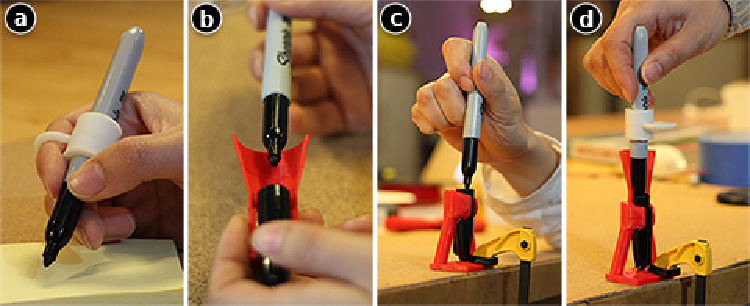
\includegraphics[width=1\textwidth]{figures/reprise_combine_adaptations_v1.pdf}
  \caption{Combining multiple adaptations: a handle (a), a guide (b) and an anchor (c) can be combined into one (super) adaptation (d).}~\label{fig:reprise_combine_adaptations}
\end{figure}


\textbf{Expanding the feedback loop for customization}
Rather than just taking the original object as input, future work could enable a more iterative approach where a printed piece of adaptation can be fed into the system to let the user further customize it. Prior work, such as ModelCraft \cite{song2006modelcraft} could potentially be extended here to let the user annotate printed results for the next design iteration.

\textbf{Scaling up reprise to adapt larger objects}
Most of the objects Reprise adapted so far are hand-sized items or tools. In future it would be interesting to explore larger scaled adaptations, such as making a bath tub safer to walk in/out, or making room entrances or stairwells more accessible. The challenges are two-fold: how to scale up the current design workflow to incorporate large objects, and how to go beyond the usual volume of 3D printers to fabricate the adaptations.

% \textbf{Evaluating the Usability and Learnability of Reprise}
% We designed Reprise with a goal in mind to make the process as simple as possible. Indeed, Reprise dispenses with low-level mesh manipulation--users specify types of actions, generate adaptation models, adjust the design parameters and add attachment aids, all in a few mouse clicks and drags. However, despite the intentional simplicity, Reprise still presents itself as a 3D modeling tool wherein each step does require certain level of understanding in 3D geometry. Future work could test Reprise with users who have little or no 3D modeling experience to reveal whether and where they have difficulty with the design workflow.

\textbf{Combining hand-making and digital fabrication}
Although we designed Reprise for 3D printing, we believe it may work best as a tool that complements existing hand-making approachs, rather than replacing them. Hand-making can capture users' intuition and creativity (even though the outcome is still limited by the materials available and the users' making skill). Future work could transform Reprise's workflow to incorporate or augment handmade prototypes, such as using 3D printed fasteners to connect handmade parts, or to serve as components that require higher functional precision.

\textbf{Using vision-based sensors to capture object usage}
As we designed the virtual hand for specifying different ways of grasping, we realized the possibility of an alternate approach where the person can use an RGB+depth camera (e.g., Kinect) to show their grip by performing it. This seems a more natural way to express one's difficulty with objects. Further, the person's hand shape might also be captured by first gripping a piece of clay \cite{buehler2014coming} and then digitalizing it. Although compelling, this type of vision-based approach has inherent issues, such as the imprecision of the sensors and the general difficulty in reconstructing the captured data into high-fidelity 3D models.

% \textbf{Exploring Mechanism as a New Adaptation Strategy}
% Mechanism provides a simple mechanical system for applying motion to certain objects, usually by replacing the original motion with new type of motion favorable by the users. Figure XXa shows a design sketch of a cam mechanism applied on a spray bottle so that users with difficulty squeezing can instead turning a crank to press the spraying handle. Figure XXb shows a universal joint attached to a screw driver, which accommodates a wider range of angle and hand posture when applying the rotation motion. Figure XXc is simple clutch mechanism as an alternate way of holding an object tight.

%\xac{
%
%* adaptations that handle a range of objects rather than a specific object
%
%* human creativity + machine intelligence/precision
%
%* combining 3d printing and material that is readily available
%
%  adapting large scale objects?
% 
% large scale: https://www.youtube.com/watch?v=CKl_3mnj3dM
%}
%
%\xac{
%* tying shoelaces
%
%* clothes buttons
%}


In my work thus far, either extending or adapting existing objects allows for incremental `delta' for transforming the real world, as their functionality is somewhat dependent on the objects they are attached to. For a non-incremental approach, where brand-new objects are created from scratch, the objects we create will often end up physically interacting with others. A bookshelf will be used to put on books. A chair will be sit on. A step stool will stood upon. How can facilitate the design process so that objects like these can function properly and reliably with real world objects they will be used with. My next chapter proposes a design tool to support users in conducting such fuctionally aware design tasks.
\chapter{User-Driven Structure Design to Support Real World Objects}

\begin{figure} [h]
   \centering
   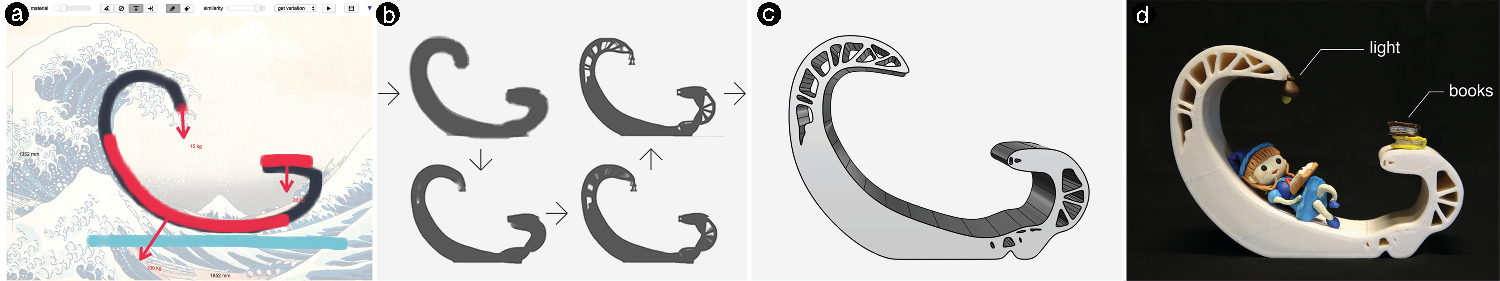
\includegraphics[width=1\textwidth]{figures/kanagawa}
   \caption{Forte is a 2D design tool that takes a user-driven approach of generative design: a user sketches a reading chair inspired by the  painting `The Great Wave off Kanagawa' (a) with specified loading scenario (red arrow forces, blue ground); Forte then generates structures (with real-time feedback) to support the loads while resembling the user's sketch (b), which can then be post-processed to create a 3D fabrication-ready model (cd).}~\label{fig:fig1}
\end{figure}

In both of the previous projects---Encore and Reprise, the design task is based on an existing object and the outcome is some sort of extension that enhances a specific function of that object. While this approach works for creating something incremental (e.g., adaptation), it becomes problematic when scaling up---creating self-contained objects such as bookshelf, step stool, or wine rack.

There are several challenges in designing this class of objects. Foremost, as they are no longer incremental add-ons to existing objects, it would be difficult to create a design \textit{in situ} from these real world objects. Consider making a bookshelf for example. It is less straightforward if one has to start the design with some books; rather, a more intuitive approach is the reverse: create the bookshelf first, then see if it has enough space, or is strong enough to accommodate the books. However, for non-expert users, it is hard to create a functional design by intuition. A user might have an intuition about what their bookshelf should look like, and might be able to sketch the design; but they would probably have trouble making sure that this design would work---that is, supporting all the books to be put on it.

To ensure that a design meets such functional requirement, generative design methods such as \textit{topology optimization}
% \footnote{While `generative design' refers to a broader set of approaches, we focus on the one using topology optimization. The remainders of the paper will use these two terms interchangeably.} 
will automatically optimize material distribution given the constraints of space, material amount and other functional requirements \cite{sigmund200199}.
% =======
% Traditionally, to solve such problems, methods such as topology optimization will automatically optimize material distribution given the constraints of space, material amount and other functional requirements \cite{sigmund200199}.
% >>>>>>> 994990b10e609aa6dd81e7dd787c074591ca4222
Though promising, such methods provide very few ways for users to directly express or manipulate their designs; instead, users have to map their design ideas--often unintuitively--to mathematical input parameters. Further, it is often assumed that a CAD model has been designed prior to using such methods. As a result, there is a lack of support for users' ideation process, and they have little direct control of the optimization's outcome \cite{zhou2016direct}, or ways to effectively iterate their designs.

To address this problem, prior work and existing tools have been focusing on interactively specifying the input parameters \cite{aage2013interactive, Stressto43:online}, adding template-based textures to the optimized results \cite{martinez2015structure}, or contextualizing them with CAD \cite{shea2003towards} or freeform sketching \cite{kazi2017dreamsketch}. However, none of this work lets users directly control how a design should be generated and optimized.

%  \cite{aage2013interactive} and a few existing tools \cite{Stressto43:online} have sought to enable users to spatially manipulate the input parameters, which updates the optimization accordingly; however, this still gives users only indirect control over the results.
% % one approach is to let users provide a 3D model and optimize it while keeping it similar to the original shape \cite{zhou2016direct}. This, however, assumes users already have a fully designed object in mind. 
% Another solution is to directly specify the appearance of the optimized structure by providing examplar visual patterns \cite{martinez2015structure}, which, however, only focuses on low-level textures rather than high-level look-and-feel. To give users more freedom of control, a third approach is to create fabricatable objects via sketching \cite{igarashi2007teddy}; however, often users are not sketching the parts to be optimized \cite{kazi2017dreamsketch}, or when they do there is little direct guidance on improving the sketch for better performance \cite{saul2011sketchchair}. 

% sketch chair
% martinez
% zhou
% !!! stress relief

%Technical Solution
To help address these issues, we present Forte, a sketch-based 2D design tool that takes a user-driven approach for people to directly express and iterate on their ideas through generative design with real-time visual feedback.
%Contribution
Our main contribution is a technical approach that supports a high-level dialog allowing a simpler expression of users' design intent, resulting in a combination of structural performance and less quantifiable objectives to be achieved in the results. Figure~\ref{fig:fig1} shows an exemplar workflow: sketching a reading chair inspired by the famous painting `The Great Wave off Kanagawa'\footnote{\url{https://en.wikipedia.org/wiki/The_Great_Wave_off_Kanagawa}} with a specified loading scenario; Forte then generates structures to support the loads while resembling the user's sketch, which can then be post-processed using external tools (e.g., Rhinoceros) to create a 3D fabrication-ready model.

Specifically, with Forte, users can ask the system to add structures to the original sketch, provide a variation with better performance, or generate optimized internal structures.
Users can globally adjust a `similarity' slider, which controls how much the system will `deviate' from their initial input; they can also locally edit the design by adding or erasing parts of the sketch, which then interactively prompts the system to update based on this new information.
 % while informed of the performance trade-off by a visualization.
Meanwhile, a visualization informs users of the performance trade-off as they iterate on the design.
Building on a fast topology optimization engine \cite{andreassen2011efficient}, Forte enables rapid iteration and exploration, unlike most existing practices that run the process in a non-interactive, batch fashion (even for 2D designs).

\begin{figure*} [t]
  \centering
  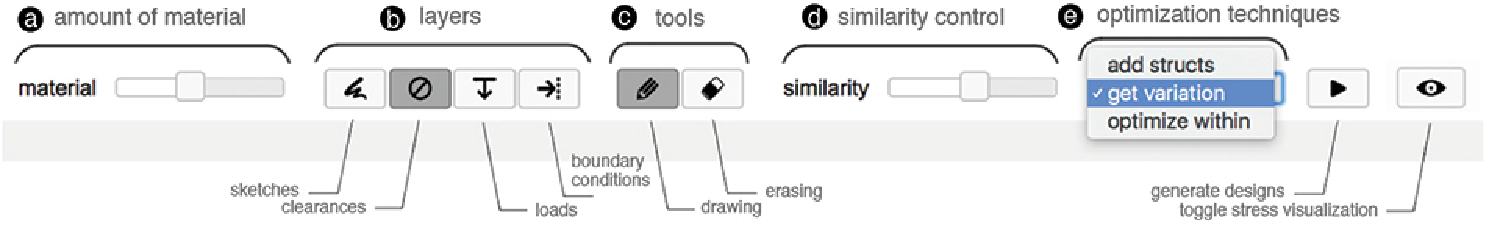
\includegraphics[width=1\textwidth]{figures/overview}
  \caption{Overview of Forte's default tool bar: adjusting the amount of material for generating the structures (a); different layers for sketching and specifying the loading scenario (b); drawing and erasing tools (c); controlling how the generated results are similar to the original sketch (d); and selecting different design optimization methods (e).}~\label{fig:overview}
\end{figure*}

%Validation
We envision Forte will empower professionals who design structures, such as industrial designers, mechanical engineers and architects. To validate our approach, we held design sessions with 10 participants. Our study demonstrates that Forte empowers designers to create and explore a range of optimized designs with custom forms and styles. While our current focus is on a 2D design tool, we showcase three post-processing techniques using external tools to turn a 2D design to a 3D object: \textit{extrusion}, \textit{warping} and \textit{combination}. We report stress analysis on these 3D models under varying loading conditions and finally demonstrate a series of fabricated examples.


\begin{figure} [h]
  \centering
  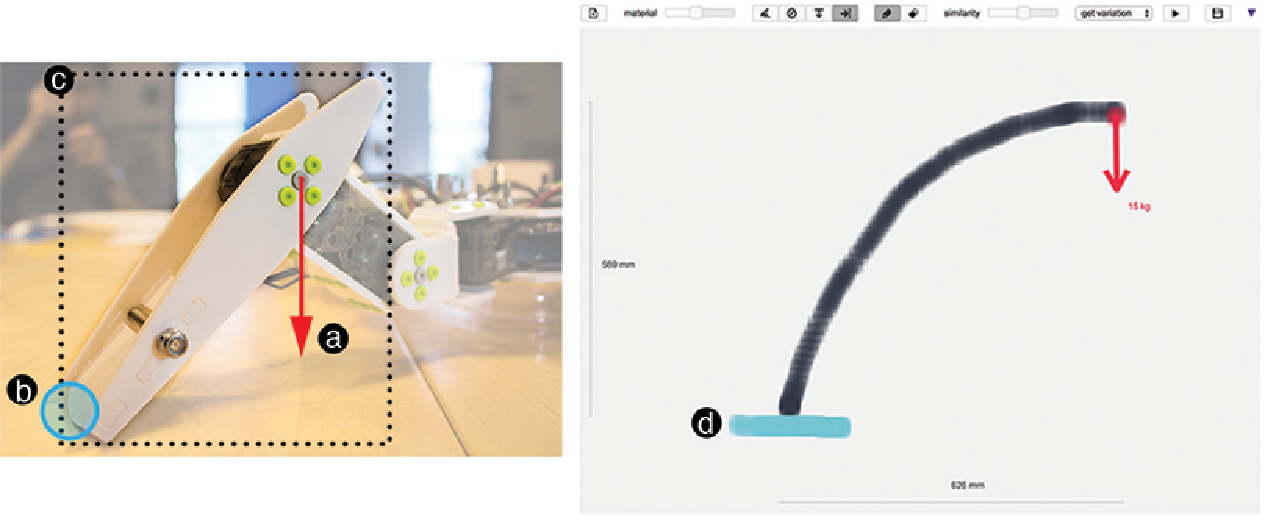
\includegraphics[width=0.75\textwidth]{figures/design_scene}
  \caption{From users' sketch, Forte (right) generates lightweight structures to support loads, such as a robot leg (left) that needs to support the robot's weight using a specified amount of material.}~\label{fig:design_scene}
\end{figure}

\section{Forte: User-Driven Generative Design}

\begin{figure*} [t]
  \centering
  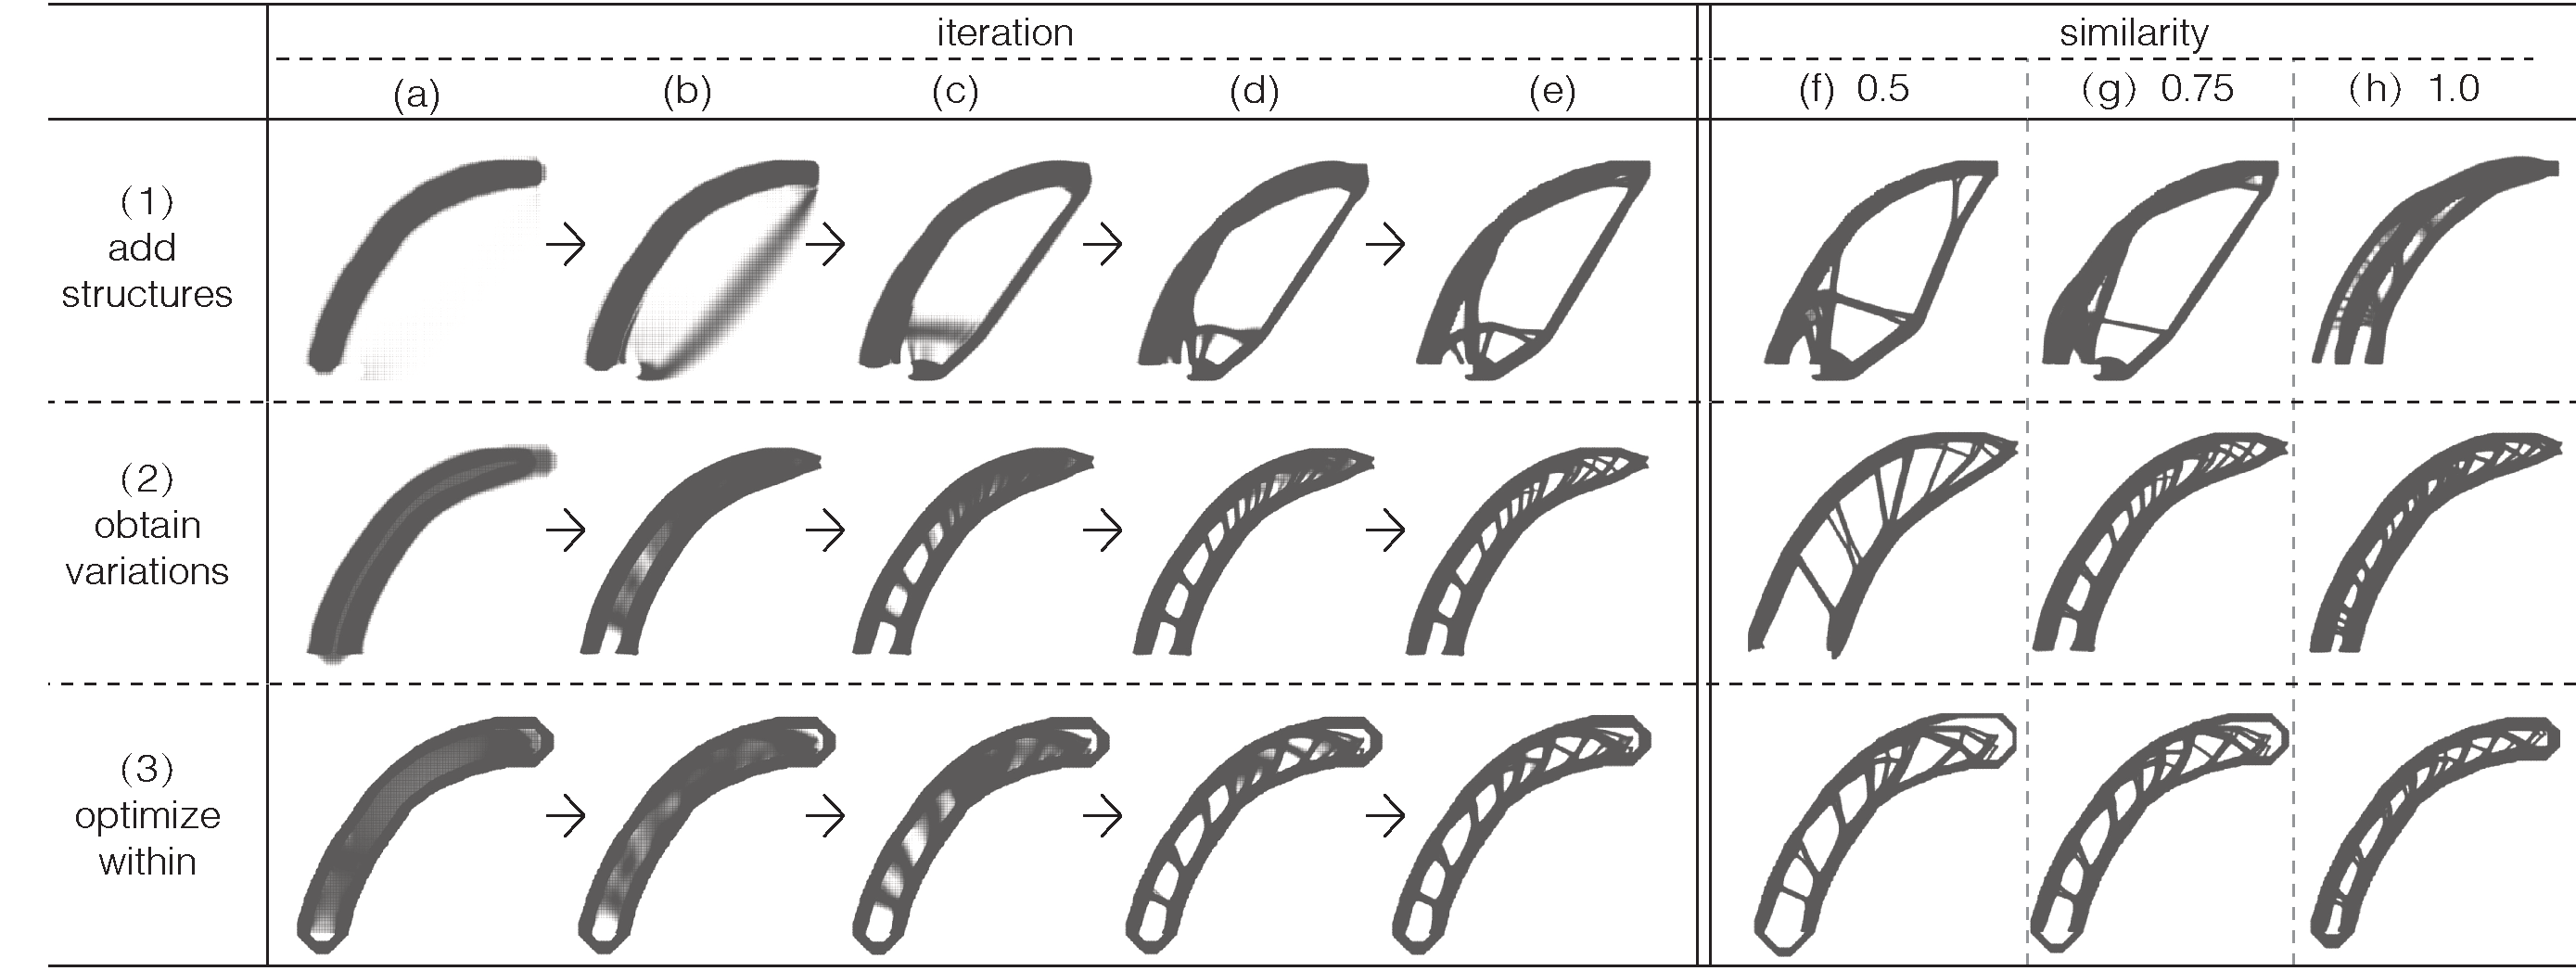
\includegraphics[width=1\textwidth]{figures/all_the_techniques}
  \caption{Forte's three types of design optimization iteratively generate structures based on user's sketch while providing them with real-time visual feedback akin to an animiation (a-e), the result of which can be controlled by a global `similarity' value (f-h).}~\label{fig:techniques}
\end{figure*}

In this section, we describe users' interaction with Forte and its key features for user-driven generative design, while leaving the technical details for later in the next section. Specifically, we will walk through a usage scenario: creating a 2D design of a leg for a quadruped robot (Figure~\ref{fig:design_scene}). The design goal is three-fold: {\em (i)} in contact with the ground (Figure~\ref{fig:design_scene}b), the leg needs to be optimized for supporting the weight of the robot's body (Figure~\ref{fig:design_scene}a), {\em (ii)} it needs to be lightweight to ensure the overall efficiency of the robot, and {\em (iii)} its form also needs to be customized with respect to other user-defined goals such as aesthetics. Below we first go through some basic concepts and terminologies and then demonstrate how Forte allows users to jointly achieve these goals.

\subsection{Basic Concepts and Terminologies}
Generative design via topology optimization considers an object as a distribution of a certain amount of material in order to meet certain performance criteria. This paper focuses on structural performance, which is optimizing structures---with only a limited amount of material available---to support a given load. For instance, a robot leg should be designed to support the weight of the robot's body with a lightweight structure. In Forte, a design consists of a sketch (considered below) and a \textbf{loading scenario}, which include {\em(i)} where the expected \textbf{loads} are and how large they are, and {\em(ii)} \textbf{boundary conditions}, which is where the object is in contact with its environment (e.g., a robot leg will touch the ground, as shown in Figure~\ref{fig:design_scene}). Based on this input, Forte will then generate structures via different types of \textbf{design optimization}, i.e., distributing allocated material in a structurally optimized way. Each type of optimization is also constrained by a given \textbf{amount of material}, which is typically measured by the percentage of the entire \textbf{design domain}--the bounding box of the design object (Figure~\ref{fig:design_scene}c). For example, 30\% material means the material used for the robot leg amounts to 30\% the size of its bounding box\footnote{We discuss later in the design sessions that participants found this to be a problematic way of measuring material, as it seems hard to get an intuitive estimate based on bounding boxes.}.

\subsection{Sketching Designs and Loading Scenarios}
With Forte, a user sketches a design idea as well as the loading scenario. Each type of sketch is drawn in a different color on its own layer (Figure ~\ref{fig:overview}b). This allows users to select and focus on one particular layer at a time. Once a layer is selected, it is pushed to the top with the rest of the layers set to semi-transparent.

\begin{figure} [h]
  \centering
  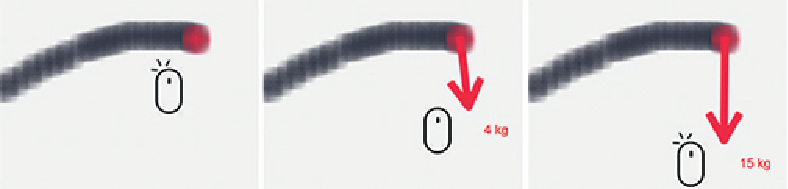
\includegraphics[width=0.7\textwidth]{figures/draw_load}
  \caption{Interaction to specify a load.}~\label{fig:draw_load}
\end{figure}

To start, a user simply selects the design layer and sketches a curve representing the robot's leg. With Forte, it suffices to provide such a simple representation that succinctly expresses the user's high-level design intent, i.e., ``I want the robot's leg to curve like this''. As the user sketches the robot leg, Forte also shows the dimensions of the current sketch's bounding box to inform users of the size of their design. The default scale is 20 mm per pixel, which can also be adjusted by the user in the preference settings.

As a next step, the user would consider the loading scenario. First, to create a load, the user switches to the load layer (Figure~\ref{fig:overview}), They can click on the sketch to indicate a single loading point, or draw to specify a sequence of loading points. As shown in Figure~\ref{fig:draw_load}, as soon as these points are drawn (e.g., mouse released), an arrow is rendered, following the cursor (e.g., where the mouse moves), and indicating the direction as well as the amount of load, which is also shown at the end of the arrow. A click confirms and pins down this load vector. To specify a boundary condition, the user simply draws it on the corresponding layer (Figure~\ref{fig:design_scene}d).

In addition, Forte also supports a fourth type of layer that allows users to lasso-select a \textbf{clearance} region that needs to be kept clear, e.g., the space above a chair's seat or around the tip of a hook (Figure~\ref{fig:draw_clearance}). This information proactively prevents generating structures at places that will compromise the usage of an object.

\begin{figure} [h]
  \centering
  \vskip 4pt
  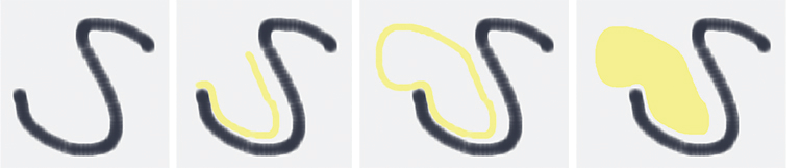
\includegraphics[width=0.7\textwidth]{figures/draw_clearance}
  \caption{Lasso-selecting an area of clearance around the tip of the hook (no structure generated here).}~\label{fig:draw_clearance}
\end{figure}

\begin{figure*} [t]
  \centering
  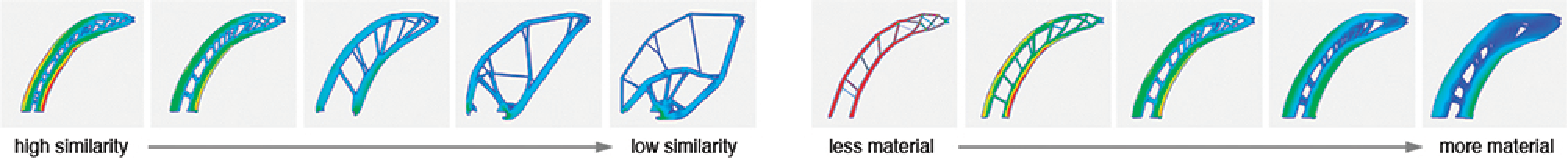
\includegraphics[width=1\textwidth]{figures/sim_mat}
  \caption{Stress visualization informs performance trade-off between different similarity values (left), and the amount of material (right).}~\label{fig:sim_mat}
\end{figure*}

\begin{figure*} [t]
  \centering
  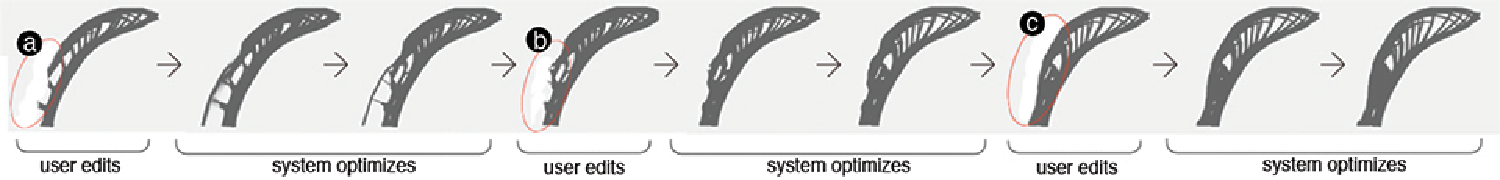
\includegraphics[width=1\textwidth]{figures/local_editing_eraser}
  \caption{Users can suggestively erase part of a generated result (ab), which prompts the system to update the optimization addressing the intent of removing material; with this tool, users can also refine or smoothen a generated result (c).}~\label{fig:local_editing_eraser}
\end{figure*}

\subsection{Design Optimization with Global Similarity Control}

Once the user creates a sketch and specifies the loading scenario, they can now explore three different ways the system can generate structures by design optimization. Forte considers the generation of structures  as a spectrum between users' original idea and the system's solution to the defined problem. Users can navigate on this spectrum by adjusting a \textit{similarity} value from 0 to 1 (Figure~\ref{fig:overview}d): conceptually, a low similarity would allow the system to `deviate' more from the user's initial sketch while a higher value will keep the generated structures closer to what the user originally draws. Further, Forte's optimization algorithms run at an interactive rate, providing users with real-time visual feedback after each iteration, as demonstrated in the accompanying video figure.
% As shown in Figure \xx, a design with $375\times323=121,125$ finite elements can be generated in less than two minutes. 
Below we illustrate Forte's three new generative design optimizations and how similarity allows users to have direct control of the generated results.

% \begin{figure*} [t]
%   \centering
%   \includegraphics[width=2\columnwidth]{figures/gv_similarity}
%   \caption{Obtain variations: as similarity increases (a$\rightarrow$e: 0, 0.25, 0.5, 0.75, 1.0), generated variations follow the user's sketch more closely; turning on the stress visualization shows the structural tradeoff.}~\label{fig:gv_similarity}
% \end{figure*}

\textbf{Add structures} \hspace{0.1cm} To start, Forte can generate additional structures to strengthen the user's original sketch. For example, as shown in Figure~\ref{fig:techniques}(1a-1e), a major truss structure is added parallel to the user-sketched robot leg as reinforcement. 

%\begin{figure} [h]
%  \centering
%  \includegraphics[width=1\columnwidth]{figures/add_structs}
%  \caption{Add Structures: generating additional structures (a$\rightarrow$e) for the robot leg to strengthen the user's original sketch (this trial: 121,125 elements, 30 iterations, 3.45 sec. per iteration).}~\label{fig:add_structs}
%\end{figure}

The similarity value effectively controls how far away from the original sketch these structures can be added. As the user increases similarity, added structures will appear increasingly closer to the original sketch and eventually become part of it, equivalent to a thickening operation (Figure~\ref{fig:techniques}(1h)). However, note that the added structures' position does not change smoothly with the similarity value; rather it tends to `snap' to positions along the way that are structurally meaningful. 
% SEH: seems ok to me \xac{not sure the last sentence is understandable}

Overall, `add structures' is targeted at situations where users only have a partial or incomplete design idea in mind and are unsure whether and how they should add extra structures to provide support for the loads.

%\begin{figure} [h]
%  \centering
%  \includegraphics[width=1\columnwidth]{figures/as_similarity}
%  \caption{Add structures: as similarity increases, added structures emerge closer to the original sketch (similarity value a$\rightarrow$e: 0.5, 0.75, 1.0). }~\label{fig:as_similarity}
%\end{figure}

\textbf{Obtain variation} \hspace{0.1cm} Forte provides a second optimization algorithm that can generate variations of the initial sketch. For example, as shown in Figure~\ref{fig:techniques}(2a-2e), Forte generates two parallel interconnected trusses instead of one user-sketched structure; however, the variation still bears resemblance to the original sketch as it globally follows the curve path specified by the user. As the user increases the similarity value, the generated structures will follow the user's sketch more closely (Figure~\ref{fig:sim_mat}). `Obtain variation' works best when users only have a concept (e.g., a skeleton) of what the design should look like without any structural details, in which case the system will take the initial designs as `seeds' and vary it with generated structures.

%\begin{figure} [h]
%  \centering
%  \includegraphics[width=1\columnwidth]{figures/get_variations}
%  \caption{Obtain variations: generating a variation (a$\rightarrow$e) of the initial sketch to improve the structural integrity (this trial: 121,125 elements, 30 iterations, 2.91 sec. per iteration)}~\label{fig:get_variations}
%\end{figure}

\textbf{Optimize within} \hspace{0.1cm} Forte can also consider the user's sketch as solid shapes (rather than skeletons) and optimize the internal structures within. For example, as shown in Figure~\ref{fig:techniques}(3a-3e), Forte reproduces the contour of the user-sketched robot leg while filling in generated structures. By controlling similarity, the user can effectively shrink or expand the contour, e.g., decreasing similarity results in a robot leg of the same curvy shape but much thicker than the original sketch, given the system more space to generate structures. `Optimize within' serves well for cases where users already have a fully-designed solid shape but want to re-design the interior structures.

%\begin{figure} [h!]
%  \centering
%  \includegraphics[width=1\columnwidth]{figures/optimize_within}
%  \caption{Optimize within: expanding user sketch into a contour and generating (a$\rightarrow$e) internal optimized material layout (this trial: 121,125 elements, 30 iterations, 2.87 sec. per iteration).}~\label{fig:optimize_within}
%\end{figure}
%
%\begin{figure} [h!]
%  \centering
%  \includegraphics[width=1\columnwidth]{figures/ow_similarity}
%  \caption{Optimize within: lowering similarity expands the contour of the user sketch, allowing more room for optimization to generate structures (similarity value a$\rightarrow$c: 3.5, 5, 7.5).}~\label{fig:ow_similarity}
%\end{figure}

For any of these design optimizations, users can adjust how much material can be used in generating the design. For example, as shown in Figure~\ref{fig:sim_mat}, reducing the material amount often creates hollow structures with trusses, while a higher value tends to thicken or fill up certain parts of the design.

% \begin{figure*} [t]
%   \centering
%   \includegraphics[width=2\columnwidth]{figures/gv_material}
%   \caption{Reducing the material amount often creates hollow structure with trusses, while a higher value tends to thicken or fill up certain parts of the design (amount of material a$\rightarrow$e: 5\%, 10\%, 15\%, 20\%, 25\%).}~\label{fig:gv_material}
% \end{figure*}

As the user runs one of the three optimizations, Forte creates and records a trial, and together displays a history of results from all these trials. Selecting a trial not only shows the resulted structures, but also updates the menu so that users can see which of the three optimizations was used, how much material was allocated and what similarity value was applied.


\begin{figure} [b]
  \centering
  \includegraphics[width=0.75\columnwidth]{figures/local_editing_pencil}
  \caption{Users can suggestively add material to a generated result (circled strokes), which prompts the system to re-run the optimization and attempt to add structures accordingly.}~\label{fig:local_editing_pencil}
\end{figure}

\subsection{\#3 Refining Optimization with Local Suggestive Edits}
The similarity value allows users to control the optimization outcome at a global level with respect to the entire design. Complementarily, once a result is generated, users can also perform fine local editing, which will prompt the system to re-run the optimization, taking into account users' underlying intent of the edit. For example, if a user wants a thinner tip of the robot leg, they can use the eraser tool (Figure~\ref{fig:overview}c) to scrub that area (Figure~\ref{fig:local_editing_eraser}a, shadowed part). The system immediately starts a new optimization and returns an updated result with less material on the tip of the leg. Increasing the erasing `power' and applying it again finally sharpen the leg, but results in a rough outline (Figure~\ref{fig:local_editing_eraser}b). We can also use this tool to smooth the optimized result (Figure~\ref{fig:local_editing_eraser}c).

Similarly, the user can also use the pen tool (Figure~\ref{fig:overview}c) to draw on an optimization result, such as adding a truss to the leg (Figure~\ref{fig:local_editing_pencil}ab). The system will also re-run the optimization and will attempt to generate some structures where the new truss is drawn (Figure~\ref{fig:local_editing_pencil}).

This technique is called suggestive editing, as users' action do not directly remove or add to the design; rather, it serves to suggest their intent to the system, e.g., ``I want less material here'', or ``I would like to add something there''. The next round of structure generation will take into account such intent and attempt to realize it through the optimization process. However, intent cannot be realized if the removal or addition of material compromises the structural integrity of the design (e.g., removing the entire bottom part of the robot leg, making it unable to stand on the ground).

\subsection{\#4 Informing Performance Trade-offs with Visualization}
As users exploratively customize the optimization process, it is important to inform them of the performance trade-offs. Forte allows users to toggle a stress visualization (Figure~\ref{fig:overview}) overlaying each optimized result (Figure~\ref{fig:sim_mat}) . The heat map indicates which part of a design is the weakest; it also allows users to compare different designs' performance and see how the stress situations evolve as the design evolves. Users can also adjust the safety factor: a higher value is equivalent to assuming more weight, thus revealing more structurally problematic areas in the design.
 
% \pagebreak

\section{Implementation}
In this section we describe technical details of Forte's implementation. 

\subsection{Sketching Designs and Loading Scenarios}
Recall that users' design input consists of a sketch within a design domain as well as loads, boundary conditions (Figure~\ref{fig:design_scene}), and/or clearance (Figure~\ref{fig:draw_clearance}).

Given these input parameters, first the design domain is discretized into $N=W \times H$ square \textbf{finite elements} \cite{zienkiewicz1977finite}, each of which (denoted as $e$) is assigned a \textbf{density} value $x_e \in [0, 1]$. The user's intial sketch is discretized into a binary density map on this domain with 1's for elements overlapping with the sketch and 0's for the others. Similarly, loads, boundary conditions and clearance are also converted to such density maps.  In addition, for loads each density=1 element is also associated with a load vector indicating the amount of the load as well as the direction. 

% Specifically, if users draw a sequence of load points, we divide the load vector across all the points so that $\Sum{\mathbf{n}_j \dot \mathbf{f}_j}/=\mathbf{f}$, where $\mathbf{n}_j$.
%
% \xac{explain why fitting circle}

\subsection{Design Optimizations with Global Similarity Control}
The implementations of the three design optimization techniques presented here are developed based on the 88-line program \cite{andreassen2011efficient}, which uses a SIMP (Solid Isotropic Microstructure with Penalization) method for topology optimization. For readers to better understand our approach, we first provide a brief of overview and refer the reader to Andreassen et al. for further details \cite{andreassen2011efficient}.

Overall, the process solves the following compliance optimization problem:
\begin{equation}
	\min_x: c(\mathbf{x}) = \mathbf{U}^T\mathbf{K}\mathbf{U} = \sum^N_{e=1} E_e(x_e)\mathbf{u}_e^T\mathbf{k}_0\mathbf{u}_e,\\
\end{equation}
	subject to:
\begin{gather*}
	{V(\mathbf{x}) / V_0} \leq f ; ~~ 
	\mathbf{K}\mathbf{U} = \mathbf{F};  ~~
	0 \leq x_e \leq 1
\end{gather*}
where $c$ is the compliance of the design, which is computed with $\mathbf{U}$ -- the global displacement matrix, and $\mathbf{K}$ -- the global stiffness matrix determined by the stiffness of the material as well as its distribution (or layout). The objective function is further broken down to the summation of compliances across all elements: $E_e$ is the Young's modulus of $e$ ($E_e = E_{min} + x_e^p(E_0 - E_{min})$), $\mathbf{k_0}$ is the unit stiffness matrix which together with $E_e$ determines the stiffness of element $e$; $u_e$ is the displacement vector of $e$. Finally, $\mathbf{U}$ can be computed from $\mathbf{K}\mathbf{U} = \mathbf{F}$, where $\mathbf{F}$ is vector of forces (loads).

% \begin{equation}
% x_e^{new} = optimize(x_e) = {{1 \over {\sum_{j \in N_e}{H_{ej}}}}} \sum_{j \in N_e}{H_{ej}x_e}
% \label{eq:opt_xe}
% \end{equation}

At each iteration, once $c$ is computed, $x_e$ is updated as follows:
\begin{equation}
% \begin{aligned}
	x_e^{new} = 
	\begin{cases}
    max(0, x_e-m),	& \text{if } x_eB_e^\eta \leq max(0, x_e-m) \\
    min(1, x_e+m),  & \text{if } x_eB_e^\eta \geq min(1, x_e-m) \\
    x_eB_e^\eta 	& \text{otherwise}
	\end{cases}
% \end{aligned}
\end{equation}
where $m$ is a pre-set step for density changes, $\eta = 1/2$ is a numerical damping coefficient, and $B_e = (-{\partial c \over \partial x_e})/(\lambda{\partial V \over \partial x_e})$, with $\lambda$ being a constraint factor to ensure the total volume does not exceed $V_0f$---the allocated amount of material where $f$ is the percentage and $V_0$ is the volume of the design domain.

% cite: stress relife; guided exploration
% \subsection{Types of Design Optimizations with Controlled Similarity}
% [figure] the part of the ui with the three options

This process represents the classic topology optimization approach that automates the generation of structures in a `black box'. Below we describe our methods of extending it to a user-driven approach, allowing the control of the optimization results via a similarity value.


\textbf{Add structures} \hspace{0.1cm}
We initialize the design domain by assigning each element the value of $f$
%the specified amount of material 
(e.g., 15\% of the bounding box area). Through iterations the optimization will increase or decrease this value for a given element, thus forming a global structure. After each iteration, we add the intermediate generated structures to the user's sketch, and take it as the input for the next iteration. Specifically, now each element density is computed as
\begin{equation}
    \widehat {x_e^{new}}= 
\begin{cases}
    1,          & \text{if } e \in user~sketch\\
    x_e^{new}	& \text{otherwise}
\end{cases}
\end{equation}
To control similarity, we perform a \textit{mass transport} (cf. \cite{bonneel2011displacement}) after each iteration before adding the intermediate results to the user's sketch. A mass transport considers two designs (e.g., user sketch vs. optimized result) as two ways of distributing the same amount of mass (computed by summing up elements' density), and transports the mass in between the two distributions to obtain an interpolation. We use mass transport to interpolate between the optimized result and the user sketch, taking similarity as the weight of interpolation (0: user sketch --- 1: optimized result). This allows us to control how much the design will be similar to the original sketch after adding the optimized result.

We implement the mass transport function by computing and interpolating the barycenters of the two input designs as distributions. We compute the distance field of the user sketch and use it as the input distribution to the mass transport function. This provides more fine-grained information at each element (what is the distance of this element to the user sketch) beyond a binary value (whether or not it is part of the user sketch).

\textbf{Obtain variation} \hspace{0.1cm}
Instead of $f$, we initialize the design domain with the user's sketch, and then run topology optimization, which will effectively `shift' the material away from user-specified locations to achieve a variation with optimized material layout.

%To control similarity, we first experimented with the same mass transport approach. However, it tends to `oscillate' between user sketch and the optimized result, and takes long to converge. Before this problem did not occur, which we hypothesize is because it is operating on a smaller `delta' between user sketch and optimized result (at n+1 th iteration, the result is optimized from the n th iteration's added to user sketch). 
%
%Thus we take a different approach, focusing on controlling similarity right from the input. Specifically, we map the distance field of the user's sketch to the input design domain as 
To support user control of similarity,  we map the distance field of the user's sketch to the input design domain as 
\begin{equation}
x_e^{initial} = {1\over \sum_{i=1}^N{cos({{\pi d(i)}\over 2})^s} }cos({{\pi d(e)}\over 2})^s f
\end{equation}

where $x_e^{initial}$ is the initial material density at element $e$, $d$ is the normalized distance field function, $s$ is the user specified similarity request, and the $cos$ function raised to $s$ produces value close to 1 when $d(e)$ is small (close to the user's sketch) and drops rapidly to 0 when shifting away. $s$ controls how quickly such a drop occurs. Thus a larger similarity value will initialize the optimization (hence the result as well) more closely to the user's sketch, while a smaller value will loosen the constraint by `diluting' the user's sketch, and produces a result with wilder variation.

% One limitation of this approach is that if part of the user's sketch is considered `unnecessary' (i.e., not providing structural support), the optimization will tend to reduce a larger chunck of it, resulting a disproportional dissimilarity to the original design. To provide an alternate approach which avoids this problem, we introduce the following method that always keeps the shape of the user's sketch and optimizes the structure within.

\textbf{Optimize within}
We consider the user's sketch as a `skeleton'. As a first step, we expand it using the distance field by setting a new contour around the original sketch. We then run the optimization only within the contour, as follows, at each iteration,
\begin{equation}
    \widehat {x_e^{new}}= 
\begin{cases}
    x_e^{new},	& \text{if } d(e) < d_c\\
    1,              		& \text{if } d_c \leq d(e) < d_c + t\\
    0 						& \text{otherwise}
\end{cases}
\end{equation}
$d_c$ is a distance field value used to define the new contour, and $t$ controls the thickness of the contour. We control similarity by shifting $c$ towards or away from the user's original sketch.

% \textbf{Comparing the three design optimizations}
% ...

% \subsection{Controlling Global Similarity}

\subsection{Refining Optimization with Local Suggestive Edits}
% As users perform the initial sketch and run it through the above design optimization, they might expect to edit the results. 
Forte enables users to interactively suggest adding to, or removing from, parts of the optimization result, which then prompts the system to re-run the optimization to produce a version that matches the users' intent, including the new edits. Importantly, in such re-run, the system is initialized based on the result from the previous run, rather than starting from the original sketch.

As a user draws on, or erases, parts of a design on a $W \times H$ domain, we create a mask $M$ of the same dimensions with each pixel's value $M_e \in [1-\Delta_{remove}, 1+\Delta_{add}], \Delta_{remove} \in (0, 1), \Delta_{add} > 0$. Then in the optimization process, we update element $e$ as
\begin{equation}
\widehat {x_e^{new}}=M_e x_e^{new}
\end{equation}
In essence, $M_e$ indicates whether and how much a user would want to add or remove material at this point.
% \begin{equation}
%     x_e^{new}=M_e \, optimize(x_e)
% \end{equation} 
If a user performs an erasing action, $M_e$ is set to be in $[1-\Delta_{remove}, 1)$, which will dampen the to-erase elements' density at each iteration; if a user performs additional drawing, we integrate the addition to the result as input for the re-run. As $M_e$ is now set to be in $(1, 1+\Delta_{add}]$, it will amplify the to-add elements' density at each iteration. All unedited $M_e$'s will be set to 1.

% Further, we also allow users to control whether to erase or add material percisely at some locations, or more loosely in a certain area. This is enabled by smoothing $M$ using a variable Gaussian kernel. 

\subsection{Informing Performance Trade-offs with Visualization}
We compute the von Mises stress of each optimized result using Biyikli and To's method \cite{biyikli2015proportional}, which is implemented as an integral component of the optimization process. The values in the stress distribution are then normalized by a material-specific yield stress $\sigma_y$ and visualized as a heat map. All our examples and demonstrations in the design tool use a material model based on an Extrusion Grade PLA \cite{NatureWo45:online}. The yield stress is also divided by the user-specified safety factor, e.g., a $2\times$ safety factor will result in the use of $\sigma_y/2$, thus visually revealing more potentially problematic area in the design.

\subsection{Software and Hardware}
The front end of Forte is written in JavaScript using jQuery\footnote{jQuery: \url{https://jquery.com/}} for UI development. The back end consists of two components: {\em(i)} the optimization techniques were written in MATLAB, which is then compiled into a standalone service; and {\em(ii)} a phython-based server which relays optimization requests and input parameters from the front end to the MATLAB service, and sends back the results. Everything runs on a MacBook Pro (Retina, 15-inch, Early 2013) with a 2.4 GHz Intel Core i7 and 8 GB 1600 MHz DDR3 memory. In our demonstrations, the front end runs on a Google Chrome web browser.

\section{Design Sessions}
To validate Forte, we conducted informal, qualitative design sessions with 10 participants. The objective of the study is to let participants create their own designs using Forte's user-driven generative approach, and elicit their initial reaction and feedback to the system to reveal existing problems and to inform future improvements.

\subsection{Participants}
We recruited 10 participants from our university (1 female, aged 18-33). Two majored in interaction design, three in architecture and the others in mechanical engineering. All participants reported to have sketching experience and all had experience using CAD tools. Two reported to be knowledgeable about topology optimization, four had passing knowledge and the others had none.

% \subsection{Design}
% We employed a within-subject design with an independent variable of \textit{Technique}. We compare two techniques: Forte and a baseline--a conventional topology optimization system where users can only specify loads, boundaries and the amount of material. Participants used the techniques to conduct two sessions of design tasks to create a total of 8 objects. The order in which they accessed the techniques was counter-balanced. The set of objects were also different between techniques to prevent carry-over effect.
 % (i.e., for each participant we avoided designing the same object twice using different techniques. 
% Thus we devised Object as a between-subject variable.
% Overall, permutation resulted in a 8x8 latin square design as shown in Figure xx.
% The order in which they accessed the techniques was counter-balanced. To prevent carry-over effect, we avoided designing the same object using both techniques. Thus we devised Object as a between-subject variable. Permutation resulted in a 8x8 latin square design.

\subsection{Tasks \& Procedure}
The design sessions took place in our research lab and lasted between 1 and 1.5 hours for each participant. To begin, participants were given a tutorial by the experimenter on some basic understanding of topology optimization, and how to use Forte by walking through a concrete example of designing a bracket. Next, they were asked to use Forte to create objects of their own design, as well as coming up with loading scenarios. For each design, they were free to choose any of the three optimization techniques and run as many trials as they would like. Participants created 2-4 designs during the course of the study.
% Participants could decide what to design, or to choose from a list provided by the experimenter. 
% For each object, the experimenter described the functional requirements (loads and bondary conditions), such as ``a chair with a load on the back for a person to lean on, a load on the bottom for sitting, and boundary condition on the ground''. We felt that such detailed guidance was necessary for these non-expert users who experienced topology optimization for the first time. Once an object was described, the participant was asked to create and explore as many designs as they desire, and select up to five as their favorites.

Throughout the design session, participants were asked to think aloud as the experimenter took notes. they completed a questionnaire to summarize their experience with Forte, e.g., what they like about the tool, what problems they encountered, and what new features they would like to have in the future.


% \subsection{Apparatus}
% The baseline system used in the study only had a subset of Forte's feature. Thus we implemented it as a simplified version of Forte. Both systems ran on a ... with a Wacom stylus connected to provide a more natural way of performing sketching. After the study, we used machines described in Section XX to fabricate participants' designs.

\subsection{Feedback and Discussion}
We analyzed the qualitative data using a method akin to the Affinity Diagram approach \cite{beyer1997contextual}. We organized notes of participants' comments and survey response to iteratively develop meaningful and coherent themes. 

Overall, participants responded positively to Forte's user-driven generative design approach: ``I like how it can produce interesting shapes, i.e., organic, asymmetric shapes which are difficult/time-consuming to hand-draw'' (P1); ``... pretty nice about making the idea of topology optimization accessible to people'' (P5); ``computer generating structures from my sketch is interesting; it might be the way computers can design something like humans do in the future'' (P10).

\textbf{Optimization techniques} \hspace{0.1cm} Participants were able to learn and recognize the difference between the three optimization techniques. Further, some developed their own understanding and preferences of the techniques. For example, P1 mentioned that ```add structures' lead to traditional shapes; `obtain variation' is more creative.'' P4 liked to use `add structures' as he wanted ``the system to add something different from the original drawing''. P9 extensively used `optimize within' as he wanted to keep the exact shape of the drawing and only optimize what is inside.

\textbf{Similarity control} \hspace{0.1cm} Participants had no trouble understanding or using the similarity control. P1 commented that ``... it allows me to control how much imagination I need''. P4 liked that he could control how different the result will look from the original design. P7 summarized the experience of controlling similarity as having ``design freedom'', and felt he ``can design anything and [Forte] will keep it to some extent [after optimizations]''.

\textbf{Real-time feedback} \hspace{0.1cm} Participants found it pleasant and useful to see how the design evolved in real time: ``[I] enjoy watching the shape evolving'' (P1), ``Watching it grow and iterate is really nice--it helps you visualize stresses and know where the strength needs to be'' (P2), ``It helps a lot to see how things are branching out, happening in the background'' (P7).

\textbf{Local suggestive editing} \hspace{0.1cm} We observed only three participants frequently used local suggestive editing. They all appreciated this capability of refining the optimized design: ``... very easy to make quick changes on the fly to see how overall structures change'' (P2); ``... add and subtract material dynamically which was very helpful'' (P7). P10 would continuously use this feature in a sequence of trials to add more reinforcement based on the stress visualization.

\textbf{Existing problems and suggested features} Participants also pointed out existing problems and suggested new features in the tool. One main confusion is the amount of material: P2, P4 and P5 thought it was relative to the sketch, whereas it was actually relative to the sketch's bounding box. P5 also suggested visualizing the actual size of allocated material to give users a more concrete idea. Four participants (P2, P4, P7 and P10) asked how they can `transfer' an optimized result to the original drawing, or simply just be able run technique B on technique A's result. Such request points to an interesting problem for future work, which is enabling users to manage how an initial design branches out to a complex tree structure. Finally, participants proposed other controls akin to the similarity variable, e.g., keeping the design balanced (P1), controlling the global maximum thickness of the generated trusses (P5), and specifying symmetric structures (P6, P7), all of which suggest fertile opportunities for future work.

\subsection{Designs Created by Participants}
Figure~\ref{fig:participants_design} shows a series of designs created by the participants. Overall, we observe two recurring approaches of creating these designs. First, some users would take a `form-first' approach, whereby they started by drawing their imagined form and then drove the system to generate structures similar to the form. For example, `public bench' by P1 (Figure~\ref{fig:participants_design}a) started with a single curve as a shared sitting space, while the system generated structures underneath to support it. `Cross-legged book case' by P6 (Figure~\ref{fig:participants_design}e) started with a form that almost looked like a Small Seal Script\footnote{Small Seal Script. \url{https://en.wikipedia.org/wiki/Small_Seal_Script}} character in ancient Chinese. In contrast, other users would take a `structure-first' approach, starting with a basic structure based on the object's functionality; they explored which of the system's generated structures can also create interesting forms to the design. For example, `eagle crane' by P2 (Figure~\ref{fig:participants_design}f) was initially drawn as a simple polygon that provides the functionality of a crane. However, as the system `morphed' the input structure, it evolved into an eagle head shaped design. `House' by P8 also started with simple geometry representing a two-story house, a loft and a patio, which then evolved into two distinct design variations (Figure~\ref{fig:participants_design} g and h, using `obtain variation' and `add structures', respectively).


We also observed different iteration strategies. Most users iterated a design by playing with different similarity values and amounts of material. For example, P3 used Forte to design (the cross-section of) the GE Aircraft Engine Bracket (Figure~\ref{fig:participants_design}c). His first three trials were simply trying out different material-similarity combination to gauge variety of the underlying design space. 
% On average, users ran XX optimization trials for a design before switching to a different optimization or finishing the current design. XX\% of the time users only tried one optimization technique, XX\% of the time they switched to a different one, and only XX\% of the designs went through all three techniques.
% https://sffsymposium.engr.utexas.edu/sites/default/files/2014-110-Carter.pdf
Finally, quite a few users modified their initial design based on the system's generated structures. For example, in designing a bike frame (Figure~\ref{fig:participants_design}b), P2 noticed that the system did not keep one of the trusses he drew but instead created a different one. P2 then modified the initial design to a `imitate' the system's approach. Participants also tried to modify the system's design. As mentioned above, three participants were observed actively using the local editing techniques. For example, In designing a bow P7 used the eraser tool to iteratively refine the shape of the bow updated by the system ((Figure~\ref{fig:participants_design}d).

Figure~\ref{fig:participants_design} shows other designs created by our participants.

\begin{figure} [h!]
 \centering
 \includegraphics[width=0.6\textwidth]{figures/participants_design}
 \caption{Designs created by 10 participants using Forte.}~\label{fig:participants_design}
\end{figure}


\section{Post-processing and Fabricated Results}
Forte enables users to formulate, express and optimize their design in a 2D environment. To  fabricate their designs into 3D artifacts, we describe three post-processing techniques using external tools (e.g., the Rhinoceros\footnote{\url{https://www.rhino3d.com/}} CAD system) for fabrication and showcase some of the fabricated results.

\begin{figure} [h!]
  \centering
  \vskip 8pt
  \includegraphics[width=1\textwidth]{figures/result_collage}
  \caption{Fabricated examples designed from Forte's generated structures: legs for a quadruped robot (a); a bike seat (b); an S-shaped chair (c); high heels (d); pet jumping platforms (e); a reading chair (f); and a tea table (g).}~\label{fig:result_collage}
\end{figure}


\begin{figure*} [t]
  \centering
  \includegraphics[width=1\textwidth]{figures/results}
  \caption{All our fabricated examples from the sketches in Forte, to generated 2D designs, and to post-processed 3D models; we performed a Finite Element Analysis on each 3D model based on the input loading scenario, which shows consistent stress distribution across a range of increasing loads.}~\label{fig:results}
\end{figure*}

\textbf{Extrusion} We can extrude a 2D design along a path to create a 3D object. First we convert a generated design from a bitmap to a vector graphic, which can already be used in a laser cutter to create planar objects, such as the legs for the quadruped robot (Figure~\ref{fig:result_collage}a). Further we can also import the vector graphics to a 3D modeling tool for creating a 2D surface and extruding it to a 3D object. We use this technique to create a multi-functional reading chair that consists of an overhead light, a reclined sitting area, and bookshelves (Figure~\ref{fig:result_collage}f). Extrusion is not limited to a perpendicular path: for example, it is possible to extrude the 2D chair profile in Figure~\ref{fig:result_collage}c along a circular path to create a bench.

% robot leg
% reading chair

\textbf{Warping} We can also warp a 2D design into a 3D surface. We used this technique to design a pair of high heel shoes using generated structures as the base (Figure~\ref{fig:result_collage}d). We designed a jumping platform for chinchillas by warping the cross-section to form a rounder top (Figure~\ref{fig:result_collage}e). We designed a bike seat by warping a 2D generated pattern to the shape of a cushion (Figure~\ref{fig:result_collage}b).

% high heel shoes
% chinchilla platform
% bike seat

\textbf{Combination} We can join multiple planar components made from the 2D designs (e.g., fabricated using laser or CNC cutting) to create 3D structures. For example, we designed a tea table supported by two joined structures (Figure~\ref{fig:result_collage}g).
%This cup holder mounted on an arm rest is made from two different generated components combined together.

% cup holder
% coffee table



To test the structural integrity of the 3D models produced in the post-processing step, we performed Finite Element Analysis (FEA) using Autodesk Inventor \cite{AboutSha59:online}. As shown in Figure~\ref{fig:results}, we tested each model on a range of increasing loads---from normal to overloading---and found consistent stress distribution across all the cases with high structural performance\footnote{We define the range of loads based on the usage scenarios of each design. The heatmap visualization is based on the maximum stress amongst all five loads.}. As our current focus is on the 2D design tool, this test is only based on our current examples (as well as specific types of material chosen for running FEA). Further experiments are required in order to validate the general process of converting 2D structural patterns to 3D objects manufactured in a wide range of materials, which we leave as future work.

% \begin{figure} [h]
%   \centering
%   \includegraphics[width=1\columnwidth]{figures/results}
%   \caption{caption to be added.}~\label{fig:result_collage}
% \end{figure}
 
\section{Limitations, Trade-offs and Future Work}
We discuss limitations and trade-offs to better understand our current system, as well as pointing to potential future work.

\textbf{Going from 2D to 3D}
Forte is currently a 2D oriented tool, although our examples have shown three ways of extending it to 3D: extrusion, warping and combination. The implementation of Forte is also extensible to 3D: on the front end, prior work has demonstrated numerous techniques for enabling sketching in 3D \cite{igarashi2007teddy, bae2008ilovesketch, bae2009everybodylovessketch}; on the back end, the optimization can also handle 3D cases by adding a third dimension to the input parameters (design domain, loads, boundary conditions, etc.) as well as the material stiffness matrix. Perhaps the real challenge of going 3D is maintaining real-time feedback and interactive iteration. Past work has explored engineering solutions for handling 3D generative designs. For example, Aage et al. provide a topology optimization implementation based on PETSc (Portable and Extendable Toolkit for Scientific Computing), which enables incredibly fine discretization, e.g., a (3D) design with 27.6 million design elements running on 24 CPUs (144 cores) only requires 30-60s per iteration \cite{aage2014topology}. Building upon all this prior work, our next step will develop and extend Forte to a fully 3D design tool.

\textbf{Ambiguity and imprecision of sketching}
As mentioned in Gross and Do's work, sketching is a particularly appealing medium for early ideation and design formation, as it embraces ambiguity and imagination. As discussed in the design session, this is also a strength of Forte, as it allowed participants to use unique hand-drawn forms to generate structures. However, as pointed out by a few participants, Forte lacks support for more precise design, e.g., straight lines, smooth curves, and symmetry. In the future versions of Forte, we would like to add more controlled ways of specifying designs.

\textbf{Generating and exploring a large space of examples}
Currently each of Forte's optimized result is initiated and driven by the users. While this gives users freedom to explore and customize each optimization trial, it becomes a somewhat tedious process as the number of trial increases. In the future we plan to explore ways to automatically generate a large design space of structures from a single user input. To realize this, the challenge is two-fold: {\em(i)} how to infer and sample more variables from one single user input in order to generate more than one result; {\em(ii)} how to enable users to efficiently navigate and filter a large number of results. Our future work will explore solutions to tackle these two challenges.

\textbf{Enabling more semantic controls of design optimization}
On the input side, we are interested in enabling more semantic controls of design optimization beyond the similarity value. For example, in Yumer et al.'s work \cite{yumer2015semantic} they developed a number of semantic metrics for 3D models by having the crowd perform pair-wise comparison on a large data set. In the future, we want to let users label and quantify each optimization result, e.g., `how organic is this bike frame' and `how thin or muscular is this chair'. By collecting these quantified labels, we hope to map the space of the input parameters (e.g., amount of material, similarity, clearance) to the semantic space of the optimization outcome. This can potentially enable the `transfer' of design, e.g., applying a set of input parameters from an organic-looking bike frame design to turn this chair into a similar style.





%%%%%%%%%%%%%%%%%%%%%%%%%%%%%%%%%%%%%%%%%%%%%%%%%%%%%%%%%%%%%%%%%%%%%%%%%%%%%%%%%%%%%%%%%%%%%%%%%%%%%%%%%%%%

% one popular approach is to employ topology optimization \cite{bendsoe2013topology}---a well-established practice in mechanical and civil engineering. Essentially, topology optimization `automates' the design process by reducing the design input to only the functional requirements, e.g., overall size, amount of material, weight of loads, how the object is affixed to the world. The method then attempts to generate the strongest possible design given all these parameters as constraints. Although it gives functional assurance, from an HCI standpoint, topology optimization is too much of a `black box' that gives users very little control of expressing or editing their own design.

% In my ongoing work, I want to combine the best parts of both worlds: enabling users to sketch functional objects of their design by bootstrapping the process with topology optimization to transform the design into a functional one. Meanwhile, users will also receive step-by-step feedback and suggestion that connects the two worlds: as they create or edit their work, visualization informs them how the functionality is changing and what are the options to tweak the current design while staying with constraints. This mixed-initiative approach allows the system to assist users with their design task without limiting their freedom of creating or editing the object. As a result, users can benefit from delegating the functional aspects of design to the system while focusing on the visual appearance and styles. I hope such a design environment can help people fabricate a variety of things that meet real world requirements without requiring too much expertise from the user.

% There are several expected challenges in realizing this mixed-initiative approach, which are discussed in depth by Horvitz \cite{horvitz1999principles}. Foremost, there are many possible ways for a tool to combine user and system initiative. How much control shall the tool keep for the user and give away to the system? How can the user communicate their intent to the system and the system communicate its intelligence to the user? How can the system `merge' the two ends, resolve potential conflicts and finally achieve a result better than what the user (or the system) alone can achieve?

% \xac{moved original review to Ch2; added a few more optimization-specific works, which are more appropriate in this context}
% As reviewed in Chapter 2, prior work has explored guided design to help users achieve functional validity while designing geometry of objects. Specifically related to topology optimization, Christiansen et al. develop a tool to fully automate the design process from specifying input parameters (loads, boundary, objective, etc., which is detailed later in the chapter) to generating a functionally valid result that can then be fabricated \cite{christiansen2015combined}. However, it is somewhat unintuitive to start a design with functional consideration, rather than allowing users to describe their desired model to the system. Another challenging aspect of performing optimization is the scalability of performance. The demand for high resolution of the design will inevitably post challenges on interactive  tools. Wu et al. developed a scalable system using high-performance GPU-based solver to execute topology optimization, allowing million-scaled resolution \cite{wu2016system}. Although we can always expect future engineering effort to overcome today's performance issues, the development of design tools still need to keep in mind these potential performance challenges and constraints.

%  Building upon all this prior work, my research goal is to develop an end-to-end design tool with the following mixed-initiative work flow:

% %Prior work has explored guided design of functional objects. SketchChair allows a user to sketch a chair by drawing its cross section on a 2D canvas then `extruding' it to a full 3D model \cite{saul2011sketchchair}. Further, their tool can test the chair using a virtual human model and physical simulation, so that users are aware of any potential problem of their design \cite{saul2011sketchchair}. However, there is little support for informing the users how they could correct or improve their design. To bridge this gap, Umetani et al. propose a design enviroment that, during the geometric editing process, also continuously visualizes the valid range of the design parameters \cite{umetani2012guided}. Specifically, \textit{feedback} is provided to the users once a constraint is violated, while \textit{suggestions} guide them to transform the problematic design to a valid one. Although the system provides useful and executable guidelines, the design tasks seem to be fairly limited, primarily focusing on arranging a set of rectangular planks. Martinez et al. enables more freedom of expressing a visual pattern by providing a user-defined template \cite{martinez2015structure}. By feeding this template into an optimization pipeline, the system can achieve aesthetically pleasing design while staying close to a strong enough structure. Although these patterns define a user's desired appearance of the object, they remain as microscopic features; there is little support for users to design the macro geometry of the object other than indirectly providing functional constraints to the optimization pipeline.



% \begin{itemize}
% \item Enabling user to start with sketching or modeling a design from their intuition, without necessarily addressing any functional issues

% \item Next, guiding the user to go beyond the initial design and describe real world functional requirements, including
% \begin{itemize}
% 	\item how is the designed object situated in the real world?
% 	\item what is its spatial relationship with people and other real world objects?
% \end{itemize}

% \item Then users can iterate on the design back and forth between editing on their own and `handing over' the task to the system. Specifically, the user can edit their design based on a graph representation, while the system
% \begin{itemize}
% 	\item visualizes the `weak spots' - the stress of the design as a heat map rendered on the designed object
% 	\item computes a topologically optimized result given the functional constraints and the current design, which is then overlaid with the user's work as a way to inform them of potential changes to make to achieve a stronger structure.
% 	\item based on mechanical domain knowldege, provides a set of reinforcement solutions whereby users can select and apply to improve the current design
% \end{itemize}

% \item As the user becomes satisfied with the result, the system converts it into `fabricatable formats' that consist of 3D models of components and connectors to be assembled for the actual object.
% \end{itemize}

% As the work is still in progress, in this proposal I briefly describe several key components I envision of this project.

% \section{Sketching an Initial Design}
% Sketching is perhaps the most intuitive way of describing one's idea of a design, even for 3D objects. Igarashi et al. develop Teddy---a sketching interface whereby users, with a few 2D strokes, can create free form 3D models \cite{igarashi2007teddy}. Saul et al. applied a similar idea to designing chair: first drawing the 2D profile of the chair then `extruding' it for a complete 3D model \cite{saul2011sketchchair}. Through making a `rough' sketch to start a design, users are able to follow their intuition and creativity, rather than worrying about the detail or trying to overcome the general difficulty of creating 3D models.

% Thus the start-up interface of Mashup is no different than a familiar 2D sketch pad where users can create any freeform drawing representing an object they wish to design and fabricate.

% Next, Mashup converts the drawing into a graph representation that is amenable to further editing, enhancement, and the eventual requirement of fabrication. Essentially each drawn stroke becomes an $edge$, and incident edges are automatically joined by a $node$. At this stage, each edge is essentially a polygonal chain (or more commonly known as `polyline'); further iteration can add thickness along the edges and the nodes that connect them.

% \begin{figure*}[h]
% 	\centering
% 	\includegraphics[width=0.8\textwidth]{figures/mashup_sketch}
% 	\caption{Users can start a design with sketching, such as this tree-like bookshelf.}
% \end{figure*}

% Such a representation is amenable to fabrication. Each edge will be fabricated as a mechanical component, such as a metal wire or a plank of wood; each node requires a connector that can accommodate all its edges; the thickness of the edges and nodes suggests the scale of these components and connectors. For example, an edge can be thickened to indicate the need of a wider or thicker plank of wood to strengthen the support. \xac{clarified?}

% Such a representation is also amenable to editing: once a sketch is created and converted to this representation, users can edit it by dragging and repositioning the nodes, removing nodes or edges, splitting an edge, or changing the thickness along an edge.

% Finally, both the sketch and the subsequent representation are extensible to 3D. Users can tilt the 2D canvas and sketch `out of the paper'. However, at any given time, users only need to deal with 2D sketching or editing, which is mapped to a 2D canvas automatically computed based on the users' viewing angle (i.e., the camera angle of the 3D scene). Alternatively, users can also `extrude' a 2D sketch along a third dimension to make it a 3D model, which is similar to the SketchChair's approach \cite{saul2011sketchchair}.

% \section{Specifying Functional Requirements}
% To design a functional object, a visual sketch is not enough to describe its functional requirement. As a next step, Mashup guides the users to transition from thinking of the design visually to considering and describing its functional aspects. One important functional aspect for many everyday objects is the ability to support themselves as well as other objects interacted with. Furniture is a class of such objects: step stools, chairs, tables, bookshelves, and clothes racks are just a few examples of objects that need to sustain things to be put on them or people to be sitting, standing or lying on them. Other examples include all kinds of bases, stands, holders, hooks, all of which are also required to support certain objects when deployed to use.

% \textbf{Loads} Mashup lets users specify these functional requirements in just a few steps. Specifically, as users finish the initial sketch, they can switch to the `functional specification' mode, in which they can click or tap on their drawing to specify where other objects or people might be situated, such as where books are placed on a bookshelf, where people stand on a step stool, and clothes are hung on a rack. This is called a \textit{loading point}. Next, Mashup infers the direction of the force exerted by the load, which can be computed by taking the normal of the sketch at the loading point. Users can then estimate the amount of load by adjusting a slider.

% \textbf{Margin} Further, to inform future iteration, some space on the original design needs to be allocated and kept empty so loading objects can be put in place, such as leaving enough space on a shelf to put on books of certain size, or clearing space above a step stool for people to step on. Such necessary empty space is called a \textbf{margin}. As shown later, marking margins prevents the system from mistakenly add extra components to the original design that might defeat users' original intent of usage. Margin can be specified immediately following a load: users can extend the loading point to a bounding box delineating the space of margin.

% \begin{figure*}[h]
% 	\centering
% 	\includegraphics[width=0.8\textwidth]{figures/mashup_funcreq}
% 	\caption{As the next step, users specify functional requirement of the design, such as which part of the bookshelf will need to support books and what is the direction of the loading force (a). Some space should stay `empty' in order to place books (b). The bookshelf will be situated on and supported by the ground (c).}
% \end{figure*}

% \textbf{Boundary} Besides loads, another important piece of functional information has to do with how an object will be situated in the real world once fabricated. In many cases, objects will be placed on the ground or some horizontal surfaces, such as chairs, bookshelf, tables. Others might have different scenarios, such as a hook attached to the wall, a candle chandelier hung from the ceiling. These points of affixation are called the\textit{boundary} for the object. At points of boundary, forces will occur to counteract those exerted by the loads, such as the ground supporting a chair while a person puts their weight on it. Users can specify a boundary by first selecting a point on the sketched design, and then expanding it as a bounding box to encompass the size of boundary.

% At this step users have to go beyond the initial design and think more about the functional aspects of the object. Mashup seeks to make such functioal specification simplified to only a few steps, and closely associated with and based on the original sketch rather than having to describe it in purely abstract and technical terms.

% \section{Iterating a Design with System Feedback and Suggestions}
% Although at this point users have provided functional requirements of the object in design, making sure that the design satisfies these requirements would still demand expertise that might go beyond everyday users. Thus, as the users iterate on their initial design, Mashup wants to bring in computational support through which the system might take various degree of initiative to help the users enhance the functional aspects of their design. Primarily, Mashup provides users with \textit{feedback} that shows the `goodness' of the current design and highlights problematic parts. Mashup also offer \textit{suggestion} that informs users how they can strengthen the design to better meet the functional requirements.

% \subsection{Analysis and Feedback}
% Mashup's feedback is primarily based on a finite element analysis (FEA) of users' design and the functional requirements they have specified. In short, FEA discretizes a design into connected elements (e.g., a voxel grid) and analyzes their behavior given the intrinsic geometry and the external forces (e.g., loads).

% \xac{more explanation of FEA here}
% One useful metric computed from FEA is the \textit{displacement} of the design's constituent elements. Microscopically, this metric indicates how an element will move given all the design parameters; macroscopically, displacements of elements can jointly reveal how the object in the design will react to an actual usage scenario, such as collapsing under loads, or toppling due to imbalance. A global displacement vector $U$ (consisting of displacements of all the elements) is governed by the following relationship:

% \begin{equation}
% \mathbf{F} = \mathbf{K}\mathbf{U}
% \label{eq:forcedisplacement}
% \end{equation}

% $F$ is the global force vector. $K$ is the global stiffness matrix, which is dictated by the material property of the object. \xac{non-minor revision here:} Specifically, the discretized design consists of interconnected nodes (for voxels, each voxel has eight nodes that are also connected to other voxels). To obtain displacement vector on each node, we need to solve Equation~\ref{eq:forcedisplacement} to obtain $U$. $F$ is already given from user-specified load. To obtain $K$, we will go through each element $e$, retrieve its nodes, and add to them the stiffness matrix of $e$.

% Once displacement is computed, Mashup visualizes it as an overlay atop the users' design. Instead of overwhelming users with visual details, Mashup combines the displacements of each elements to `global arrows' showing potential movement of entire object under the specified loads.

% While displacement shows the result of a design given external loads, it does not necessarily indicate the causes of such displacement. For example, if a branch of a clothes rack bends under the weight of clothes, the cause is often not at the tip that displaces the most, but rather at the bottom or branching points due a lack of support. Thus Mashup also computes \textit{stress}---a metric that is more useful in identifying where structural problems can be mitigated. Similar to displacement, stress is also computed in an element-wise manner. At element $e$, assume $v_1$, $v_2$ and $v_3$ are vectors from this element to three of its connected neighbors. Correspondingly, $V_1$, $V_2$ and $V_3$ are vectors after the displacement. First, we compute a transformation matrix $F$ that describes the spatial relationship between these two sets of vectors:

% \begin{equation}
% F[v_1, v_2, v_3] = [V_1, V_2, V_3]
% \end{equation}

% With $F$, we can then compute the Green strain:

% \begin{equation}
% E = {1\over2}(F^TF-I)
% \end{equation}

% By taking the Frobenius norm\footnote{A Frobenius norm of matrix $A$ is square root of the sum of the absolute squares of its elements.} of $E$ we can obtain a value that indicates the stress of the element. To visualize this information, Mashup creates a heatmap rendered over the users' design. Internal elements by default are not visible. To visualize them the heatmap is rendered with transparency. Users can also `slice' an object open to view the internal visualization.

% \subsection{Optimization and Suggestion}
% Although feedback informs users of problems of their design, it does not provide solutions. As such, Mashup can translate the analysis results from the previous step to actionable suggestions that will guide users to modify and enhance their design in a problem-solving manner.

% The first approach for suggestion is to provide a built-in collection of ad hoc solutions and to apply them to the current design instance. For example, a rule of thumb for strengthening a weak spot of an object is simply to make it larger in volume. To support a horizontal structure, we can always connect overhanging parts to portions of an object below that structure. Mashup will allow users to choose from these ad hoc solutions, which are then automatically parameterized, generated and attached to the user's design. Although these small fixes are easy to understand and deploy, they might not effectively solve the design problems---even worse, they might cause new problems while trying to solve an existing one. For example, thickening one part of an object might cause a global imbalance problem. To address this issue, Mashup performs an FEA of the new design in the background as users apply these ad hoc solutions, and visualizes how the solutions are solving problems or causing new ones. Mashup also lets users apply solutions in a `suggested editing' mode, whereby changes are tracked and easily reversible.

% In addition to the ad hoc solutions that attempt to fix problems locally, Mashup can also performs a global topology optimization, which generates the strongest possible design given all the specified constraints. In short, given a design domain (e.g., the bounding volume of a bookshelf), the functional requirements (loads, margins and boundaries) and the available amount of material, topology optimization comes up with a structure within the design domain that yields the least compliance (i.e., can best sustain the loads with the least amount of deformation). Through the optimization process, a design is achieved by selectively removing elements from the design domain. Based on the summary by Sigmund \cite{sigmund200199}, the process can be formalized as follows:

% %\begin{multline*}
% %\end{multline*}

% \begin{equation}
% 	\min_x: c(\mathbf{x}) = \mathbf{U}^T\mathbf{K}\mathbf{U} = \sum^N_{e=1} (x_e)^p\mathbf{u}_e^T\mathbf{k}_e\mathbf{u}_e,\\
% \end{equation}

% 	subject to

% \begin{gather*}
% 	{V(\mathbf{x}) \over V_0} \leq f \\
% 	\mathbf{K}\mathbf{U} = \mathbf{F} \\
% 	0 < x_{min} \leq x_e \leq 1
% \end{gather*}

% As with the FEA for analyzing displacement, $\mathbf{U}$ is the global displacement vector, $\mathbf{F}$ is the global force vector, and $\mathbf{K}$ is the global stiffness matrix. $\mathbf{u_e}$ and $\mathbf{k_e}$ are the displacement and force of element $e$, respectively. $\mathbf{x}$ is the vector of design variables: for a design discretized into $N$ elements, $\mathbf{x}$ is an $N$-tuple vector with $x_e$ representing the density of element $e$---the smaller value of density means the more likely this element will be removed; and vice versa. ${V(\mathbf{x})/V_0} \leq f$ describes the constraint on the amount of material---it establishes a maximum percentage of the total material found in the design volume that is to be used in the solution.

% While this seems a nice `shortcut' to jump from the initial design to a potentially more functional one,  this approach does have some inherent limitations. Foremost, the optimization process by nature is only concerned with functional requirements. It has no knowledge of what the user would want the final result to look like. Thus as a preprocessing step, Mashup imports user's initial sketch into the optimization input variables, and marks those elements as non-removable. Effectively, this stipulates that the final optimization result must contain this initial design. In other words, the outcome of the optimization is additional structure to the user's original design to make it better fulfill the functional requirements.

% However, even with this user input, it might happen that the optimization process will add unwanted components that render the object unusable, such as components on top of a chair's sitting area. To prevent this from happening, Mashup also imports the previously specified margin areas to inform the optimization process that there are elements that must be removed, such as keeping the space above a chair's seat empty.

% \subsection{Iterating with User Editing}
% As the system optimizes user design additively, Mashup allows users to have control of how much extra material will be added. With the aforementioned real time feedback, they can interactively play with this variable to ensure that their design idea is retained while the object remains strong enough to fulfill the functional requirements.

% Users can also use their initial design as `seed' to intentionally generate variations---other functionally valid designs that are drawn but also deviate from their original ideas. At the system's level, this is achieved by controlling the `weight' of user's initial input---instead of treating these elements as absolutely non-removable, the system can variously loosen the constraint to generate a set of design variations for users to choose from.

% Users can also manually edit the object on their own by manipulating the `primitives'---the edges and nodes representing the design. They can adjust the length, thickness and position of each component, or add more reinforcement structures, such as a diagonal cross bar to better support a weak spot, or removing ones that no longer feeling needed. As they perform such manual editing, they can control how proactive and frequent the system responds to user's input: providing feedback and suggestions step by step, periodically, or on-demand.

% \section{Making a Design Fabricatable}
% As a final step, Mashup will convert users' design into something fabricatable. Previously, to simplify the design, users only provided a low-fidelity, skeletal profile of an object. To fabricate the design, Mashup allows the users to produce the design as one homogenous object or as separate parts to be assembled.

% \xac{non-minor revision on 2d/3d, CNC}
% To make it in one piece, Mashup joins all the `primitives' and generate a cross-sectional area with smoothed profile based on the thickness of the nodes and edges.  As a sketch might only represent a 2D profile of a 3D object, to actually fabricate it the users can simply extrude the 2D profile into a full 3D object. Mashup can either export the object as a 3D printable model, or as other formats, such as for using laser cutting or CNC milling of e.g., plywood sheets, can accommodate large creation, and requires Mashup to provide the size of the raw wood material and the number of cuts (as each time the machine can only cut through a limited depth of material).

% To make use of existing parts and assemble the object, users specify the raw components, such as Lego bricks, planks of wood or PVC pipes. Mashup then computes and generates a corresponding subset of these components, as well as instructions to put together to assemble the design. In some cases, Mashup also generates connectors for joining these components in specific ways (e.g., with specific angle and sufficient strength). When needed, Mashup also generates instructions for cutting the components if their original dimension exceeds what is required to compose the object.

% \section{Summary of Mixed-Initiative, Functionally-Aware Design}
% In contrast to Reprise's tasks of making adaptations attached to existing objects, Mashup attempts to produce standalone designs with functional relationships to real world objects. Specifically, it focuses on combining the requirement of supporting loads of these objects and the freedom for users to express their own design. This mixed-initiative approach brings everyday users further into the realm of functional fabrication without demanding much of expertise from them. In so doing, I hope we can expand the range of things everyday users can make. The next chapter will discuss further involving the users in the fabrication process, by supporting them in carrying out making tasks on their own.

\chapter{Embedding Everyday Objects to Augment 3D Prints}

\begin{figure} [h]
	\centering
   \includegraphics[width=1\textwidth]{figures/fig1}
   \caption{We present a library of \textit{embeddables}---everyday objects that can be cut, worked and embedded into 3D printable designs to augment their material properties. For example, inserting a florists' wire makes elastic TPU-based objects stay in shape (plastic deformation) (a); a screw is used to reinforce a pegboard hook (b); a piece of sand paper becomes the surface of a printed sander (c); the malleability of wax makes it possible to further personalize assistive devices even after they are printed (d).}~\label{fig:fig1}
\end{figure}


The previous three projects focus on augmenting existing real-world objects with 3D printed designs. In this chapter, I flip the relationship and explore how real-world objects can be used to augment 3D printed designs. % Background
In our everyday life, we are surrounded by objects with a wide range of material properties. Consider gloves as an example. They can be made of leather for insulation against cold (Figure~\ref{fig:gloves}a), or silicone for protection against heat (Figure~\ref{fig:gloves}b), or nitrile for elasticity (Figure~\ref{fig:gloves}c), or rubber for better grip and abrasion resistance (Figure~\ref{fig:gloves}d), or even infused with copper to provide support for hands and joints (Figure~\ref{fig:gloves}e).

% Promise & Problem
In contrast, despite the rapid development in multi-material printing, personal fabrication machines (e.g., desktop 3D printers) currently only support a much smaller set of materials. This limits people's creativity in exploring how their designs might incorporate and benefit from various material properties. It also limits the application of fabricated objects, preventing them from being adopted for a wider context of usage.

\begin{figure} [t]
  \centering
  \includegraphics[width=0.75\textwidth]{figures/gloves}
  \caption{Everyday objects are made of various materials, e.g., for gloves, we have leather (a), silicone (b), nitrile (c), rubber (d) and even infused copper (e).}~\label{fig:gloves}
\end{figure}

% State of the art
To overcome the current limitations of material variety, one approach is to design \textit{metamaterials}---a composition of material(s) that exhibits behaviors beyond their natural properties by means of carefully constructed spatial variations in the material(s). Prior work has explored metamaterial designs for elasticity \cite{panetta2015elastic, schumacher2015microstructures}, acoustics \cite{memoli2017metamaterial}, and mechanisms \cite{ion2016metamaterial}. To incorporate an even larger set of properties, another approach is to embed alternate materials, such as conductive paint for interactivity \cite{savage2014series} or state-changeable material for custom deformability \cite{groeger2016hotflex}. Though promising, prior work tends to focus on one or a few specific properties, rather than an approach that affords the exploration of a holistic set.

% Goal
The goal of our research is to leverage a repertoire of material richness in everyday objects to enable the exploration of various material properties in people's custom designs. 
% Technical Solution
To achieve this, we develop a library of \textit{embeddables}---everyday objects that can be cut, worked and embedded into 3D printable designs. For example, as shown in Figure~\ref{fig:fig1}a, by inserting a florists' wire we can make an elastic object's stay in shape (plastic deformation), such as making a phone holder from a `noodle' printed in TPU (Thermoplastic Polyurethane); embedding an M3 20mm screw strengthens a pegboard hook along its overhanging structure (Figure~\ref{fig:fig1}b); embedding a piece of sand paper adds roughness and creates a simple sander (Figure~\ref{fig:fig1}c); embeddables can also be used for assistive devices: embedding wax into an a spoon handle\footnote{Adopted from `The Andrew Fork': \url{https://www.thingiverse.com/thing:1816581}} allows users to sand it to a custom shape where the fingers can grip comfortably (Figure~\ref{fig:fig1}d).

To enable the use of these embeddables into fabricated designs, we first contribute a systematic categorization of both their geometric and material properties. Specifically, we construct a design space (Figure~\ref{fig:design_space}) composed of two dimensions: in terms of geometry, we define \textit{degree of workability} (DOW) to characterize how different embeddables can be worked into user-defined shapes; in terms of material, we introduce an extensible taxonomy of material properties relevant to personal fabrication. Combined, these two dimensions produce a large space of examples making use of embeddables in various usage scenarios. Further, it also serves to unify a number of projects from prior work.

Building upon the design space, we then contribute Medley--a tool for the computational design and fabrication of embeddables into users' custom designs. With Medley, users can import a 3D model, search for embeddables with desired material properties, and interactively edit and integrate their geometry to fit into the original design. Further, Medley also supports the fabrication and embedding process, including instructions for carving or cutting the objects, and generating optimal paths for inserting them.

% Validation
\subsection{Contribution}
To validate the expressiveness of our approach, we showcase a series of examples augmented by embeddables that go beyond the objects' original printed materials. Our main contribution is a library with computational support for the exploration of material properties to augment personal fabrication, closing the gap between its current limitations and the future of multi-material printing.
	
In the remainder of this paper, we first review related work. Next, we present the design space underpinning the construction of our embeddable library as well as the computational design process. We then demonstrate a wide range of printed results, and describe the technical details, which include specifying the geometry of embeddables, finding optimal insertion paths, and generating instructions and templates to guide the embedding process. We close by discussing current limitations and future work.

\begin{figure}
  \centering
  \includegraphics[width=0.5\textwidth]{figures/design_space.pdf}
  \caption{A design space characterizes the material properties of embeddables, as well as their \textit{degree of workability} (DOW)---whether they are embedded as fixed-shape objects (DOW=0), or can be cut to length (1), to a fixed-thickness profile (2), or to a customized 3D form (3).}~\label{fig:design_space}
\end{figure}

% why is it important to consider workability
\section{Design Space}
To design and fabricate objects with embeddables, it is important to understand {\em (i)} material: what properties are available and how to find them in everyday objects, and {\em (ii)} geometric workability: how to work (e.g., cutting, carving) embeddables into specific geometry that fits into certain parts of the design object, which needs to planned at design time as well as executed in the fabrication process. To structure our understanding of these two questions, we construct a design space as shown in Figure~\ref{fig:design_space}. 

The rows of the design space correspond to embeddables' different material properties. These properties are collected from a survey of related work on embedding elements into fabricated objects (shown in italics in Figure~\ref{fig:design_space}) as well as literature in material science \cite{jones2011engineering}. Our current focus is on a set of  material properties that can be found in common everyday objects, and are relevant to personal fabrication (i.e., have been explored in prior work, or can lead to new design directions). Our current list of properties is by no means exhaustive; rather they are meant to be extensible and more properties can be included under this framework.

The columns of the design space describe the embeddables' \textit{degree of workability} (DOW)--how they can be worked into user-defined shape.
 % Specifically, we propose using degree of freedom (DOW) to characterize such workability. 
Notice that DOW is different from the dimension of an embeddable's geometry. For example, as shown below, a wire has DOW 1 (cut to length) yet it can be bent into 2D or 3D geometry.

\begin{itemize}
	\item $DOW=0$ are fixed-shaped, atomic objects that will be directly embedded into a design. For example as shown in Figure~\ref{fig:fig1}b, a screw is embedded into a peg board hook to increase its flexural strength.
	\item $DOW=1$ are wires, tubes or rods of material that can be cut to certain length to create embeddables. Length is the 1 DOW. For example, Figure~\ref{fig:fig1}a shows a florists' wire cut to length and inserted into a TPU-based `noodle' to enable plastic deformation.
	\item $DOW=2$ are patches, sheets or plates of material that can be cut to certain area to create embeddables, thus having 2 DOW on the X/Y plane. The other dimension, thickness, is fixed. For example, a piece of sand paper is cut to replace certain area in order to create a printed sander (Figure~\ref{fig:fig1}c).
	\item $DOW=3$ are bars, blocks or lumps of material that can be cut to arbitrary 3D shape within their size limits. For example, by carving out two pieces of finger-sized wax we can embed them to customize the handle of an assistive utensil holder (Figure~\ref{fig:fig1}d).
\end{itemize}

Each cell in Figure~\ref{fig:design_space} contains one example---either a piece of related work or an embeddable---with the specific material property and DOW. Admittedly each of these is not the only example of a particular cell, or necessarily better than the other examples not shown here. They merely serve to provide a concrete illustration of what embeddables are possible within a given cell, and potentially a starting point for interested readers to explore other similar embeddables. On the other hand, one embeddable might have more than one property relevant to fabrication. For example, an embeddable might exhibit a similar set of properties, such as lumber has nice tensile, compressive and flexural strengths; in other cases, one embeddable might present quite different properties, such as kitchen sponge is both soft and has high surface friction due to its porousness.



\section{A Library of Embeddables $\mathbf{\rightarrow}$ Rich Materiality}
% - showing library on the ui
Based on the design space, we have constructed an extensible library of embeddables. To validate its expressiveness, in this section, we first demonstrate results showing how this library enables the exploration of rich material properties in 3D printed objects. We leave the technical details in the next few sections where we then describe how to computationally design with embeddables from the library.

 % integrated into Medley--a computational tool for specifying, generating and inserting embeddables into a 3D design. 

It is beyond the scope of this paper to include every single cell in Figure~\ref{fig:design_space}; rather, our strategy is to create a set of examples that sample broadly across the design space. In so doing, our goal is to validate how this space holistically affords the enabling of rich material properties beyond the small set supported by today's desktop 3D printers.

\textbf{Deformation} As shown earlier in Figure~\ref{fig:fig1}a, inserting wires (e.g., florists' wire, a straightened paper clip) can enable elastic material (e.g., TPU-based prints) to perform plastic deformation, i.e., being able to stay in a deformed shape. As another example, we can use this kind of embeddables to create adjustable hinges (Figure~\ref{fig:glasses}) for a pair of Harry Potter glasses\footnote{\url{https://www.thingiverse.com/thing:12993}}.

%\xac{add to figure showing different adjusted angle of the hinge}

\begin{figure} [h]
  \centering
  \includegraphics[width=0.75\textwidth]{figures/glasses}
  \caption{Inserting wire makes adjustable hinges for this pair of Harry Potter glasses.}~\label{fig:glasses}
\end{figure}

\textbf{Density} A Bulbasaur phone stand\footnote{\url{https://www.thingiverse.com/thing:1726679}} designed for earlier devices is too light to stably hold large smart phones (e.g., iPhone 8 Plus). We embed three nuts to put more weight on its base, leveraging their higher density (Figure~\ref{fig:phone_stand}). Please see our accompanying video figure for a demo.

\begin{figure} [h]
  \centering
  \includegraphics[width=0.75\textwidth]{figures/phone_stand}
  \caption{Embedding higher density nuts adds weight to stabilize this printed stand for large smart phones.}~\label{fig:phone_stand}
\end{figure}

\textbf{Softness} People with hand injuries or motor impairment might have difficulty holding hand tools. Similar to creating adaptations \cite{chen2016reprise}, we can integrate embeddables like a kitchen sponge to create a softer grip of a wrench (Figure~\ref{fig:wrench}), which also tightens the grip as sponge has higher friction coefficient due to its porousness.

\begin{figure} [h!]
  \centering
  \includegraphics[width=0.75\textwidth]{figures/wrench}
  \caption{Embedding sponge softens and tightens the grip of this printed wrench.}~\label{fig:wrench}
\end{figure}

\textbf{Friction} As another example of friction, in Figure~\ref{fig:door_stop}, a regularly 3D printed door stop would slip on a carpet. Embedding a piece of rubber sheet to replace its bottom increases friction and makes it a functional door stop. Further, rubber also has nice \textbf{abrasion resistance}, making the door stop more durable.

\begin{figure} [h!]
  \centering
  \includegraphics[width=0.75\textwidth]{figures/door_stop}
  \caption{Embedding a piece rubber to make a functional door stop.}~\label{fig:door_stop}
\end{figure}

\textbf{Roughness} As shown earlier in Figure~\ref{fig:fig1}c, embedding a piece of sand paper adds roughness and makes a simple sander.

\textbf{Flexural strength} As shown earlier in Figure~\ref{fig:fig1}b, a screw adds flexural strength to a 3D printed peg board hook, as it approximates replacing part of the hook with a stronger material. Embedding a wire straightened from a paper clip into a spoon avoids snapping during breakage, as snapping could be dangerous to the user (Figure~\ref{fig:spoon}).

\begin{figure} [h!]
  \centering
  \includegraphics[width=0.75\textwidth]{figures/spoon}
  \caption{Embedding wire straightened from a paper clip into a spoon avoids snapping, which could be dangerous to the user during breakage. Please also see our accompanying video figure.}~\label{fig:spoon}
\end{figure}

\textbf{Malleability} As shown earlier in Figure~\ref{fig:fig1}d, embedding wax (carved from a candle) into an a spoon handle allows users to sand it to a custom shape that the fingers can grip comfortably. 

\textbf{Optical properties} As shown in Figure~\ref{fig:lamp_shade}, for a 3D printed lamp shade, embeddables (e.g., transparent marbles) can add rich optical properties, e.g., making part of the lamp shade more translucent, refracting light to brighten the upper part that is otherwise a bit dark. 

\begin{figure} [h!]
  \centering
  \includegraphics[width=0.75\textwidth]{figures/lamp_shade2}
  \caption{Embedding clear marbles into a lamp shade makes it more translucent, and can also refract light to brighten the upper part.}~\label{fig:lamp_shade}
\end{figure}

\textbf{Thermal properties} Some embeddables have high heat conductivity, such as coins, which can be used to create simple heat sinks on a printed laptop stand (Figure~\ref{fig:laptop_stand}). Others can insulate, such as silicone oven mitts, which can be used to make printed utensils (e.g., tongs) heat resistive (Figure~\ref{fig:tongs}).

\begin{figure} [h!]
  \centering
  \includegraphics[width=0.75\textwidth]{figures/laptop_stand}
  \caption{Embedding coins to laptop stands creates a heat sink.}~\label{fig:laptop_stand}
\end{figure}

\begin{figure} [h!]
  \centering
  \includegraphics[width=0.75\textwidth]{figures/tongs}
  \caption{Embedding scraps cut from a silicone oven mitt into a pair of tongs makes it possible to be used with hot objects.}~\label{fig:tongs}
\end{figure}

Having demonstrated a series of embeddable results, the next few sections  describe the technical approaches underpinning the design and fabrication process.


\begin{figure} [h!]
  \centering
  \includegraphics[width=0.75\textwidth]{figures/tool_overview}
  \caption{Overview of Medley, the computational tool that supports the library of embeddables, from searching an embeddable by material properties (a), to interactively specifying its geometry and placement (b), to finding an optimal insertion path (c), and to generating fabrication-ready model (d) and instructions for the crafting process (e).}~\label{fig:tool_overview}
\end{figure}

\section{Overview of Design and Fabrication Process}
We develop Medley--a computational tool to support the design and fabrication of objects with embeddables (Figure~\ref{fig:tool_overview}). A design object (e.g., a wrench) can be imported to the tool. As shown in Figure~\ref{fig:tool_overview}a, the library lists each embeddable  as a card that contains a thumbnail image, a name, and a short list of material properties. Typing in the search bar finds a specific embeddable, as it dynamically filters  embeddables that match the input keywords. 

Clicking on an embeddable highlights and selects it (Figure~\ref{fig:tool_overview}a), and applies it to the subsequent actions, which we briefly describe here and discuss in further details in the next few sections:

\begin{itemize}
	\item \textbf{Specifying the geometry of embeddables}. Given the DOW of an embeddable, Medley enables the creation of custom embeddable geometry by directly sketching on the design object, and manipulating its DOW using simple slider widgets (Figure~\ref{fig:tool_overview}b).
	\item \textbf{Finding optimal paths to insert embeddables}. Once an embeddable is created and placed into the design object, Medley searches for an optimal insertion path with minimal removal of the design object's original volume. It supports inserting the embeddable both during and after the printing process (Figure~\ref{fig:tool_overview}c).
	\item \textbf{Generating guides for crafting embeddables}. Finally Medley generates a fabrication-ready 3D model with carved out insertion path, as well as guides to cut embeddables into specified shapes (Figure~\ref{fig:tool_overview}de).
\end{itemize}


% \section{Medley: A Design Tool for Embeddables}
% drag and drop an object

\section{Specifying the Geometry of Embeddables}
Once an embeddable is selected, the next step is to specify its geometry \textit{in vivo} on a design object, such as the position and orientation of a fixed-shape embeddable ($DOW=0$), or the shapes for workable embeddables ($DOW>0$).

\begin{figure} [t]
  \centering
  \includegraphics[width=0.75\textwidth]{figures/spec_dow0}
  \caption{Specifying the geometry of a DOW=0 embeddable (e.g., a nut) by `drawing' it on a design object (b), which aligns its pre-computed principal axis (a) with that of the sketched points' (bc).}~\label{fig:spec_dow0}
\end{figure}

One challenge here is that different $DOW$s constrains how an embeddable can be created in different ways, which could significantly increase the complexity of the interface. As detailed below, Medley addresses this by providing a unified sketch-based input vocabulary that enables simply drawing on the surface of the design object to initiate the placement of the embeddable, or the creation of its shape. A second challenge is aligning an embeddable to certain parts of the design object. This task could be cumbersome if only using translation/rotation/scaling operations in the Cartesian system, as the X/Y/Z coordinates do not necessarily align with the object's geometry. To address this, Medley leverages the design object's geometry as a constraint to simplify the editing and transformation task, reducing the variables from nine (translating/rotating/scaling with respect to each of X/Y/Z) to at most three (depth, width and thickness). Below we detail our approaches to tackle these two challenges.

$\mathbf{DOW=0} \;$ For a fixed-shape embeddable, we pre-compute its principal axis $\mathbf{n_e}$---an axis that represents the global orientation of an object---by first fitting all its vertices to a plane using Singular Value Decomposition (SVD) \cite{strang2011introduction}, and then taking the plane's normal as $\mathbf{n_e}$ (Figure~\ref{fig:spec_dow0}a). As one sketches on the design object, we compute the principal axis $\mathbf{n_s}$ from the sketch points (Figure~\ref{fig:spec_dow0}b). First, we convert the sketch points $\{P_0,~P_1, ~... ~P_N\}$ to a polyline $L$. If $L$ is closed (i.e., a forming a polygon), we apply the similar SVD method; if $L$ is open, we compute $\mathbf{n_s}$ as ${1 \over {N-1}} \sum^N_{i=1}(P_i - P_0)$
%, where $P_i$ is the $i^{th}$ sketch point. 
We then position the embeddable at the centroid of the sketch $P_c$, and orient it by aligning $\mathbf{n_e}$ to $\mathbf{n_s}$ (Figure~\ref{fig:spec_dow0}c).

\begin{figure} [t]
  \centering
  \includegraphics[width=0.75\textwidth]{figures/control_points}
  \caption{Top view of `pushing' an embeddable to a design object: after sketching a to create the geometry (a), each sketch point raycasts along the reversed direction of its normal to find another control point (b), and by interpolating pairs of these points we can `push' in an embeddable, which is driven by a depth value \textit{d} between 0 and 1.}~\label{fig:control_points}
\end{figure}

Once the embeddable is aligned and placed on the surface at $P_c$, we can push it into the design object by adjusting the `depth' slider. To enable this interaction, we first raycast from $P_c$ along the reverse of its normal, which will hit $Q$ on the other side of the design object. We use $P_c$ and $Q$ as control points: given a depth ratio $d$ read from the slider, we position the embeddable at $(1-d)P_c + dQ$. This approach is applied to all the embeddables with different DOW's. A more general illustration of the process is shown in Figure~\ref{fig:control_points}.
% To enable this interaction, we use two sets of control points. The first set $C_1$ consists of users' sketch points, and the second set $C_2$ is obtained by raycasting from each vertex in $C_1$ along the reverse of its normal, which will hit the other side of the design object. The depth of $e_0$ is computed as a linear interpolation

$\mathbf{DOW=1}$ enables two ways of creating a `tunnel' for putting in an embeddable: continuously drawing a freeform path (Figure~\ref{fig:spec_dow1}ab) and discretely clicking at points that consecutively connect to one another (Figure~\ref{fig:spec_dow1}cd). Both actions return a polyline $L$. To make sure the material can be inserted into the tunnel, we straighten $L$ so that it does not go under the embeddable's bend radius limit $r_e$. In particular, we iteratively evaluate each three consecutive vertices on $L$, and fix those whose curving radius is smaller than $r_e$. We then extrude geometry along the `straightened' $L$ using a circular cross section with the embeddable's radius.

Similar to $DOW=0$, it is possible to push the embeddable into the design object using the `depth' slider (Figure~\ref{fig:spec_dow1}f). This is implemented by creating two control points for each vertex along $L$ and interpolating them with the given depth ratio.


$\mathbf{DOW=2, 3} \;$ There are two ways to create geometry for a $DOW=2$ embeddable ($e_2$), both of which can be easily extended to a $DOW=3$ embeddable ($e_3$): 

\begin{itemize}
	\item Drawing a freeform \textit{open} line $L$ (Figure~\ref{fig:spec_dow2a}), which is similar to the input for $DOW=1$. However, instead of extruding a `tunnel', we expand the polyline $L$. First we compute a fitting plane using SVD based on all the sketch points as well as their normals (one such normal is obtained by interpolating the vertex normals of the face that contains a sketch point). Then as shown in Figure~\ref{fig:spec_dow2a}, we expand $L$ bi-directionally along each sketch point's normal (Figure~\ref{fig:spec_dow2a}b), which creates a plane cutting into the design object (Figure~\ref{fig:spec_dow2a}c); next, we extrude the plane bidirectionally along its own normal (Figure~\ref{fig:spec_dow2a}d), thus creating a full geometry representing the embeddable (Figure~\ref{fig:spec_dow2a}e).

	The amount of these two expansions corresponds to thickness and width, respectively. While $DOW=2$ embeddables have fixed thickness and can only vary width, $DOW=3$ embeddables allows for adjustable thickness. Further, both can adjust their depth using the aforementioned control point approach applied on $DOW=1$.
	
	\item Drawing a freeform \textit{closed} line (or pressing `shift' to automatically close an open line) indicates a polygon $S$ rather than a polyline (Figure~\ref{fig:spec_dow2b}a). To create the embeddable geometry, we first retrieve a set of neighoring faces from the design object within a certain geodesic distance from the center of the polygon (Figure~\ref{fig:spec_dow2b}b). We then re-tessellate these faces: for a given face $f$, we retain it if its vertices are all in $S$, and remove it if they are all outside of $S$; otherwise we retessellate and include the part of $f$ that intersects with $S$ (Figure~\ref{fig:spec_dow2b}cd).

	These new tessellated faces create the top side of the embedded geometry (Figure~\ref{fig:spec_dow2b}e). Next, we again obtain a set of control points from raycasting, which create the bottom side of the embeddable geometry. We then add the lateral area between the two sides to finish the whole geometry.

	Depth and thickness are adjustable (with thickness only applicable to $DOW=3$) using the top and bottom vertices as control points.
\end{itemize}

\begin{figure} [t]
  \centering
  \includegraphics[width=0.75\textwidth]{figures/spec_dow1}
  \caption{Specifying the geometry of a DOW=1 embeddable (e.g., a wire) by drawing a continuous line (ab) or clicking at discrete points (cd).}~\label{fig:spec_dow1}
\end{figure}

To summarize, an embeddable's geometry can be created using a unified technique---sketching on the design object. In other words, selecting an embeddable is similar to choosing a type of paint brush that is subsequently applied to the sketching action. Medley handles the geometric and material details (e.g., DOW, bend radius) while keeping the sketch-based interaction consistently to the minimum across different types of embeddables (e.g., drawing one single stroke). Further, to address the challenge of alignment, Medley uses the design object's geometry as constraint so that the positioning and orienting of an embeddable is in relation to the design object's own geometric and spatial properties, such as using points intersected with the design object as control points to position the depth of an embeddable.



\begin{figure*} [h]
  \centering
  \includegraphics[width=1\textwidth]{figures/spec_dow2a}
  \caption{Specifying the geometry of a DOW=2, 3 embeddable by drawing an open freeform line (a), which is then expanded into a 3D shape with controllable thickness and width (b$\rightarrow$e).}~\label{fig:spec_dow2a}
\end{figure*}

\begin{figure*} [h]
  \centering
  \includegraphics[width=1\textwidth]{figures/spec_dow2b}
  \caption{Specifying the geometry of a DOW=2, 3 embeddable by drawing an (automatically) closed line (a), which is then retessellated to a surface extrudable into a 3D shape (b$\rightarrow$e).b}~\label{fig:spec_dow2b}
\end{figure*}

\section{Finding Optimal Paths to Insert Embeddables}
% \subsection{Guidance for Cutting or Carving Embeddables }
Once an embeddable's geometry is specified, the next step is to find ways to insert it into the design object. In terms of timing, an embeddable can be inserted while printing the design object (in-print), or after the printing is finished (post-print). We can also choose whether the insertion process allows for deformation of the embeddable. For example, inserting a wire causes it to undergo bending while being inserted; inserting a nail, on the other hand, should require no deformation. In our current system, we only consider deformational insertion for $DOW=1$ with high stiffness (e.g., metal wires but not threads or strings). % should also consider stiffness?
Figure~\ref{fig:insertion} summarizes the $2\times2=4$ ways of inserting embeddables.

\begin{figure} [h]
  \centering
  \includegraphics[width=0.7\textwidth]{figures/insertion}
  \caption{A 2x2 space of inserting embeddables that considers {\em(i)} whether insertion occurs during or after printing the design object; and {\em(ii)} whether the embeddables undergo deformation during insertion.}~\label{fig:insertion}
\end{figure}

Below we provide details for each of these scenarios, in particular how Medley searches for the optimal path by minimizing the amount of the design object that needs to be removed in order to insert the embeddable.

\subsection{Deformational Insertion of DOW=1 Embeddables}
For $DOW=1$ we can create a polyline `tunnel' $L$ to contain the embeddable inside the design object. To generate a path for inserting the embeddable, we extend $L$ to the nearest surface. Medley computes such paths for both in-print and post-print insertions, and provides a solution with minimized path length. The first column of Figure~\ref{fig:insertion} illustrates the follow insertion path finding scenarios.

\textbf{In-print insertion} assumes the entrance of insertion is at the layer where the print job will be paused and the embeddable inserted. First we orient the design object to a user-specified printing direction. Next, along that direction we compute the pausing point, which is a point on $L$ with the highest value when projected on the printing direction. Now, we can extend either one of $L$'s end points to the layer defined by the pausing point. As shown in Figure~\ref{fig:dow1_insertion}, we compute the tangent vector of an end point, and generate a circular extension path whose radius equals the embeddable's bend radius. Amongst all such possible paths in 3D space, we discard those that cannot reach the pausing layer, and for those that can, we search for the one with the shortest length. We perform this process twice, once for each end point, and obtain the shortest path to insert the embeddable at the pausing layer.

\begin{figure} [h]
  \centering
  \includegraphics[width=0.7\textwidth]{figures/dow1_insertion}
  \caption{Finding an optimal insertion path for DOW=1 by extending each of the end points along its tangent vector, and along a circular path of radius equal to the bend radius of the material. We compute and search for the shortest amongst all possible paths.}~\label{fig:dow1_insertion}
\end{figure}

\textbf{Post-print insertion} We perform a similar shortest extension path searching process, except the destination is on the surface of the design object, rather than a horizontal sliced plane.


\subsection{Non-deformational Insertion of DOW=0, 2, 3 Embeddables}
For non-deformational insertion, the insertion path needs to accommodate a sliding volume of the embeddable's geometry (e.g., without undergoing bending). Given a user-defined printing direction, Medley finds a insertion path that minimizes such volume.
% optionally, it can also create geometry to fill in the path once the embeddable is inserted, avoiding leaving a cavity inside the design object.

\textbf{In-print insertion.} Similar to the deformational case, we first compute the pausing layer. Next, we perform a step-wise (step=5$^{\circ}$) search across possible insertion directions at the pausing layer. For a given insertion direction $\theta$, we compute the minimum volume of the design object that needs to be removed in order for the embeddable to be inserted. To compute this volume, we first discretize the embeddable based on the printing layer height $\Delta h$: given $\theta$, the to-remove volume can be discretized into $N$ layers, each perpendicular to $\theta$ and has a height of ${\Delta h} / \cos(\theta)$ as shown in Figure~\ref{fig:dow023_insertion}. 

\begin{figure} [h]
  \centering
  \includegraphics[width=0.7\textwidth]{figures/dow023_insertion}
  \caption{Finding an optimal insertion path for DOW=2, 3: for a given insertion direction $\theta$, we compute the minimum volume that needs to be removed in order to insert an embeddable; we then search step-wise across possible insertion directions to find one with the minimum to-remove volume.}~\label{fig:dow023_insertion}
\end{figure}

The minimum volume of the entire N-layered embeddable can be computed as $V_{min} = \cup_{i=1}^N{v_{min}^{(i)}}$, where
% \sum_{i=1}^N{v_{min}^{(i)} \cup V^{(i-1)}_{min}}$, where 
$v_{min}^{(i)}$ is the minimum volume for inserting the $i^{th}$ layer, which can be obtained by sliding (or extruding) that layer from its position along $\theta$ until its entirety is outside of the (partially printed) design object; $\cup$ is a union operator.
%and removes the parts where they overlap. 
As shown in Figure~\ref{fig:dow023_insertion}, the minimum volume for inserting an embeddable is the minimum volume for inserting each of its layers at their corresponding position.
Our search process finds $\theta_{min}$ with the minimum $V_{min}$ amongst all possible insertion directions.


\textbf{Post-print insertion.} We perform a similar search process, except for each $\theta$ the volume for insertion needs to start from the surface of the design object, rather than a pausing layer.

% One problem of non-deformational insertion is it often leaves a `gap' once the embeddable is inserted (figure xx). To mitigate this problem, we compute and generate

\section{Generating Guides for Crafting Embeddables}
As a final step, we perform a Boolean operation, subtracting the geometry of the insertion path from the design object. As shown in Figure~\ref{fig:cap}, one problem is that this operation will generally leave an `hole' on the object's surface (for post-print insertion), or in its inner structure (for in-print insertion). To mitigate this problem, we generate a `cap' that can be 3D printed to fill in the hole once an embeddable is inserted. Figure~\ref{fig:cap_printing} shows a example of embedding a nut and a cap (printed in advance) during the printing process.

For non-deformational insertion ($DOW=0, 2, 3$), we first compute the convex hull of the embeddable, and then subtract it from the geometry of the insertion path to obtain the cap. This approach, however, does not work for deformational insertion, as the printing material might not have the bend radius to allow it to be inserted into the hole. Second, to insert a thin wire/rod, one often needs to cut it longer than the insertion path in order to hold and push it in, which will already fill the hole once inserted. Given these considerations we currently do not to add a cap to deformational insertions.

\begin{figure} [h]
  \centering
  \includegraphics[width=0.75\textwidth]{figures/cap}
  \caption{Generating a cap to fill up empty space created by removing volume for the insertion path}~\label{fig:cap}
\end{figure}

\begin{figure*} [h]
  \centering
  \includegraphics[width=1\textwidth]{figures/cap_printing}
  \caption{Demonstration of inserting a cap during the printing process: an embeddable (a nut) is inserted (ab), and then a cap (c), after which the printing continues (d) and finishes (e).}~\label{fig:cap_printing}
\end{figure*}

Embeddables with non-zero $DOW$ also needs to be cut or carved to match the geometry specified in the tool. We generate guides to aid this crafting process. For $DOW=1$, we output the length $l$ of the embeddable by summing up the distances of the segments on the polyline drawn by the user. For $DOW=2, 3$, there are two types of geometry. One is extruded from a polyline, and thus can be obtained by cutting or carving a $l \times w \times t$ piece, where $l$, $w$ and $t$ correspond to the drawn length, the adjustable width, and the embeddable's material thickness (fixed for $DOW=2$, adjustable for $DOW=3$), respectively. The other type of geometry is extruded from a polygon. We generate a thin piece of the polygon that can be printed and then used as templates for cutting/carving a piece of embeddable with $t$ thickness. For example, to craft the embeddables for the wrench (Figure~\ref{fig:wrench}), we printed two templates alongside the wrench (Figure~\ref{fig:template}a). As shown in Figure~\ref{fig:template}b, we then used the templates to trace the designed profile on a sponge and then carved out the embeddable with the thickness informed by Medley's output (Figure~\ref{fig:tool_overview}e).

\begin{figure} [h]
  \centering
  \includegraphics[width=0.75\textwidth]{figures/template}
  \caption{For freeform custom embeddable geometry, we generate printable templates to assist the crafting process: in the case of making the soft wrench handle, we can use the printed templates to trace the embeddable's shapes on a sponge before carving them out.}~\label{fig:template}
\end{figure}

We apply two strategies to attach embeddables to printed objects. First, having calibrated our 3D printers, we slightly scale the generated insertion path (between 0.5 and 1 mm smaller) to press fit the embeddables, such as fitting a wire into a `noodle', and fitting a piece of sand paper into the slot on a printed sander (Figure~\ref{fig:fig1}c). In other cases where the objects and the embeddables cannot press into one another, we use a versatile and temperature resistant adhesive\footnote{Currently we use Gorilla Original Glue: \url{http://www.gorillatough.com/gorilla-glue}}.

%\pagebreak


,
In this section we discuss outstanding issues, existing limitations and future work for embeddables.

\textbf{Extending the current library of embeddables}
Our embeddable library is extensible. As shown in Figure~\ref{fig:tool_overview}, clicking `Edit' on each embeddable card brings up a dialog for editing the embeddable. We can change the basic information, such as clicking the name to edit it, or dragging a new image to the dialog to update the thumbnail. More importantly, one can specify information related to material properties. The first step is to select the $DOW$, based on which the dialog further request additional information, such as a 3D model for $DOW=0$ object, radius for $DOW=1$ (e.g., radius of a wire), thickness for $DOW=2$ (e.g., thickness of a sheet), and minimum bend radius for $DOW \in \{1, 2\}$ (e.g., how much a wire or a sheet can be bent).
% - selection
Using the a similar dialog, we can also add a new embeddable to the library.

% \begin{figure}
%   \centering
%   \includegraphics[width=0.9\textwidth]{figures/spec_workability}
%   \caption{specifying workability}~\label{fig:spec_workability}
% \end{figure}

% - search

% Next, we demonstrate using the selected embeddable as a `paint brush' to specify where and how to embed it into a 3D object.

% \begin{figure}
%   \centering
%   \includegraphics[width=0.5\textwidth]{figures/search_library}
%   \caption{searching in library}~\label{fig:search_library}
% \end{figure}
\textbf{Guidance for quantifying and comparing embeddables}
Currently our library employs a simple rating approach (scale 1 to 10) to quantify the material properties of embeddables, which enables searching for specific embeddables with a target property. As the library grows larger, it would be useful to compare material properties across embeddables, and sort the search results accordingly. One possible direction for future work is to employ \cite{yumer2015semantic}'s method, using the crowd to perform pair-wise comparison for a given material property, based on which a ranking can be computed across all embeddables. Further, we also would like to explore ways to inform users of different material properties and provide more support for them to understand and explore the usage of different embeddables.

\textbf{Limitations of workability and insertion}
While our library and fabricated examples demonstrate a wide range of embeddables, there are objects that cannot be used as embeddables due to a lack of workability or difficulty with insertion. For example, a bike spoke has a nice combination of tensile and compression strengths, and has a small dimension to fit in thin structures; however, it is difficult to cut without specialized tools. Our future work plans to provide a list of tools, which can be incorporated into the library, as a way to inform users how to cut or carve a particular embeddable. Some objects are easy to cut, but much more difficult to insert into a printed design. For example, carbon fibre has great structural properties and has been used in industry for strengthening components such as bike frames or airplane turbines. However, a single thread of carbon fibre is fairly soft and very difficult to insert into a `tunnel' in ways similar to inserting a metal wire. In the future we plan to develop ways to insert such soft embeddables (e.g., perhaps by extending \cite{rivera2017stretching}'s approach with fabric).

% <<<<<<< HEAD
 \textbf{Simulation to inform embeddable choice and design}
 While our library and tool allow people to explore and design with different embeddables, as future focus we should also provide more guidance on: {\em(i)} what are the existing problems of the design, {\em(ii)} what embeddables can be used to solve or mitigate such problems, and {\em(iii)} once inserted whether an embeddable has improved the design. 
%As a first step, we have developed and integrated a finite element analysis (FEA) [ref] module for stress analysis, simulation and visualization. This enables specifying forces that are applied on a object, see the distribution of stress and identfy the weak parts of the design. As different embeddables are generated and inserted, the simulation updates to show whether and how the stress distribution has improved. In the future we plan to experiment with more simulation modules, as well as providing ways for other developers to plug in their own simulations as components to the design tool.

\textbf{Automatically suggesting and generating designs}
Even with simulation, it still requires manually choosing and applying embeddables that are selected from a potentially large library. In the future we will experiment with ways to automatically generate design suggestions based on the input object and problem description (e.g., ``increasing the strength around this area''), which is similar to approaches demonstrated in prior work \cite{terry2002side}. Further, it is also interesting to search for existing designs from other users that match the current design problem, and also use them to generate more design suggestions.


%\xac{better way to attach embeddables to objects?}
% \chapter{Supporting Hands-on Design and Fabrication in a Real World Context}
My work starts with addressing how fabrication can be done closely integrated and attached to existing objects (Chapter 3), which then suggests a class of adaptation design where extra components can be made to enhance or modify functionalities of existing objects for custom usage (Chapter 4). Whether it is something add-on or standalone, functionality decides the form of objects; however, it can also be combined with people's intuitive creation through a mixed-initiative approach (Chapter 5). Ultimately, my goal is involve real people not just in the digital design process, but also in the physical making of objects that can functionally fulfill real world use cases. In this chapter, my focus bring fabrication even closer to reality by enabling design and fabrication to happen directly in the real world context in which they will eventually be put to use.

As mentioned in the earlier chapters, there is a lack of people's involvement in the actual making process, preventing them from participating in the realization of their design in a tighter feedback loop. With a hands-on approach, not only can people get better control of the making process, they can also develop their manual dexterity and, when successfully making something, get to experience the joy of it.

However, hands-on making---in its traditional sense---is not meant for everyone. Foremost, people's manual dexterity is different, which inherently adds various difficulties to the making process---making ceramics on a turntable is a familiar scenario wherein one's dexterity is often challenged. Further, even for dexterous people, without some sort of training it might also be difficult to perform making tasks, such as wood working. However, even for trained and experienced makers, to execute a making task would still from time to time require some external help, such as the need to refer to the design blue print or assembly instructions. Variance in dexterity, lack of skills and knowledge, and availability of information seem to be the major factors that would prevent or discourage people from getting themselves involved in the actual fabrication process.

\textbf{Leveraging Augmented Reality as solution to support human-centered making}. To overcome the intrinsic limitations of us as humans, we can leverage technology that can be designed and engineered to facilitate the making tasks. Specifically, the recent advances in Augmented Reality (AR) suggest opportunities of introducing them into the fabrication process.

AR has its own field of research that dated back to 1980's; a full review of its literature is beyond the scope of this thesis, as my focus is not on innovating AR, but rather to discover its combination with fabrication, and how to introduce aspects of AR in ways that would benefit existing design and fabrication process. As such, my review on AR aims at providing a brief background covering the basic understanding of the concept and the field, and then steering towards key literature that has explored the use of AR in creating or assembling physical objects.

The concept of AR is to situate digital information and computing system in the context of real world activity, rather than always behind a display. In this way computer users will experience a \textit{reality} that is \textit{augmented} with computing. One of the earliest papers that illustrated this concept is Feiner and Shamash's hybrid user interfaces \cite{feiner1991hybrid}: by stretching information display from a bounded screen space to its surrounding physical world, they increase the space for users to process and interact with such information. In Milgram and Kishino's taxonomy, AR belongs to a full spectrum of 'Mixed Reality': Real Environment---Augmented Reality---Augmented Virtuality---Virtual Environment \cite{milgram1994taxonomy}. Another early example of AR is Bajura et al.'s visualization of live ultrasound echography data `within' a human subject \cite{bajura1992merging}. Using a head-mounted camera, the generated 2D ultrasound images can be properly transformed to the observer’s current viewing position. Edwards et al. describe the design and engineering of a head mounted display, from capturing stereoscopic views of the physical space, to projecting images to the display screens, to different mounting schemes and designs of camera lenses \cite{edwards1993video}. Rekimoto introduces a systematic way of annotating real world objects with tags readable by a handheld or wearable computer with a camera \cite{rekimoto1995world}. Using this system, people can see `the world through computer'---a world that can be overlaid with useful and contextual information.

Specifically related to physical tasks, prior work has explored using AR to facilitate collocated, collaborative design, such as Rekimoto's Transivision system \cite{rekimoto1996transvision}. To support the actual making or assembly process, researchers from Boeing built a heads-up see-through display to assist aircraft manufacturing tasks, thus eliminating the need of templates, formboard diagrams and other masking devices \cite{caudell1992augmented}. Reiners et al. developed an Augmented Reality demonstrator for the task of doorlock assembly into a car door \cite{reiners1998augmented}. In order to facilitate this task, their system was equipped with a fast and robust optical tracking algorithm integrated into 3D animation and rendering; instructions were communicated to the user through a head mounted display based application. Boud et al. investigated using AR in combination with VR (virtual reality) for training of manual skills \cite{boud1999virtual}. Tang et al. also performed a comparative study on the effectiveness between AR and traditional printed and externally displayed instructions \cite{tang2003comparative}. They found that using AR greatly reduced errors in assembly tasks and also resulted in less mental demand for the workers. Schwald and De Laval developed an AR-based system for maintaining equipment in industrial context \cite{schwald2003augmented}. Yuan et al. superimposed a virtual interaction panel during assembly tasks for retrieving instructions \cite{yuan2005assembly}. All this prior work almost exclusively focuses on AR-assisted assembly or maintenance tasks, in which the users' tasks are pre-defined with a limited scope and the system is primarily feeding them with textual or imagery instructions. A variety of new fabrication technology has emerged since the dates of this work and there is need for exploring new roles of AR in facilitating these processes to promote hands-on making tasks by real people.

 The recent advancement of wearable AR devices (e.g., Microsoft HoloLens\footnote{\url{https://www.microsoft.com/microsoft-hololens/en-us}}) provides an ideal platform for introducing AR into people's fabrication tasks, as the device can be unobtrusively worn, and can superimpose relevant information onto the physical environment, guiding or informing people of their making tasks at hand.

\textbf{In-situ digital fabrication scenario}. In Chapter 5, it has become apparent that a digital design need to address real world requirements such as what objects it needs to support, how much space it needs to create for placing these objects, and where it will be situated or installed. Although Mashup employs a mixed-initiative approach to help a user achieve a functional valid design, it still remains as a simulation based process that is intrinsically detached from the real world. In this project, by bringing the design environment to the real world, not only can we `push' people closer to a fabrication task, we can also add new ways of specifying and verifying functional requirements of a design.

For example, in an AR-equipped design environment, people wishing to build a bookshelf can sketch it to scale right where they wants to put it. Instead of designing purely out of intuition, they can now reference the real world context in which the bookshelf will eventually be installed. Such contextual cues might provide useful suggestions, such as maximum size allowed so that the bookshelf can fit in with surrounding furniture. Next, people can also use real books to show the system how much space it requires on the bookshelf. The system will compute the dimension of a book (e.g., calculating a bounding box); then people can specify how many books they want to put on the bookshelf, which sums up the total space needed. They can do this multiple times if they have books of very different sizes. They can also specify the weights of books using a similar method. Once cataloged by the system, the design is now constrained by the requirement to accommodate and support all the books of the users'; any further editing, if `violating' such constraints, will prompt the users to make adjustment in order to fix the problem. Finally, since the digital bookshelf is superimposed onto the real world, it can now guide people to actually fabricate the design. This is the part where hands-on making will be computationally supported. For example, if people want to reuse their spared IKEA parts, they can simply show the system each part, by which the system can compute a combination of these parts that will make the bookshelf, and further superimpose assembly instructions on top of the original design to assist people in putting the parts together.

 \xac{add a sketch here}

\textbf{Project goals} In this proposed project, my goal is to explore a full range of possibilities for AR to support an end-to-end design-fabrication task for everyday users. My specific sub-goals are as follows:

\xac{non-minor revision here}
\begin{itemize}
	\item Seamlessly integrating the previously separated design phase and fabrication phase: as AR blends digital and physical worlds, people can now perform design tasks in the real world context where the designed object will be placed, installed and used; they can also start making the object right away to test their design ideas rather than waiting for the design to be fully completed.
	\item Providing virtual references, instructions, feedbacks and suggestions (based on Chapter 5) to help people accomplish physical making tasks
	\item Digitalizing physical artifacts to enable a descriptive approach of `modeling by example'; leveraging the physical environment to help people organize their virtual design space.
	\item Enabling multi-modal interaction---combining gaze, gesture, motion and voice input to allow users to access and manipulate digital information while being able to focus on the main physical making task.
	\item Providing an environment that can support both freeform creation---where AR guides people to create physical forms of their design, and assembly-based tasks---where a design (e.g., a bookshelf) might consist of multiple components that need to be assembled and installed in a specific way.
\end{itemize}

The deliverable of this project would be an integral design environment based on an AR-enabled headset, that provides a number of value-added features to a range of making tasks. My hope is with an addition of such a system, real world context can better inform the functional aspects of a design, and people can do a better job getting their hands `dirty', and more importantly, become more willing and encouraged to participate in the making process.
\chapter{Summary and Timeline}
%In exploring my thesis research, many existing issues, limitations, and new ideas have emerged, which I discuss in this chapter as reflection on my work to date, as well as envisioning future research.
%
%\section{Design for Real Use, with Real Objects, by Real People}
%One important motivation of my research is how we are resuscitating our ability to create things and bring our ideas to physical reality. My work begins with considering not just fabricating objects from scratch, but also to consider their relationship with real world objects, starting with making attachments to them. Then I continue to think about function---creating functional attachments as adaptations or sketching functional objects, both of which address real use cases customizable by users.
%
%However, in my work thus far, users only seem to have control over the digital process of fabrication, such as creating and editing a digital 3D model for fabrication; in contrast, they become much less involved in the actual fabrication process, which is still predominantly taken care of by the machines. Always thinking in terms of what machines can make inevitably limits users' imagination. For example, quickly browsing through an online community like Thingiverse, one would find that most of the 3D printed objects are somewhat small, due to the limited print volume of most consumer-grade printers. Soft objects, as another class of objects, also seem less common as many 3D printers today primarily use hard filament. Users' imagination for making larger scale objects seems somewhat suppressed by the awareness of the printer's limitation. Further, the benefits of actively involving the users in the actual making process is currently underexplored.
%
%In analogy, other fields such as Artificial Intelligence, have long realized that putting humans in the loop can sometimes elegantly solve problems that would otherwise be much harder, if not impossible, for machines to solve. How can we put makers actually in the loop of making, rather than just doing digital design? A recent paper by Sageman-Furnas et al. introduces a post-processing step, in which a user would melt and bend part of a 3D printed object to create curvy structure \cite{sageman2015meltables}. Adding this extra user-performed step allows the printing process to bypass limitations of a 3D printer: the pre-melted and pre-bent objects can be printed `straight', which saves time, avoids using support structure, and is more homogeneously strong. Users' involvement in this process is quite minimum, as the objects are also preprocessed and printed in ways that support melting and bending.
%
%Sageman-Furnas's work demonstrates that by finding the perfect combination between a machine's capability (and limitation) and a user's involvement, we can solve some existing hard problems in fabrication, or create new ways of making unforeseen by purely machine-executed process alone. One interesting future topic would be to experiment more ways to put users in the loop of the actual fabrication process. How can the existing machine-based process benefit from having users' involvement? How can users themselves benefit from getting their hands `dirty' into the fabrication process?
%
%\section{Obstacles and Solutions of Digitalizing the Real World}
%To tie fabrication to the real world, a prerequisite is the ability to digitalize existing objects, physical environments, sometimes people. However, up to date there are still very few feasible solutions to achieve easy-to-use and high quality digitalization. Compared to going from digital models to physical objects (e.g., by using a 3D printer), the other direction just seems intrinsically much harder. Foremost, optically captured data of physical object, such as point cloud, can have uncertain precision. In other application domains such as sensing full body motion and gestures, such imperfection can be mitigated by statistical techniques. 3D reconstruction, however, is building an object from scratch and there is usually little existing `ground truth' or other references \footnote{unless we have a priori knowledge about the object being reconstructed} with which one can reduce the sensors' imprecisions.
%
% Further, even with relatively high accuracy, the captured data is just discrete points in 3D space that has no global knowledge of what the object is like. Thus model reconstruction is required to process such data. However, as the data is too low-level, mapping it to a high-level 3D model introduces yet another level of uncertainty. As a result, consumer-grade 3D scanners often produce models that have lost much of the original geometric property of an object (or produce erroneous versions of it).
%
%Alternatively, it is also possible to manually model an object. Human effort is often added as a post-processing step of digital scanning. Experts could also measure a physical object and create a 3D model from scratch to approximate it. Obviously, this approach is time and labor consuming, and is not scalable considering the variety of real world objects out there.
%
%As we await further advancement of digitalization techniques, it might be worth rethinking how we can work around the limited existing solutions. Specifically, to design augmentations or adaptations, it is \textit{not} always necessary to have a high-fidelity, fully digitalized model of an object. Usually we are only concerned with part of the object rather than the whole of it. Further, the goal is to make fabrication attachable to and can be used against the object in specific ways. This can be achieved without having to acquire every single geometric detail. For attachment, it usually suffices to know what kind of surface we are dealing with. A pipe clamp, for example, can work across a range of cylindrical surfaces without having to address the finer details on those surfaces. Given this insight, the AutoConnect \cite{koyama2015autoconnect} paper introduces three categories of geometry---cylinders, rectangular prisms, and planer surface--that can proximate a range of everyday objects and simplify the design of connectors. There is still much space for future work on `digitalization on demand'---rather than an overkill of full-fledged scanning, we should obtain a digital model in the right fidelity with accuracy that suffices to fulfill a user-defined purpose.
%
%
%\section{Design Tools + Fabrication Tech = Physical Creativity}
%As 3D printers have become reasonably easy to use, the bottleneck of fabrication seems to have shifted to the modeling part. Although 3D modeling has been quite well researched for several decades, never has it been so close to the actual fabrication of the object, thanks to the democratization of 3D printers. I believe it is the fabrication technology that generates a new `pull' for design tools, which are expected to {\em (i)} address practical problems such as accelerating print speed \cite{mueller2014wireprint}, increasing strength given the anisotropic nature of current printing method \cite{umetani2013cross}, and optimizing support structure for reliable yet economic printing \cite{dumas2014bridging}; {\em (ii)} enable users' creativity and customization, such as how Encore helps realize users' idea of attaching one thing to another, and Reprise allows them to `redesign' the functionality of an existing object.
%
%In order to realize physical creativity, what we really need is design tools that can harness fabrication technology for people's use, through which they are free to express, iterate and finally physicalize their ideas. In the future, we will expect to see more manufacturing machineries reinvented into consumer-grade devices. Soon enough, instead of buying from retail stores, we will start making a larger variety of everyday things, including things that are not makable by today's 3D printers. Design tools would be the bridge that connect end-users and these emerging fabrication devices. Perhaps we will have an equivalence of an `app store' for making, where each app is developed to support design tasks for a specific process of making, or to enhance and optimize the usage of the machine.
%
%\section{Next Generation of 3D Design Tool?}
%The `pull' of design tools begs the question: what would be the future generation of these tools that go beyond their capability today? As I develop design tools for fabrication, an implicit goal is to make them easy to understand and use, and their tasks as simple as possible. However, as I try to achieve this I also realize no matter how such a tool or its task is simplified, it always seems to require some non-trivial understanding and knowledge of the 3D world. This is probably because currently these tools all stay in the same paradigm, limited to using mouse and keyboard on a 2D screen space. This, foremost, imposes a limit on the freedom and intuitiveness of basic maneuvering and manipulation of the 3D world. As post-GUI interaction techniques have come a long way in HCI research, we should ask how 3D design tools as well as the fabrication process would benefit from such development. For example, would VR or AR make a better design environment or in some ways guide the users to be a handier maker? Some recent work, such as MixFab \cite{weichel2014mixfab} allow users to design objects with gestures in an immersive augmented reality environment, while also able to introduce real physical object into the process. This work foresees a type of future design tool: instead of separating design from the making process, users will be able to perform a design task while making that design. With such a closer feedback loop, users can hopefully iterate their designs in a more efficient manner. Another such example is Mueller et al.'s Interactive Construction system, which allows a user to `sketch' a 2D design as the laser cutter performs makes that design on-the-fly \cite{mueller2012interactive}.
%
%Another class of future design tools might have to do with enhancing users' ability to create aesthetically pleasing and functionally valid designs. This implies that these tools are not dealing with the geometry of 3D objects. A variety of knowledge from other domains needs to come into play. For example, with the abundance of raw material, the design tool should inform users what material would be most appropriate for the design and its target usage. One analogy for these future design tools is today's apps for beautifying photos via applying filters---users should be able to select a domain-specific `filter' and apply it to their design, which will automatically fix local problems or optimize the overall structure.
%
%\xac{moved the timeline here}
%\section{Summary of Proposal and Timeline}
Most people started 3D printing by making something that is actually useful for their daily life, which is a very \textit{real} motivation. However, such a straightforward problem does not come with a straightforward solution. Foremost, 3D printing and many other personal fabrication technologies are oblivious of the real world. They are good at converting geometry into physical objects, but by default they have no idea what and how these objects will be attached to, how they will be installed or assembled, how and how well they will function in the real world context. These questions beyond the conventional fabrication process need to be answered early on and integrated into the design and fabrication workflow, so that there is a guarantee that the things we make are not just physical instantiation of digital shapes, but are also functional in relation to the real world. My thesis work consists of a series of attempts to loop knowledge and awareness of the real world into design iterations. Specifically,

\begin{itemize}
	\item I have explored attachment techniques by analyzing geometry and customizing the 3D printing process; these techniques are fundamentally important for augmenting real world objects with 3D printed components (Chapter 3).
	\item Given these attachment techniques, I have continued to explore how to design such attachments, specifically, how a design tool allows users to describe the usage of real world objects, based on which they can quickly generate 3D printable parts that adapt these objects in their own customized ways (Chapter 4).
	\item Beyond incrementally augmenting/adapting existing objects, I am now working on mixed-initiative approaches for non-expert users to design functional objects that will be situated into real world context and support or function with other real world objects (Chapter 5).
	\item Since functional objects will eventually be put to use in the real world, my next step will explore moving the design environment into the real world context as well: with the help of AR, my goal is to use digital information to guide physical creation and installation, and use digitalized real world objects to inform the virtual design tasks (Chapter 6).
\end{itemize}

Below is my timeline for finishing up all the projects.
\vskip 16pt

\scalebox{1}{
\begin{tabular}{r |@{\foo} l}

Summer 2016 & Developing mixed-initiative tool (Mashup) for functional design\\
            & Learning and setting up Augmented Reality (AR) devices\\
            & \\
Fall 2016   & Writing up Mashup for CHI 2017 submission\\
            & Literature survey on AR-assisted manufacturing\\
            & Designing AR-based design and fabrication environment\\
            & \\
Winter 2016 & Prototyping interaction techniques\\
            & Integration into a system\\
            & Deploying the system for actual fabrication\\
            & \\
Spring 2017 & Writing up for UIST 2017 submission\\
            & Writing up the corresponding thesis chapter\\
            & \\
Summer 2017 & Thesis writing\\
			& Thesis defense\\

\end{tabular}
}

\vskip 16pt

Through this research, I have sought to enable people to \textit{make fabrication real}: to design and fabricate things for real usage, working with real objects, functioning in the real world context, and also importantly, actually made with an involvement of real people. I hope this work will pave our way to a future where novel design tools can help people harness fabrication technology to make or augment almost anything in the real world.

%\appendix
%\include{appendix}

\backmatter

%\renewcommand{\baselinestretch}{1.0}\normalsize

% By default \bibsection is \chapter*, but we really want this to show
% up in the table of contents and pdf bookmarks.
\renewcommand{\bibsection}{\chapter{\bibname}}
%\newcommand{\bibpreamble}{This text goes between the ``Bibliography''
%  header and the actual list of references}
\bibliographystyle{plainnat}
\bibliography{references} %your bib file

\end{document}
